\begin{figure}[htbp]
\begin{center}
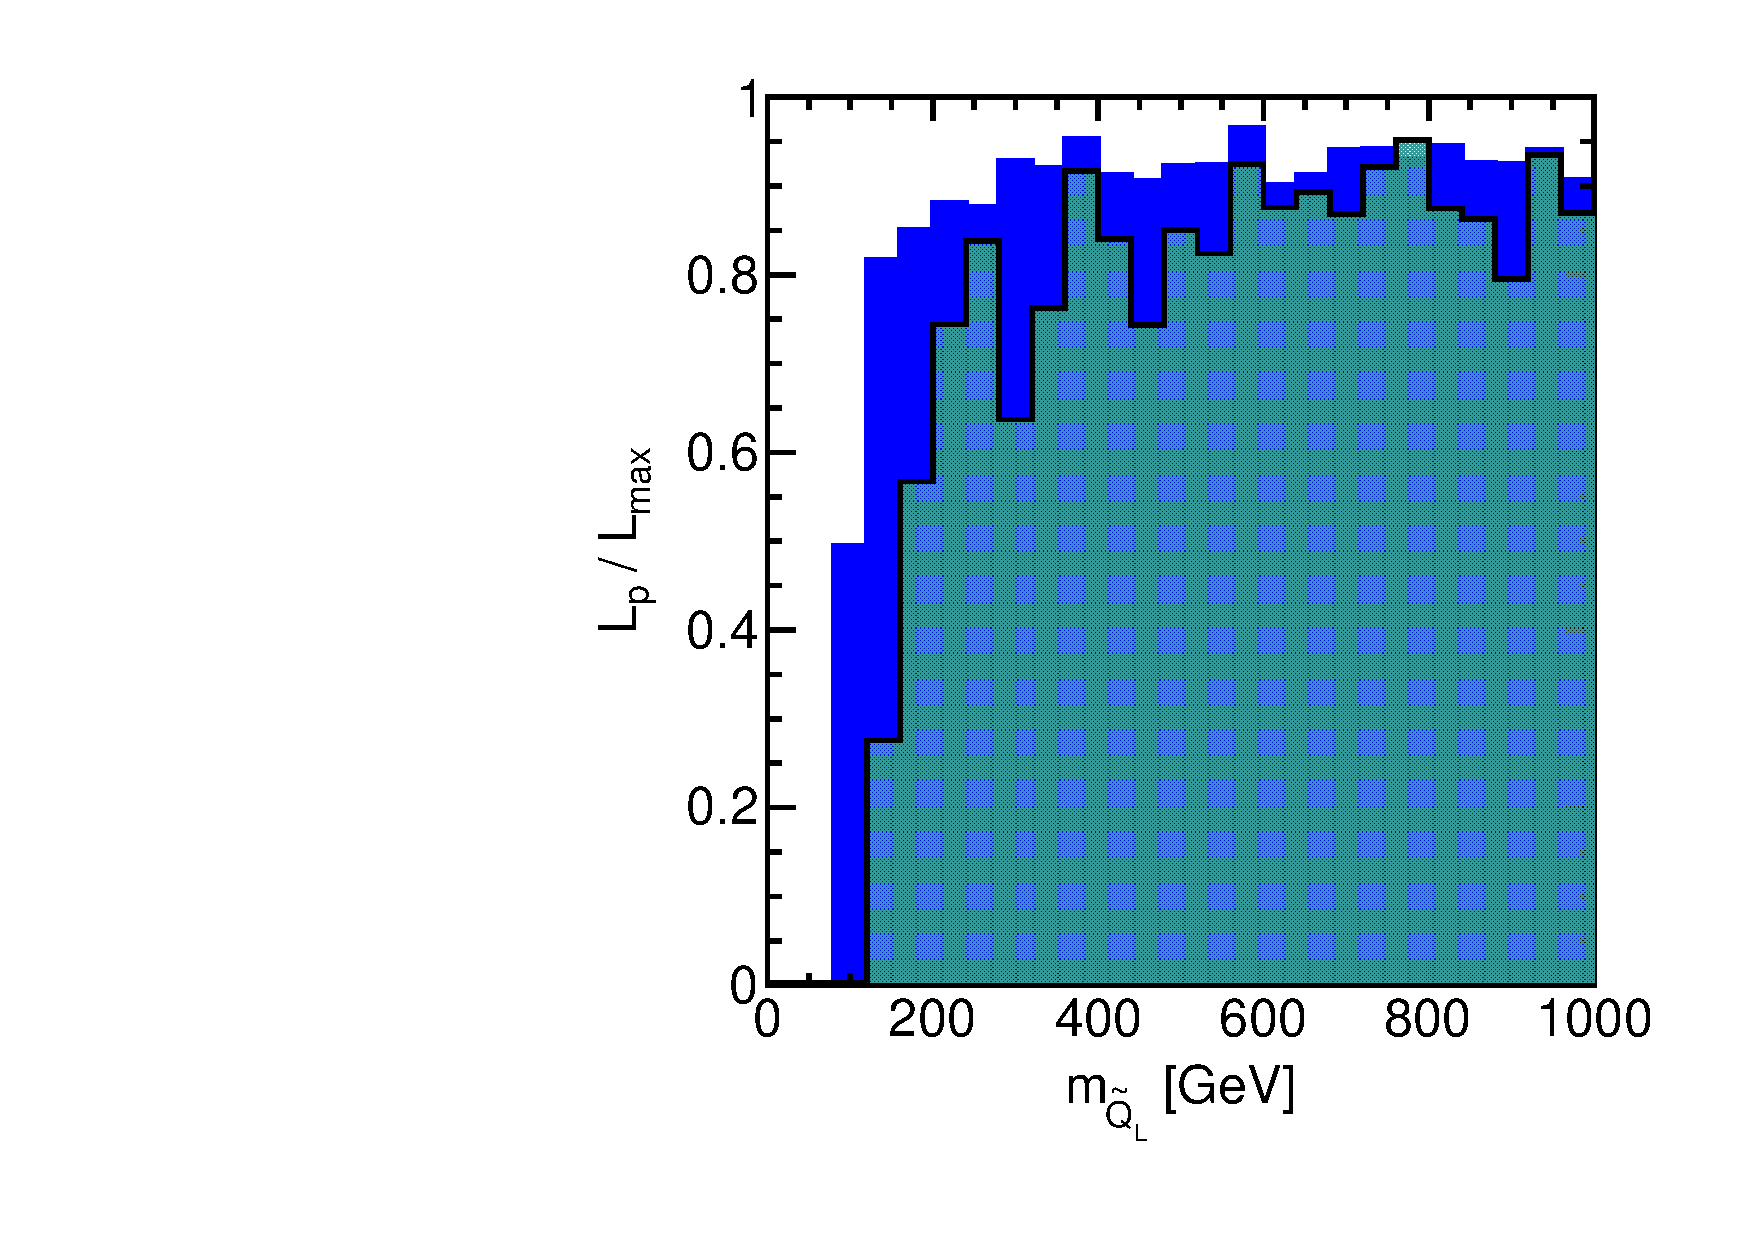
\includegraphics[height=5.5cm]{figs/fig_m_Q_L.pdf} 
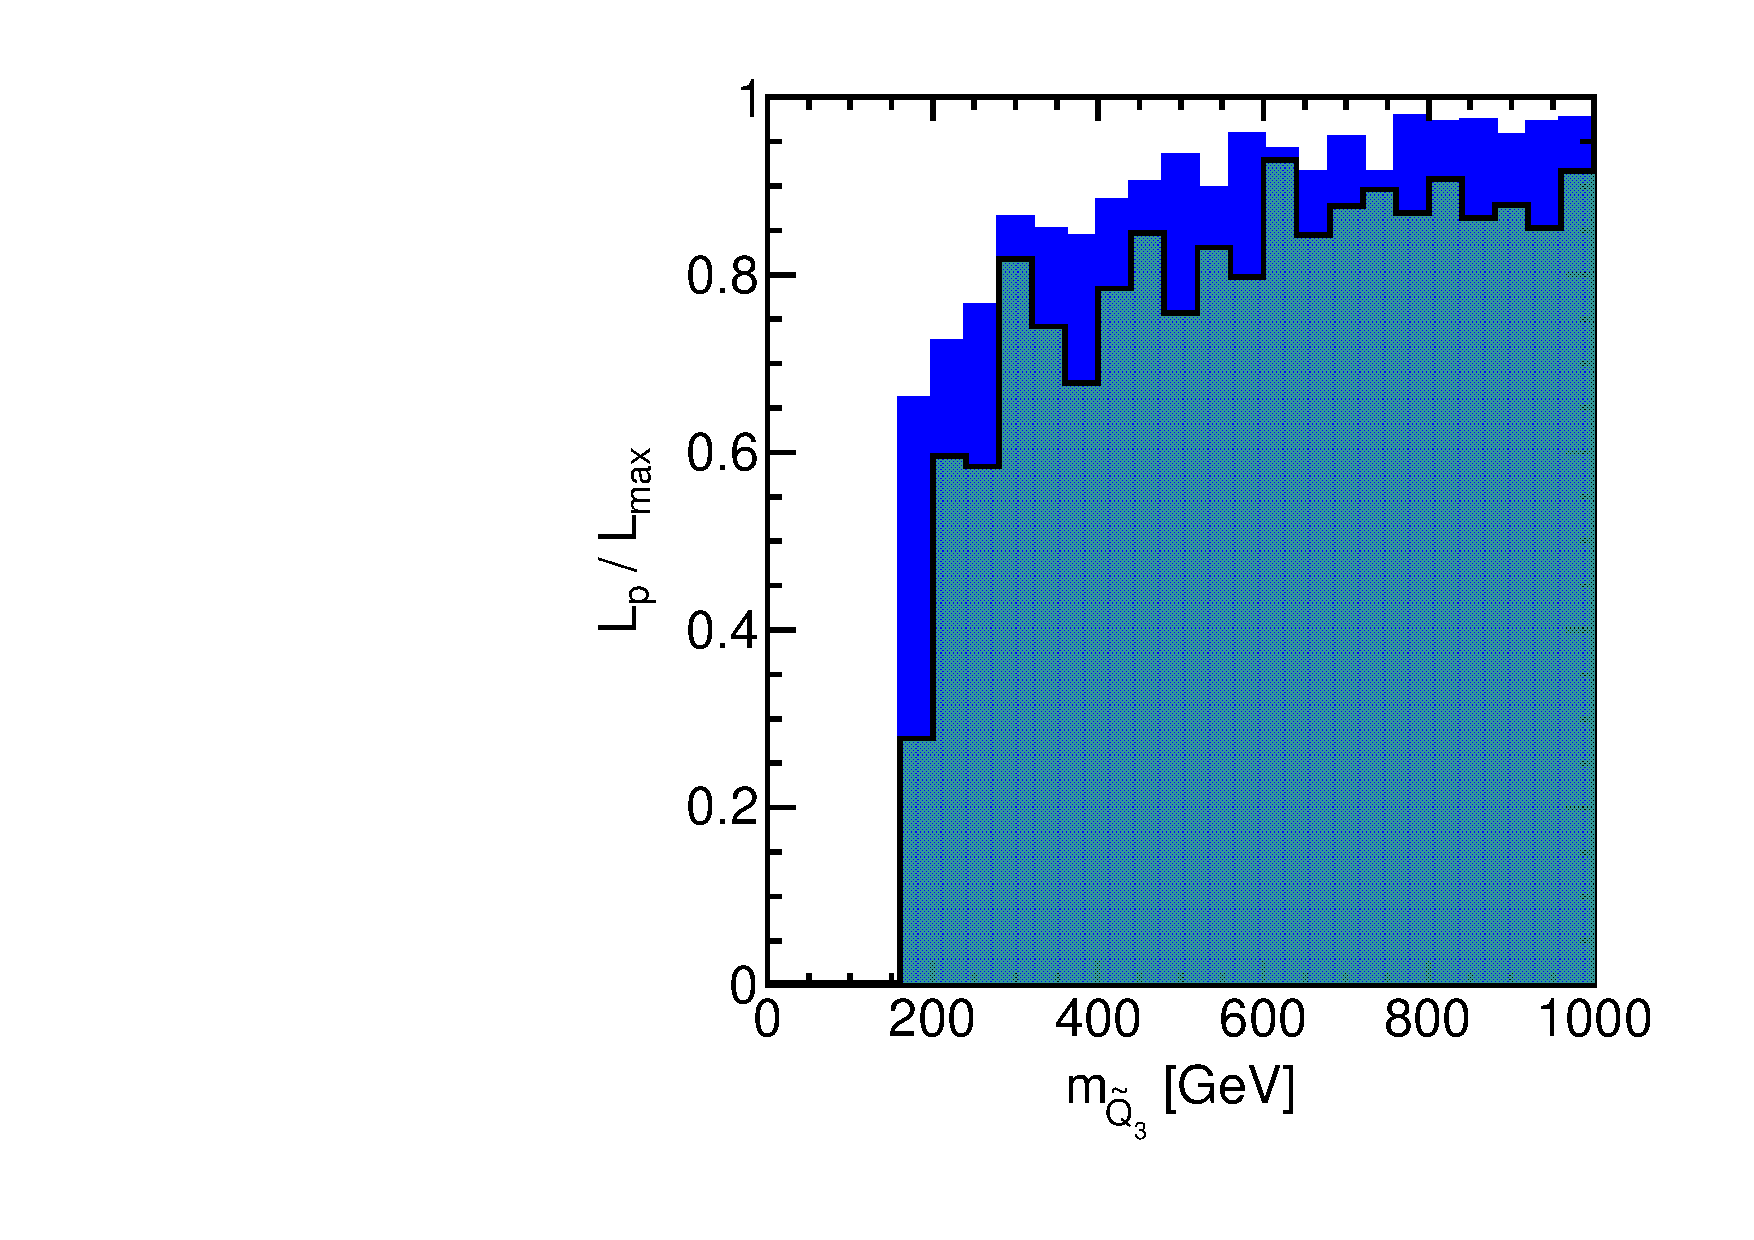
\includegraphics[height=5.5cm]{figs/fig_m_Q_3.pdf} \\
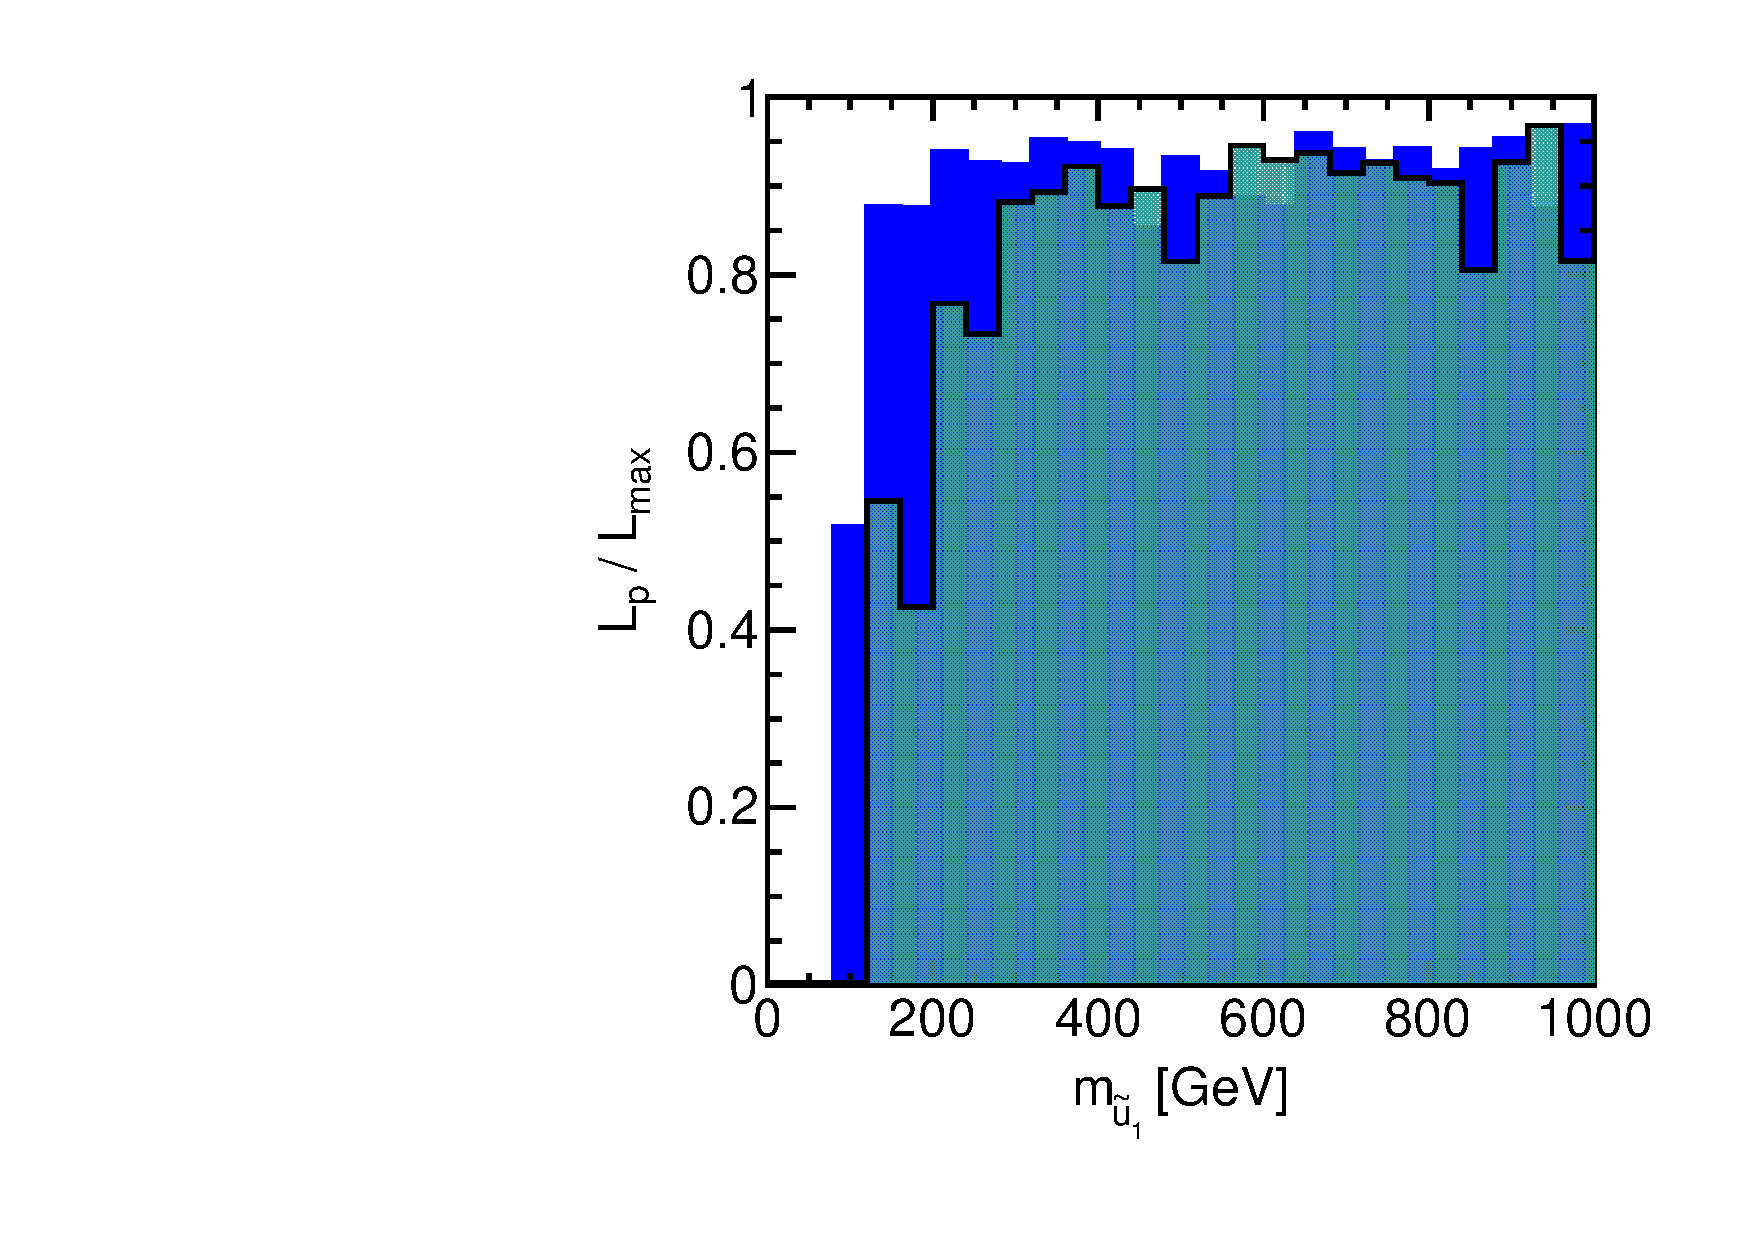
\includegraphics[height=5.5cm]{figs/fig_m_u_1.pdf}
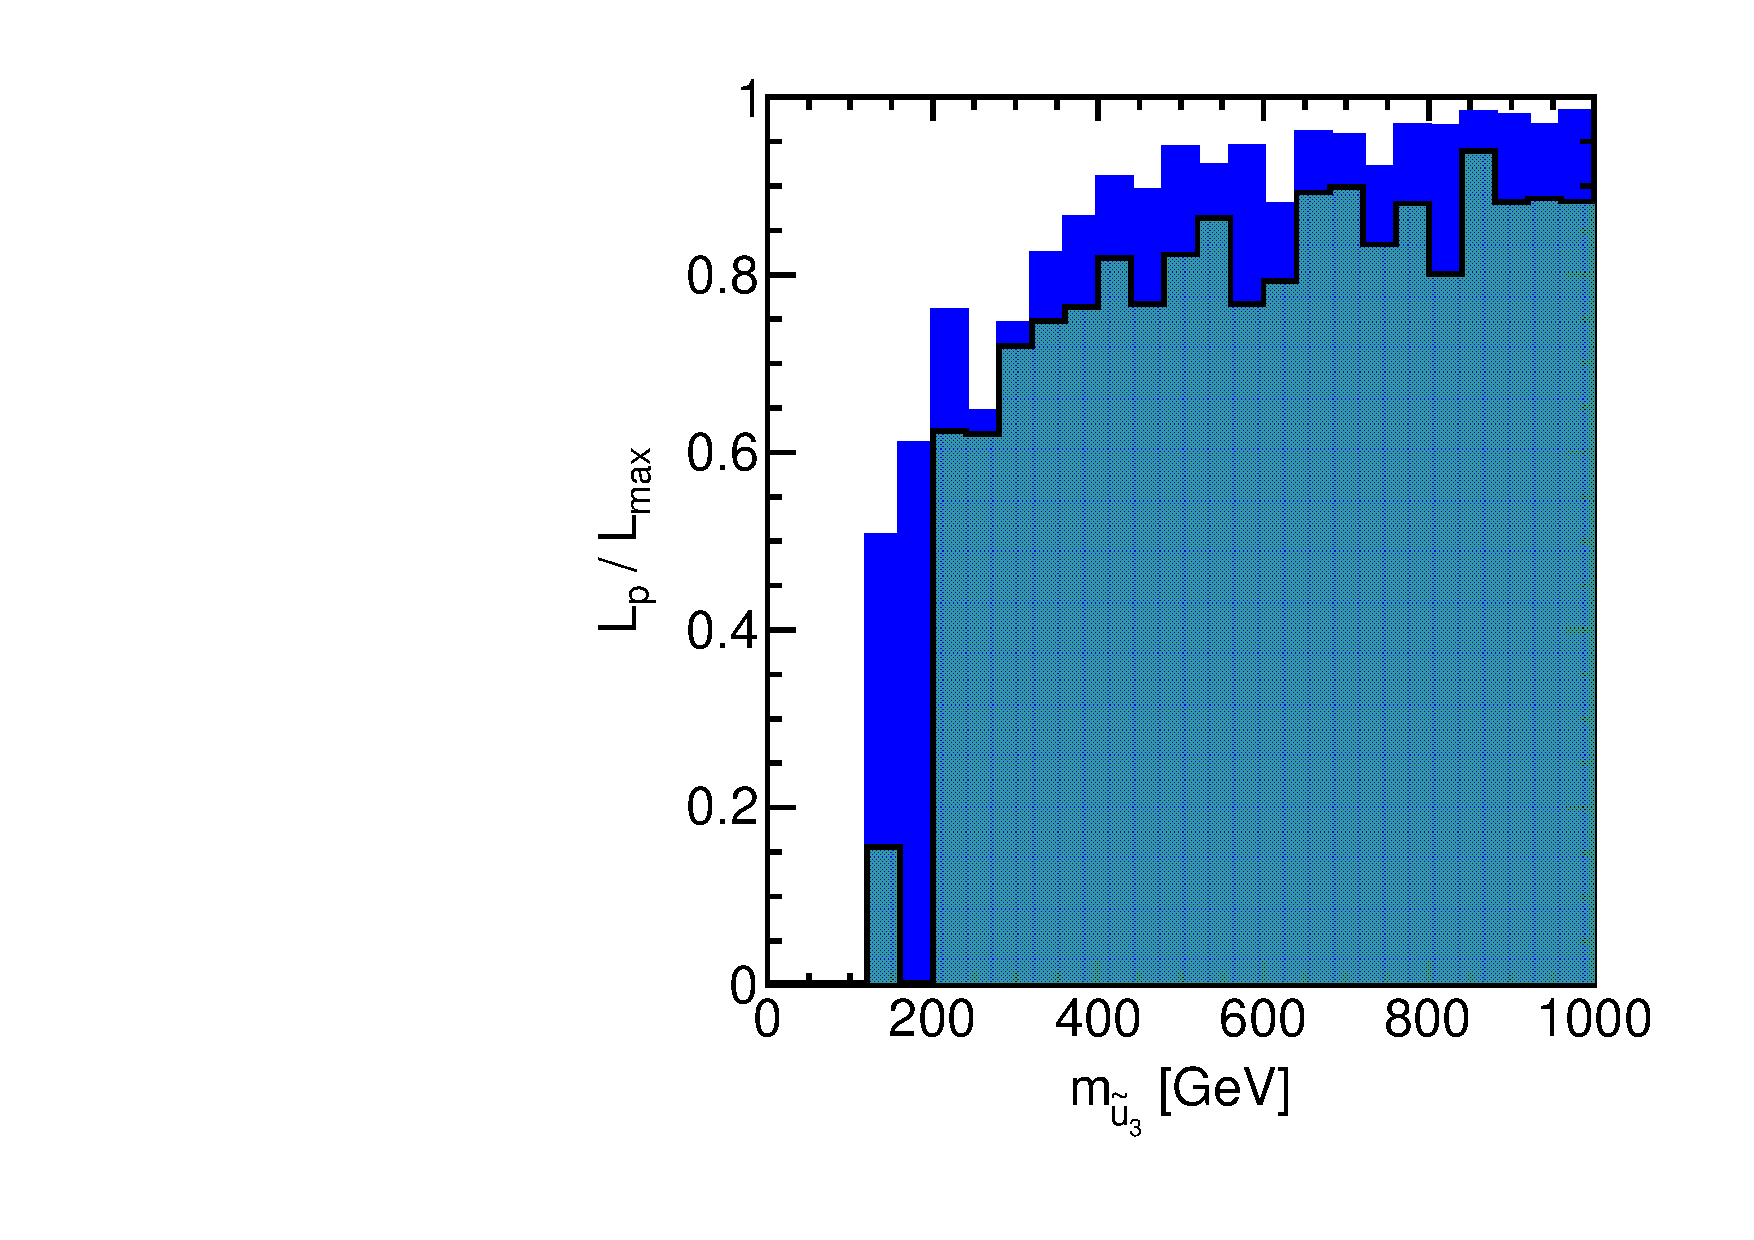
\includegraphics[height=5.5cm]{figs/fig_m_u_3.pdf} \\
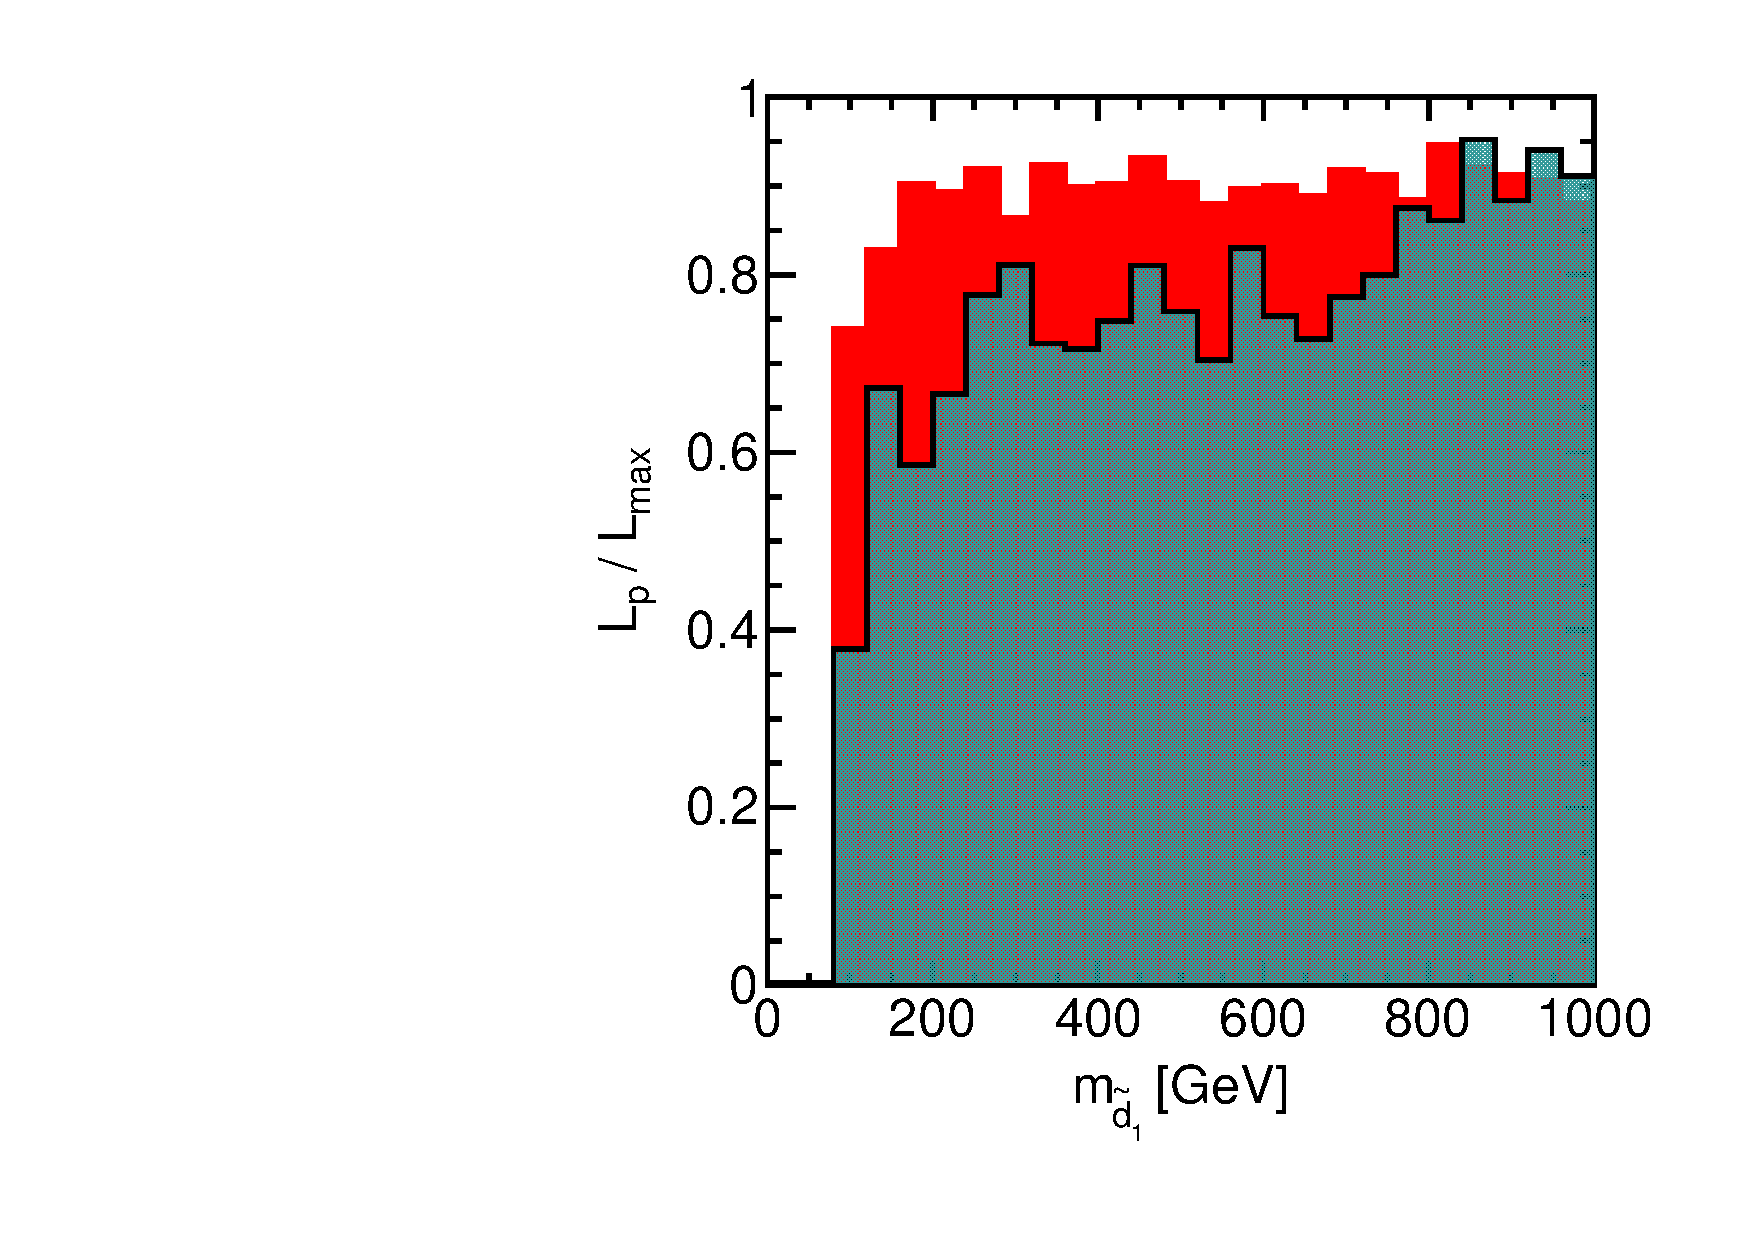
\includegraphics[height=5.5cm]{figs/fig_m_d_1.pdf}
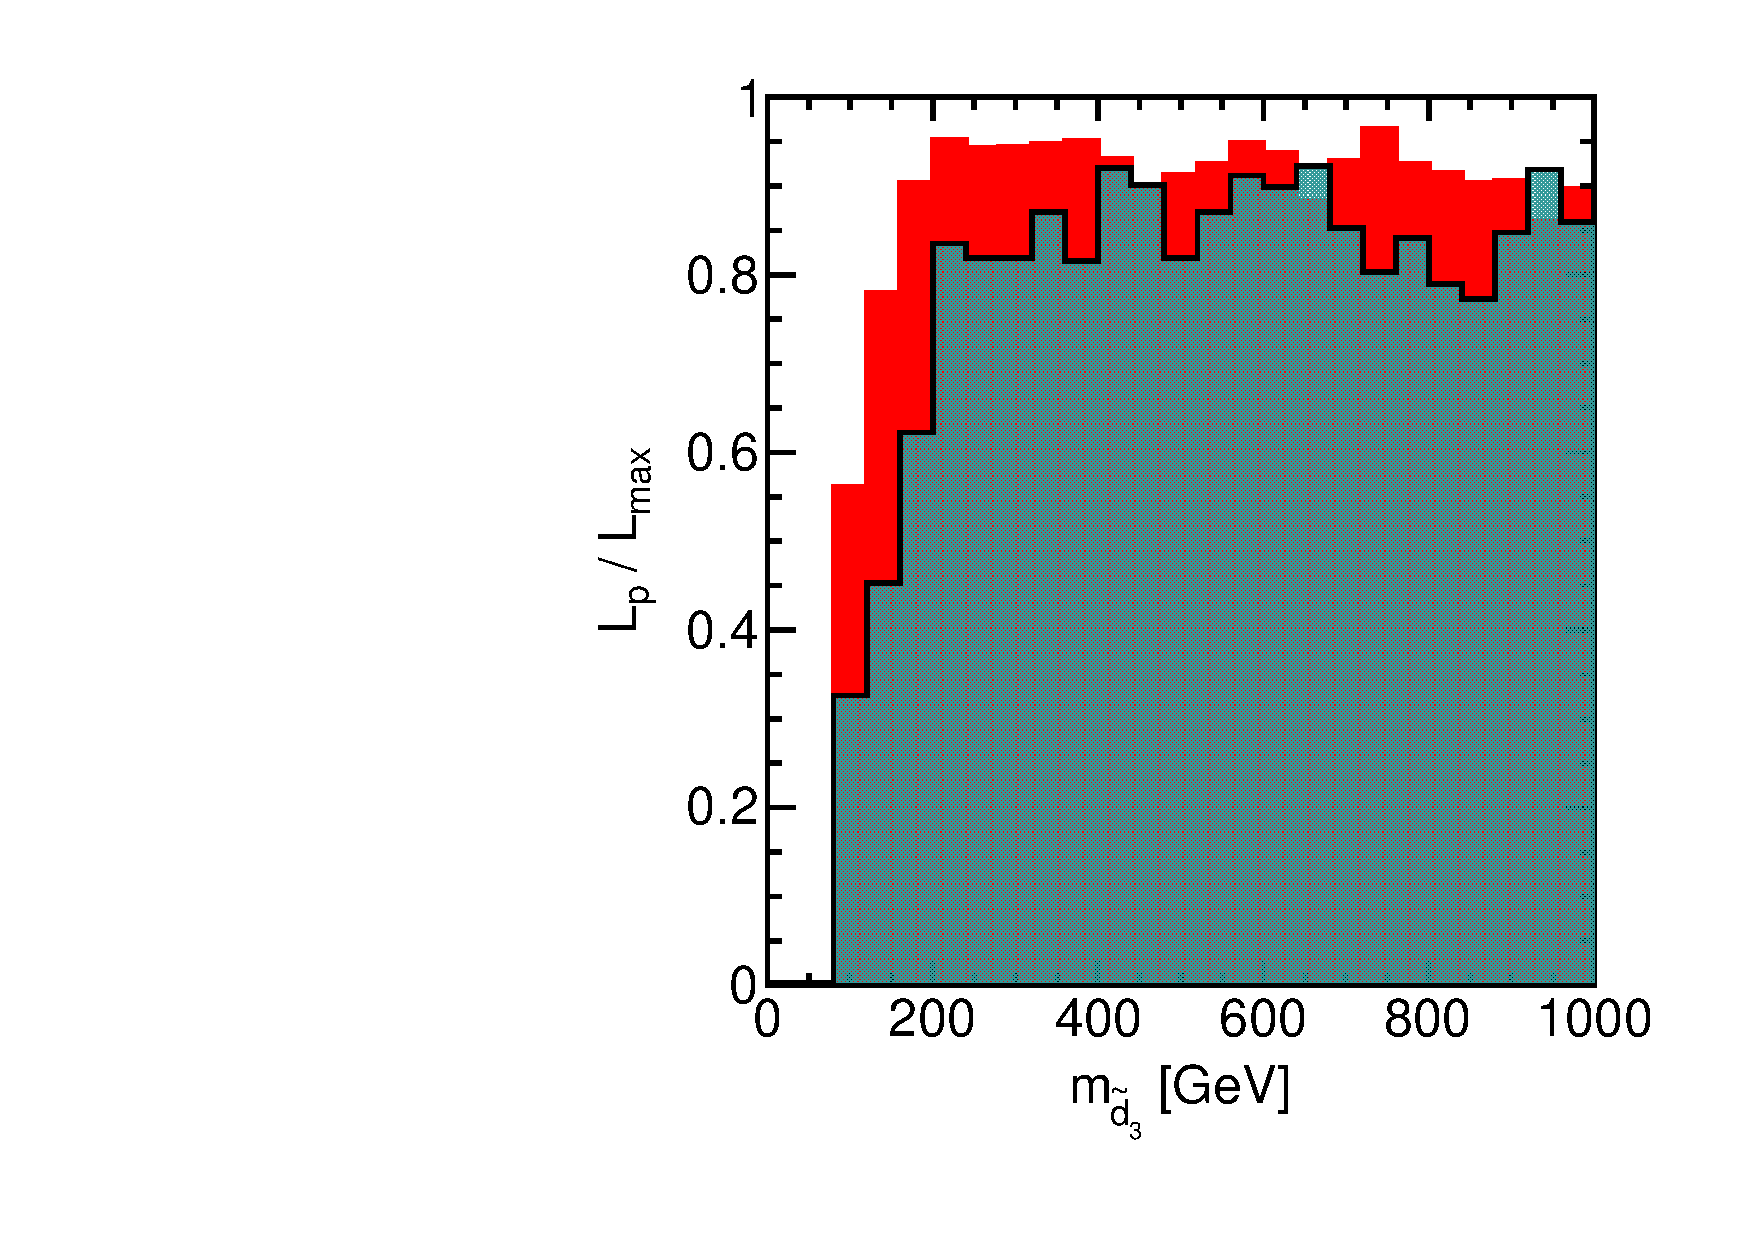
\includegraphics[height=5.5cm]{figs/fig_m_d_3.pdf}
\caption{Ratios of profile likelihood $L_p$ to maximum likelihood $L_{max}$ shown for the squark mass parameters at SUSY scale.  The colored and shaded histograms show the distributions before and after the inclusion of the CMS results.}
\label{fig:LRwcms_msq}
\end{center}
\end{figure}


\begin{figure}[htbp]
\begin{center}
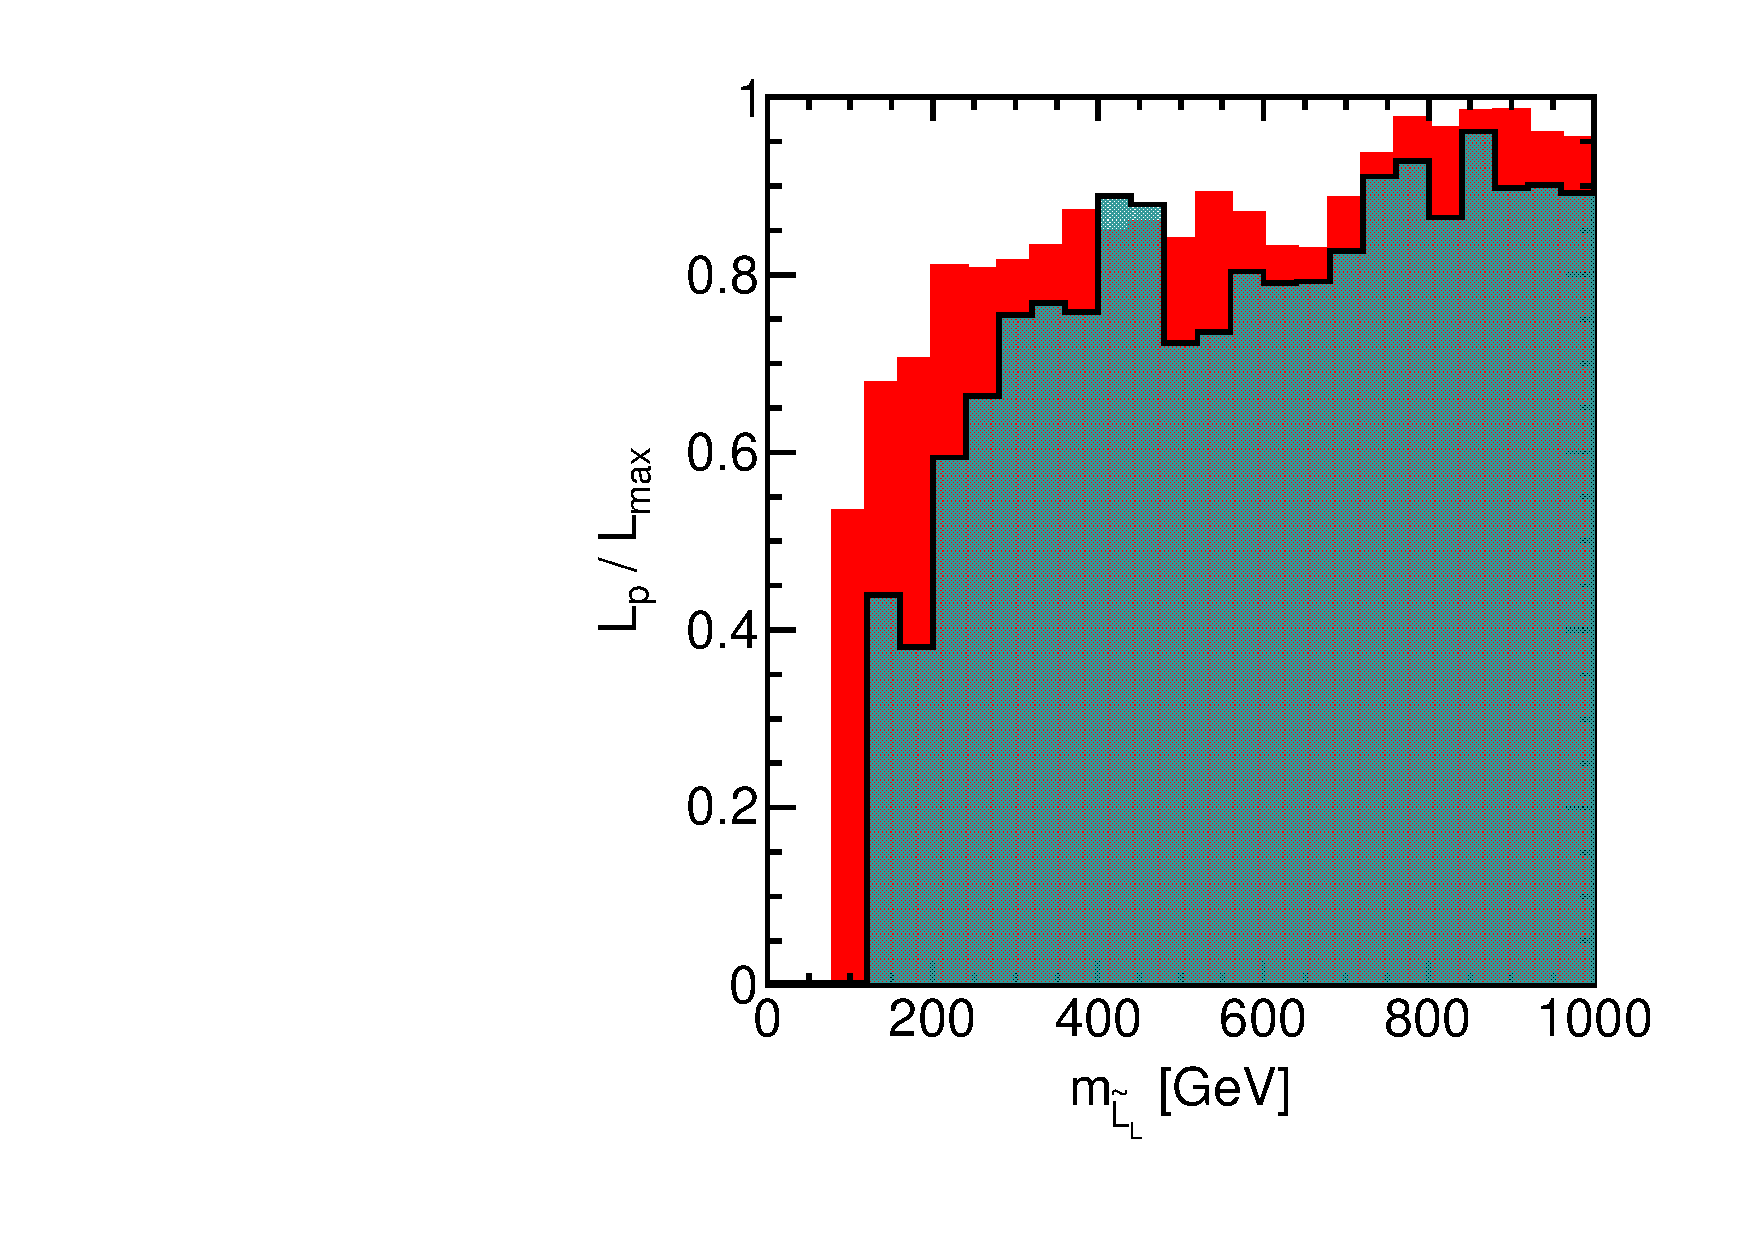
\includegraphics[height=5.5cm]{figs/fig_m_L_L.pdf} 
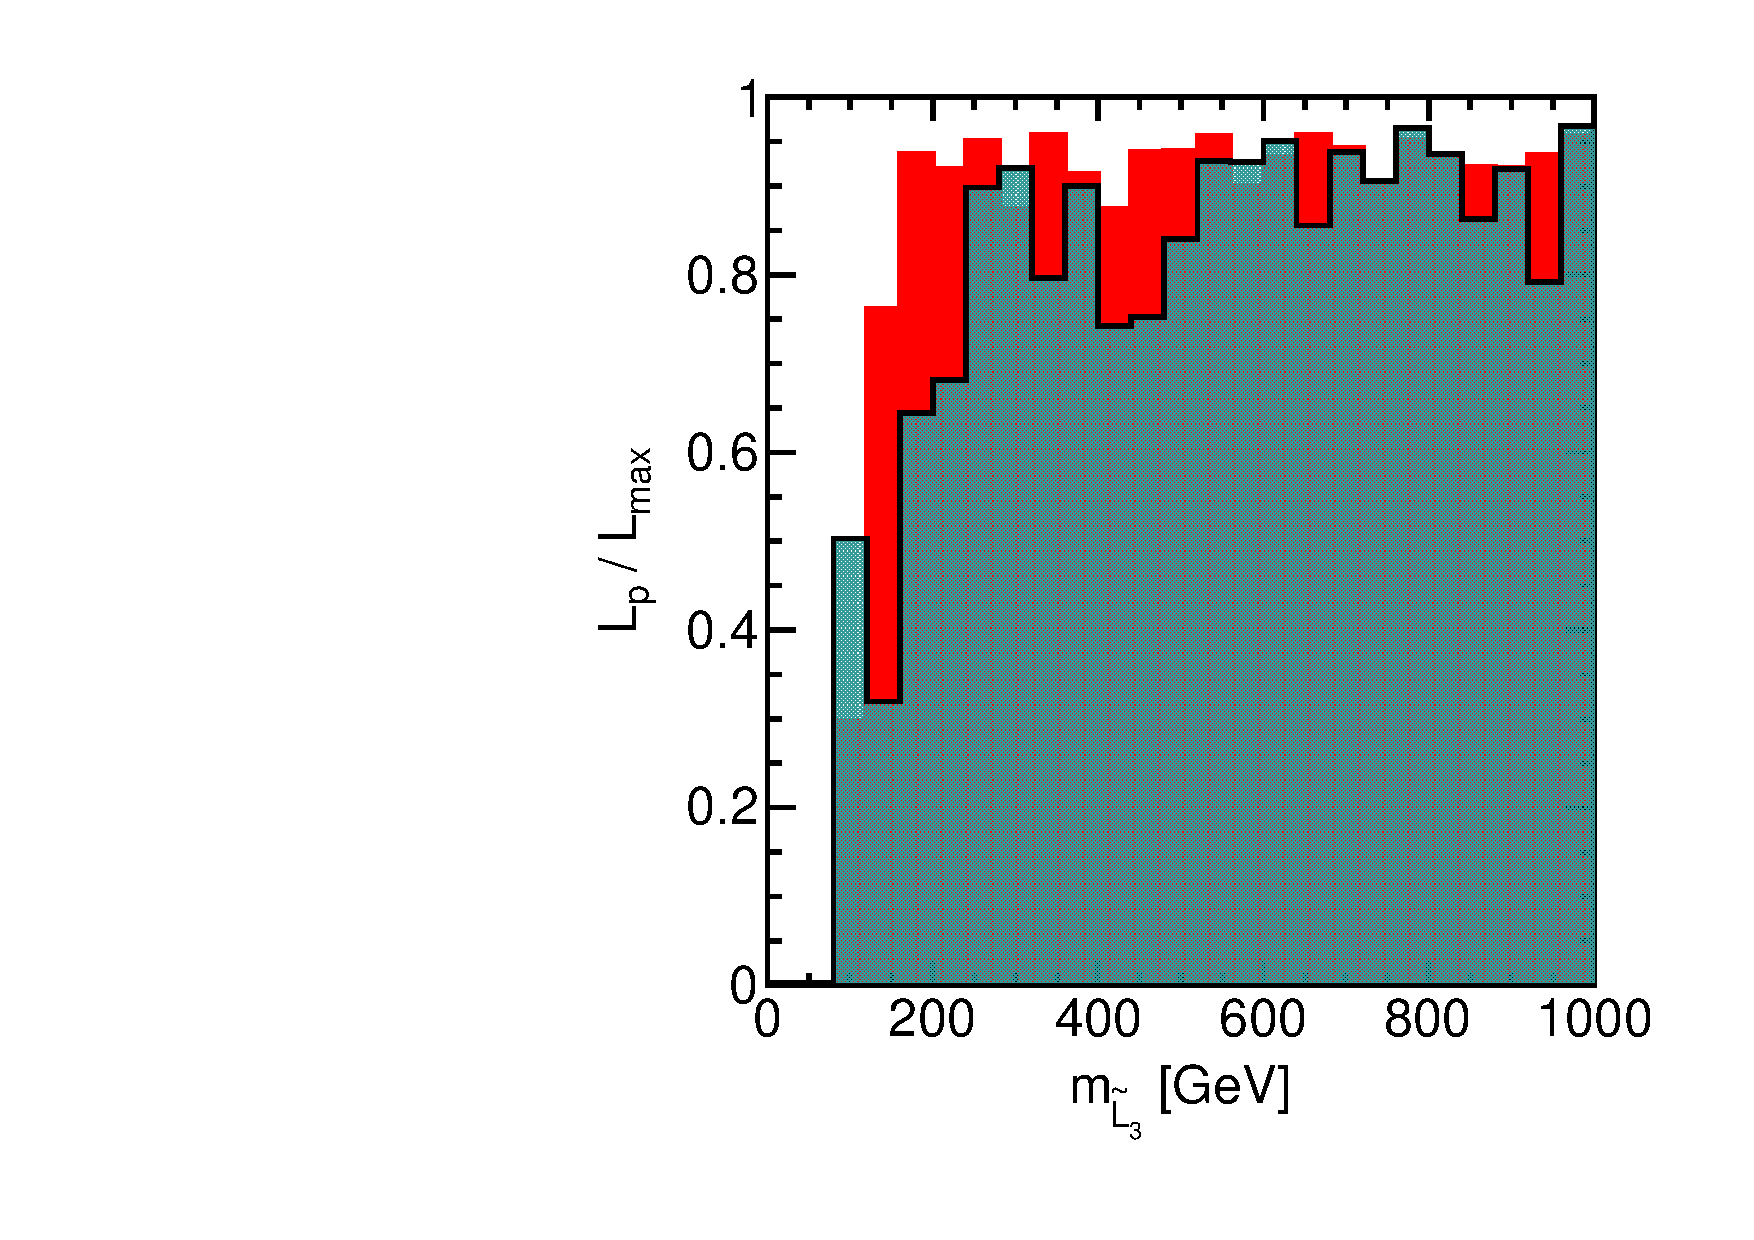
\includegraphics[height=5.5cm]{figs/fig_m_L_3.pdf} \\
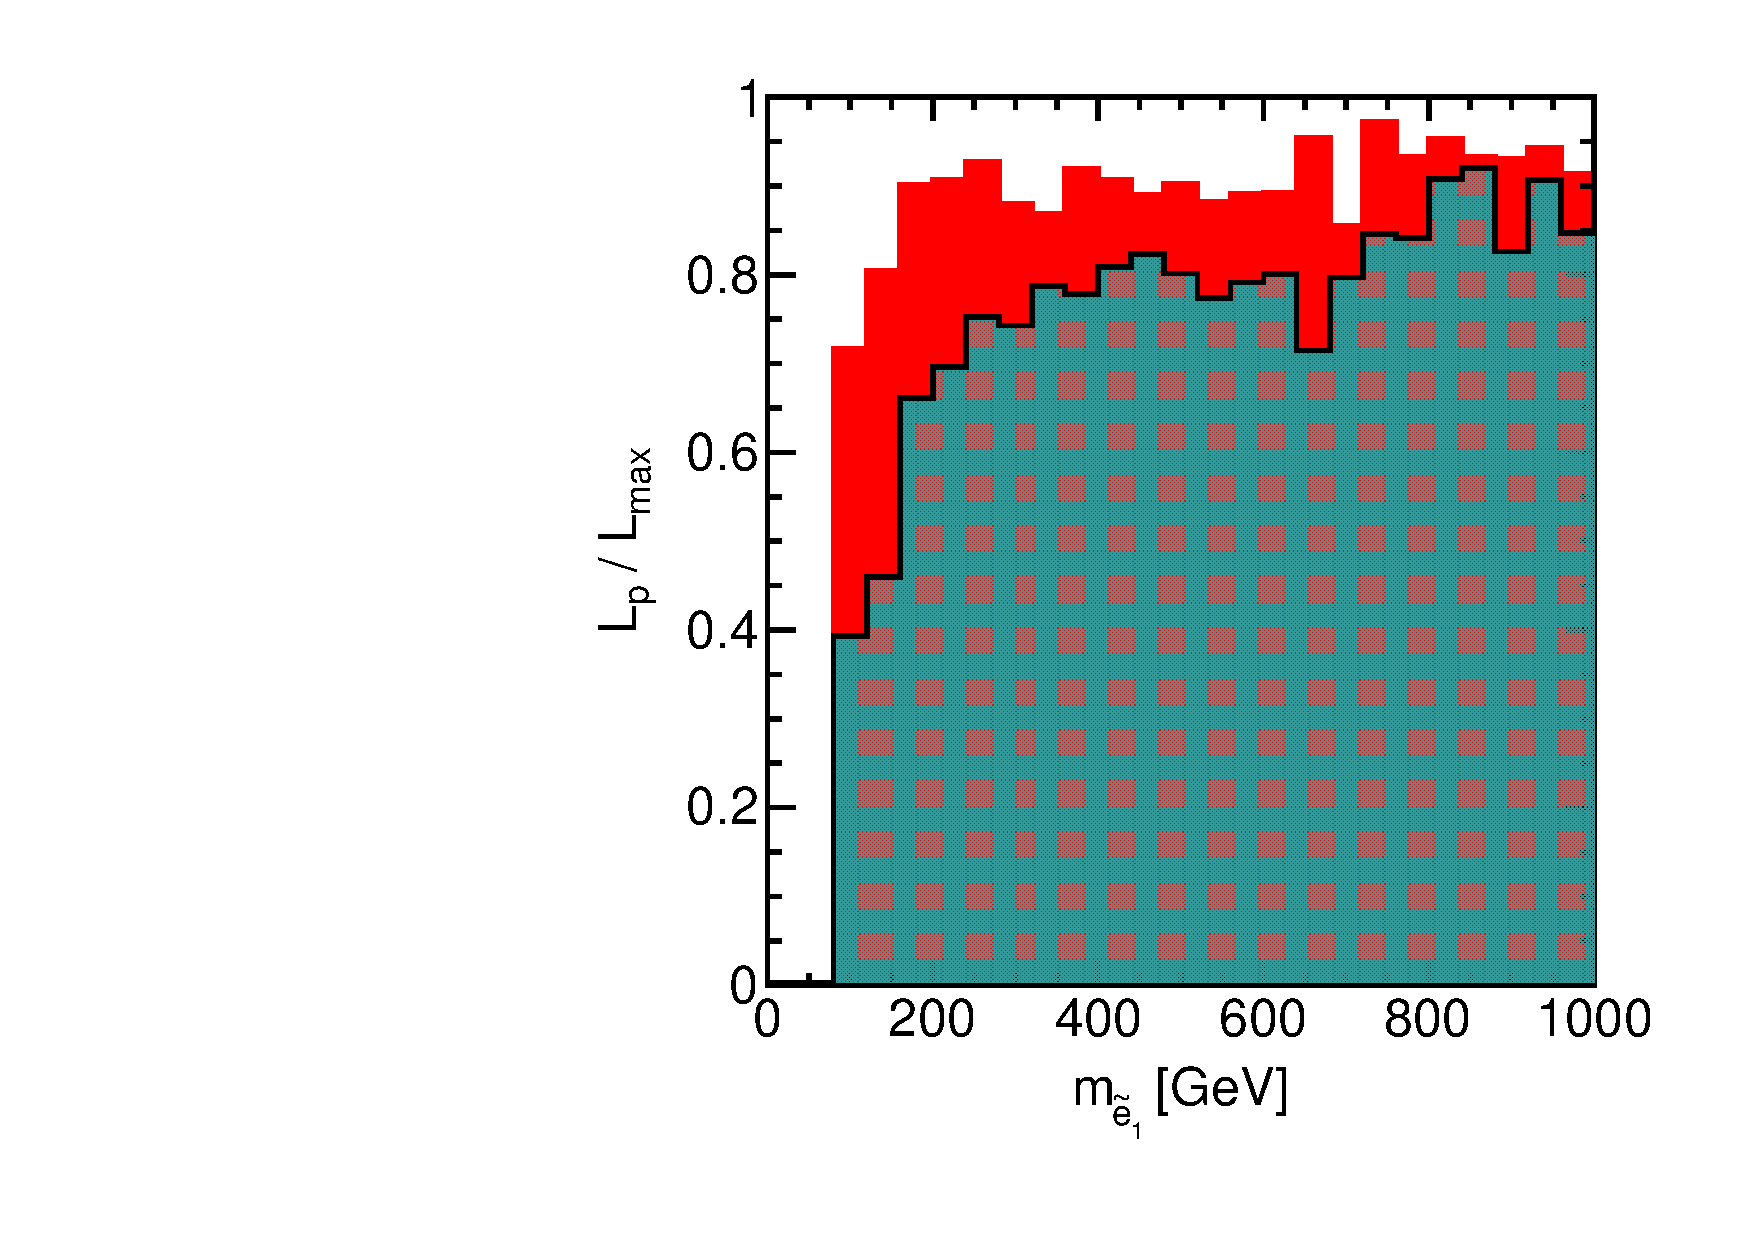
\includegraphics[height=5.5cm]{figs/fig_m_e_1.pdf}
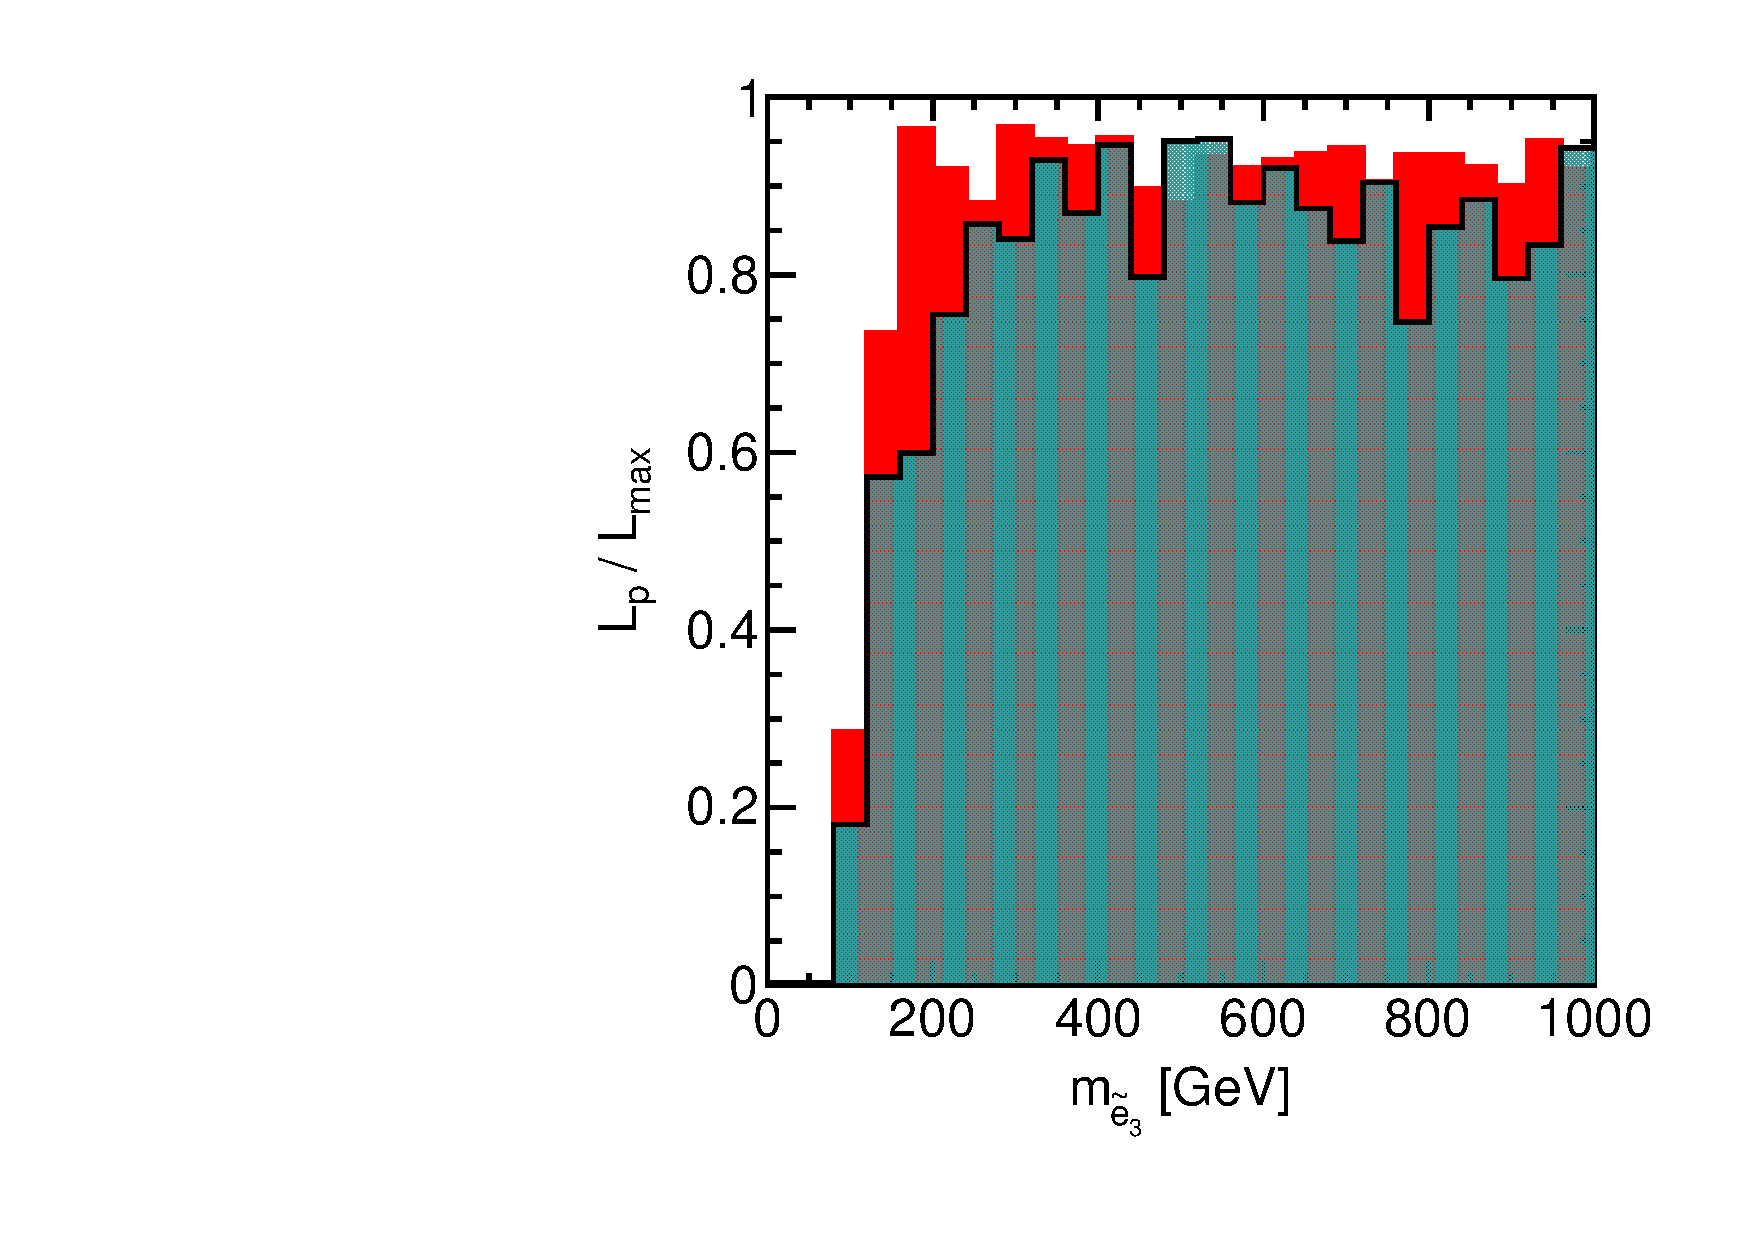
\includegraphics[height=5.5cm]{figs/fig_m_e_3.pdf}
\caption{Ratios of profile likelihood $L_p$ to maximum likelihood $L_{max}$ shown for the slepton mass parameters at SUSY scale.  The colored and shaded histograms show the distributions before and after the inclusion of the CMS results.}
\label{fig:LRwcms_msl}
\end{center}
\end{figure}


\begin{figure}[htbp]
\begin{center}
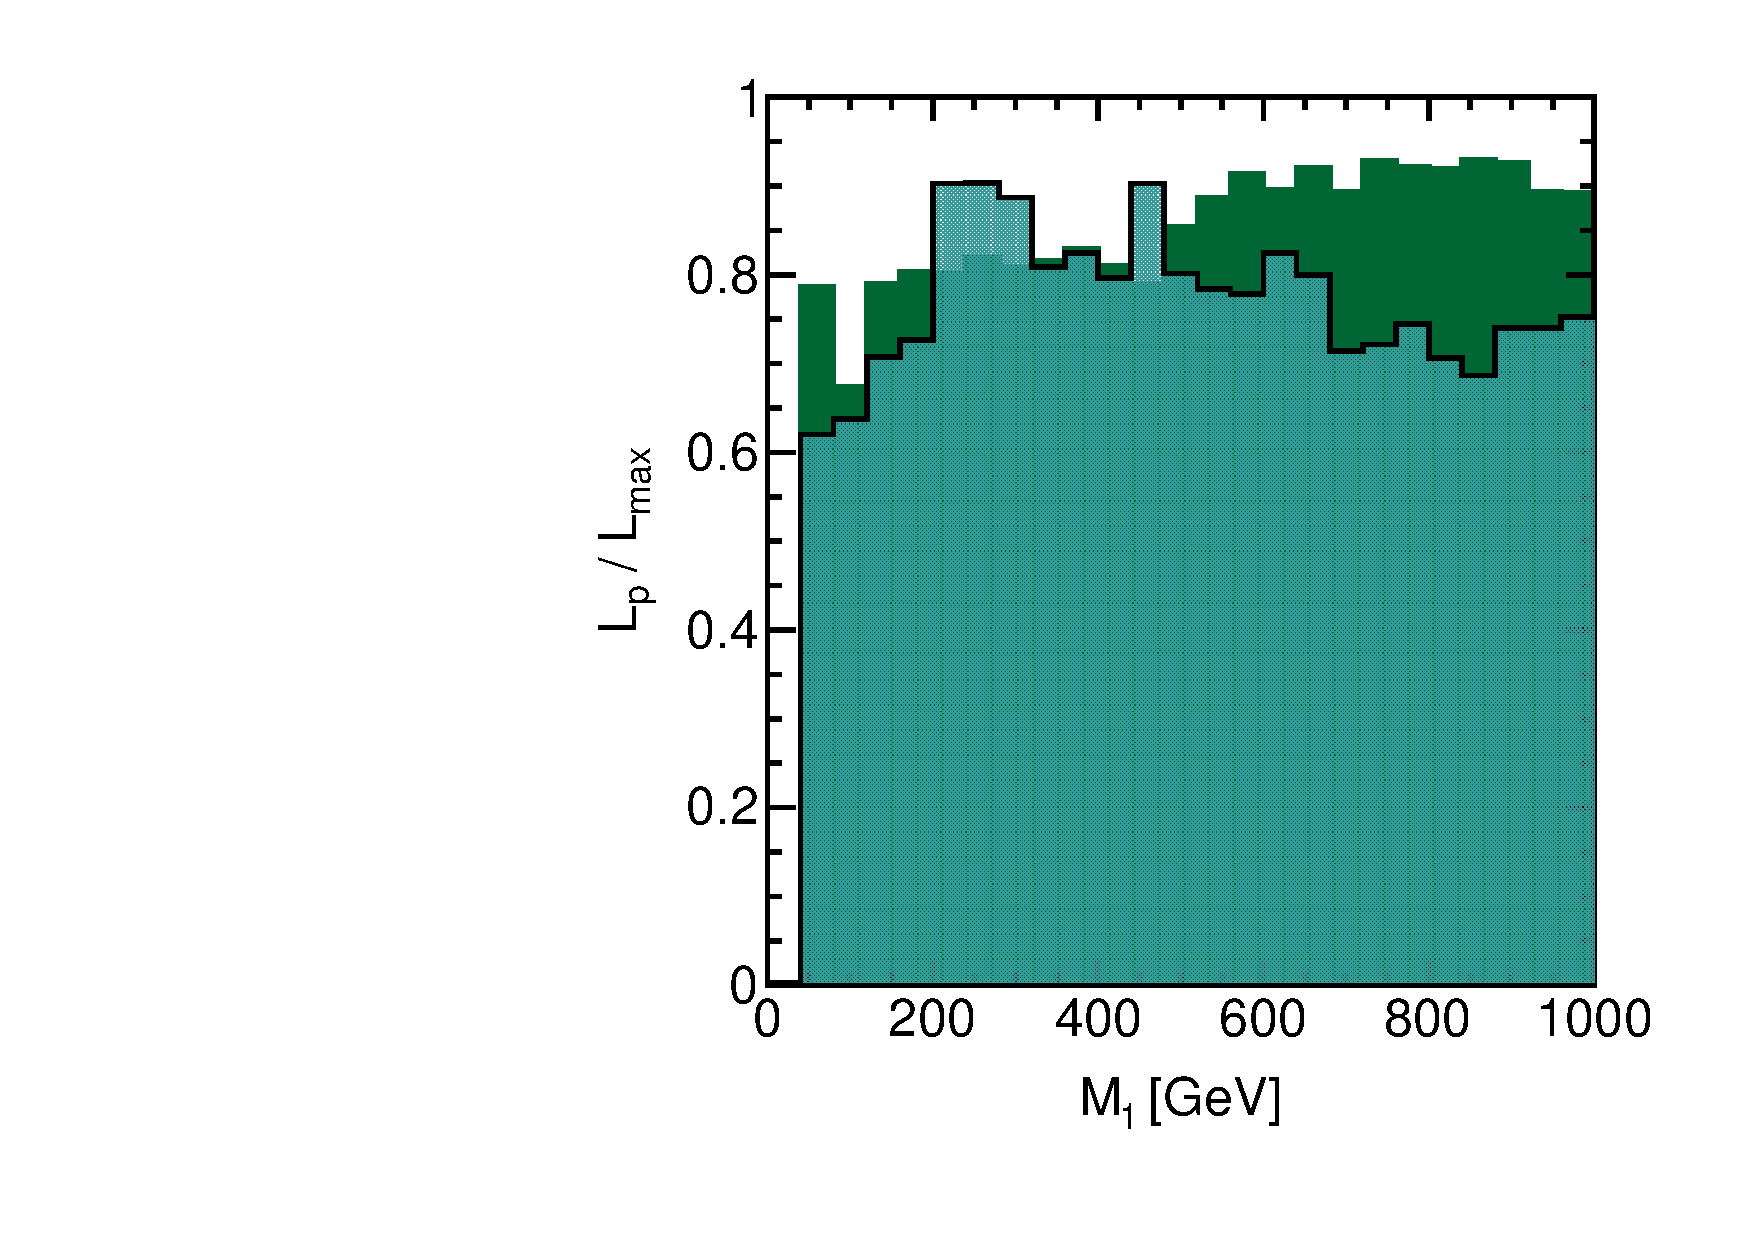
\includegraphics[height=5.5cm]{figs/fig_M_1.pdf} 
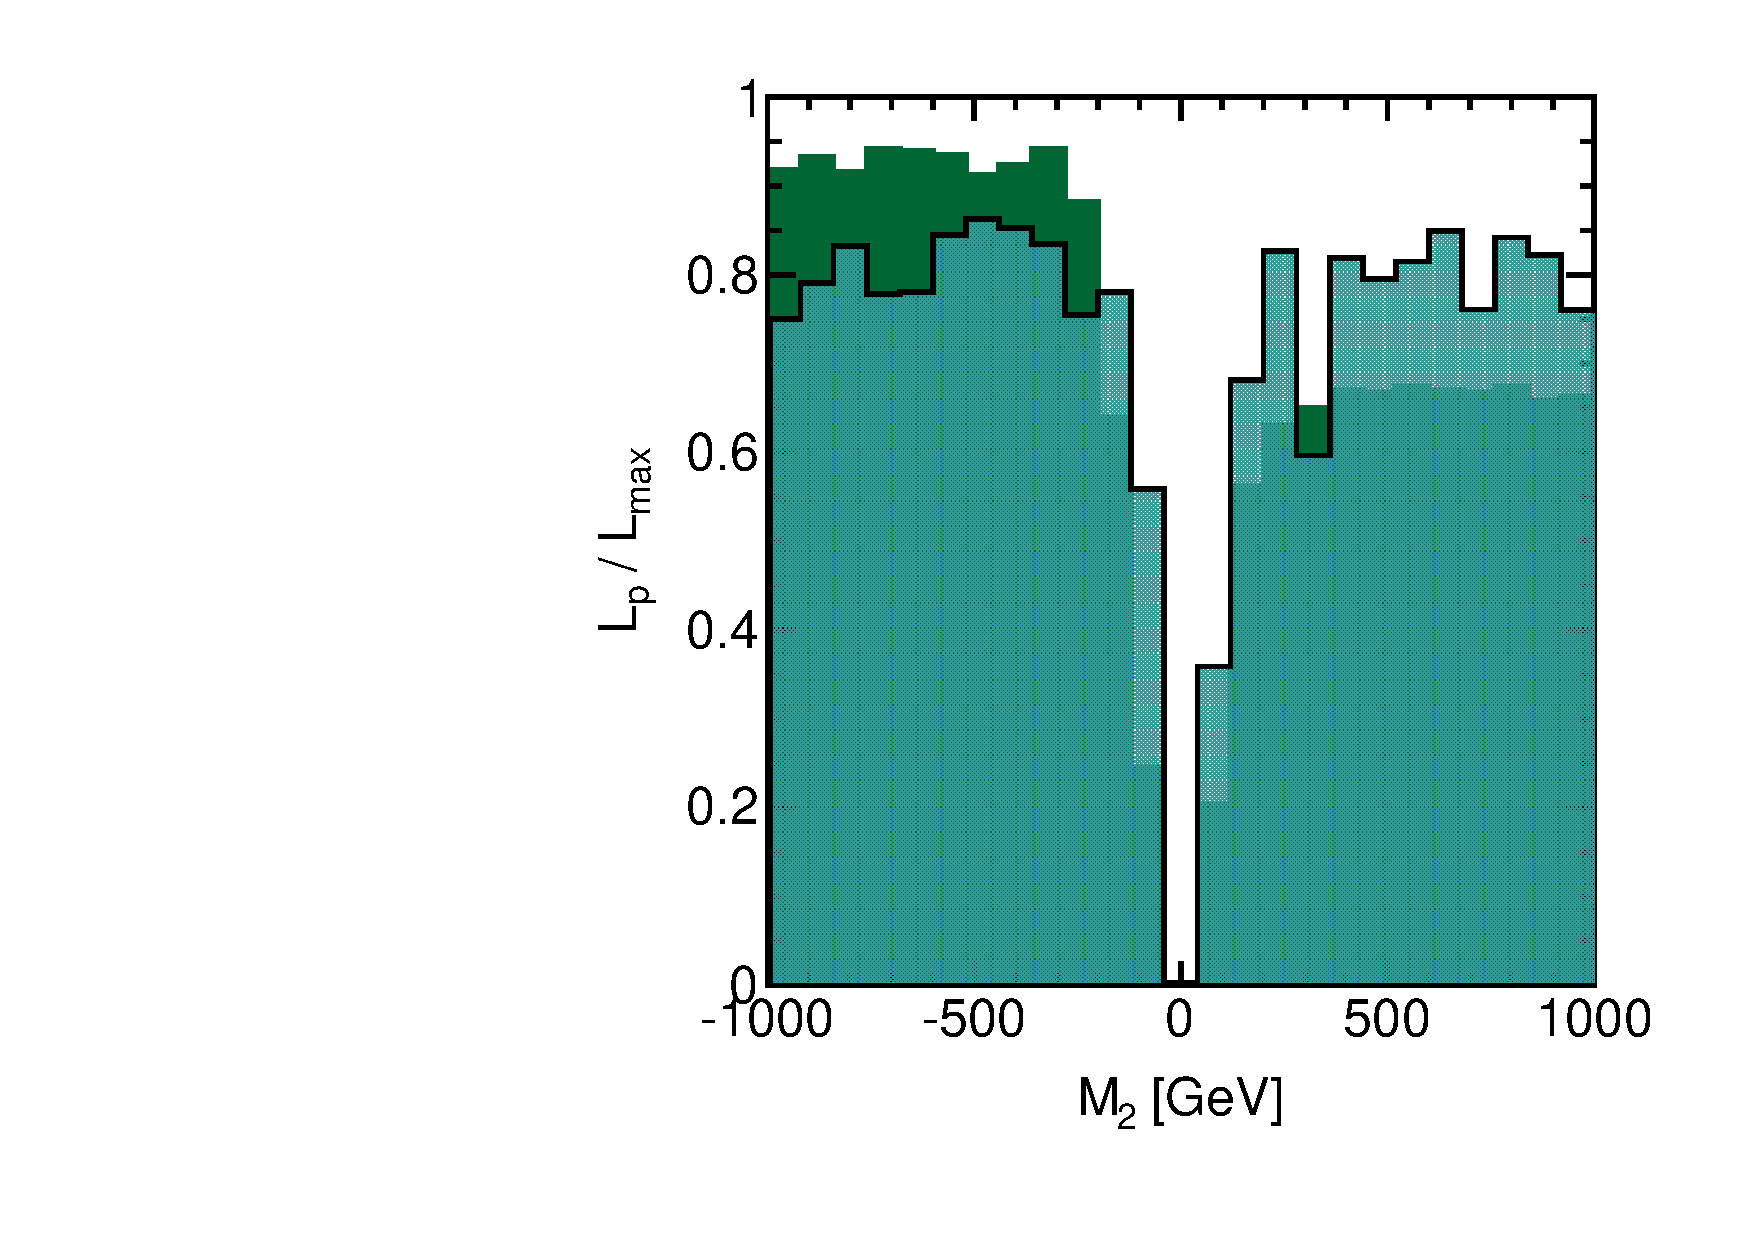
\includegraphics[height=5.5cm]{figs/fig_M_2.pdf} \\
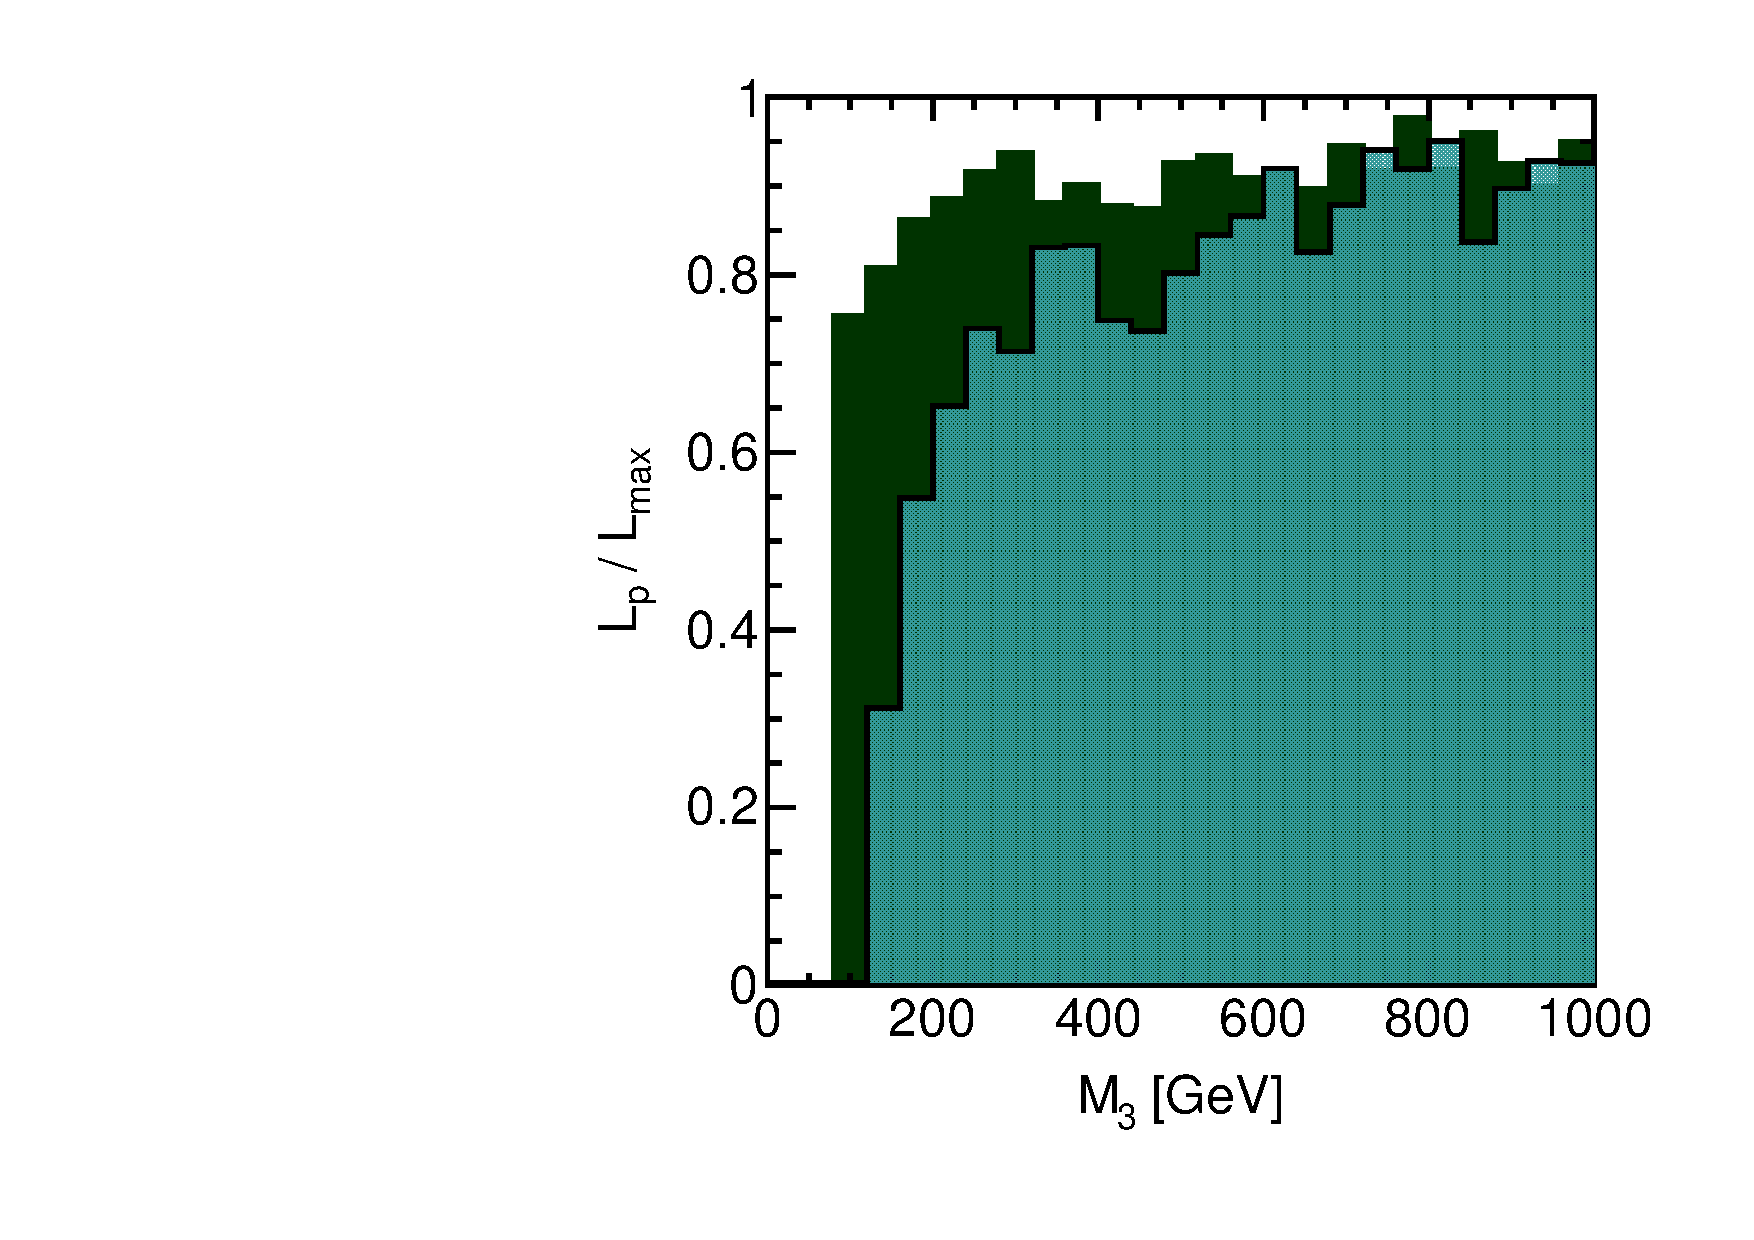
\includegraphics[height=5.5cm]{figs/fig_M_3.pdf}
\caption{Ratios of profile likelihood $L_p$ to maximum likelihood $L_{max}$ shown for gaugino mass parameters at  SUSY scale.  The colored and shaded histograms show the distributions before and after the inclusion of the CMS results.}
\label{fig:LRwcms_M}
\end{center}
\end{figure}


\begin{figure}[htbp]
\begin{center}
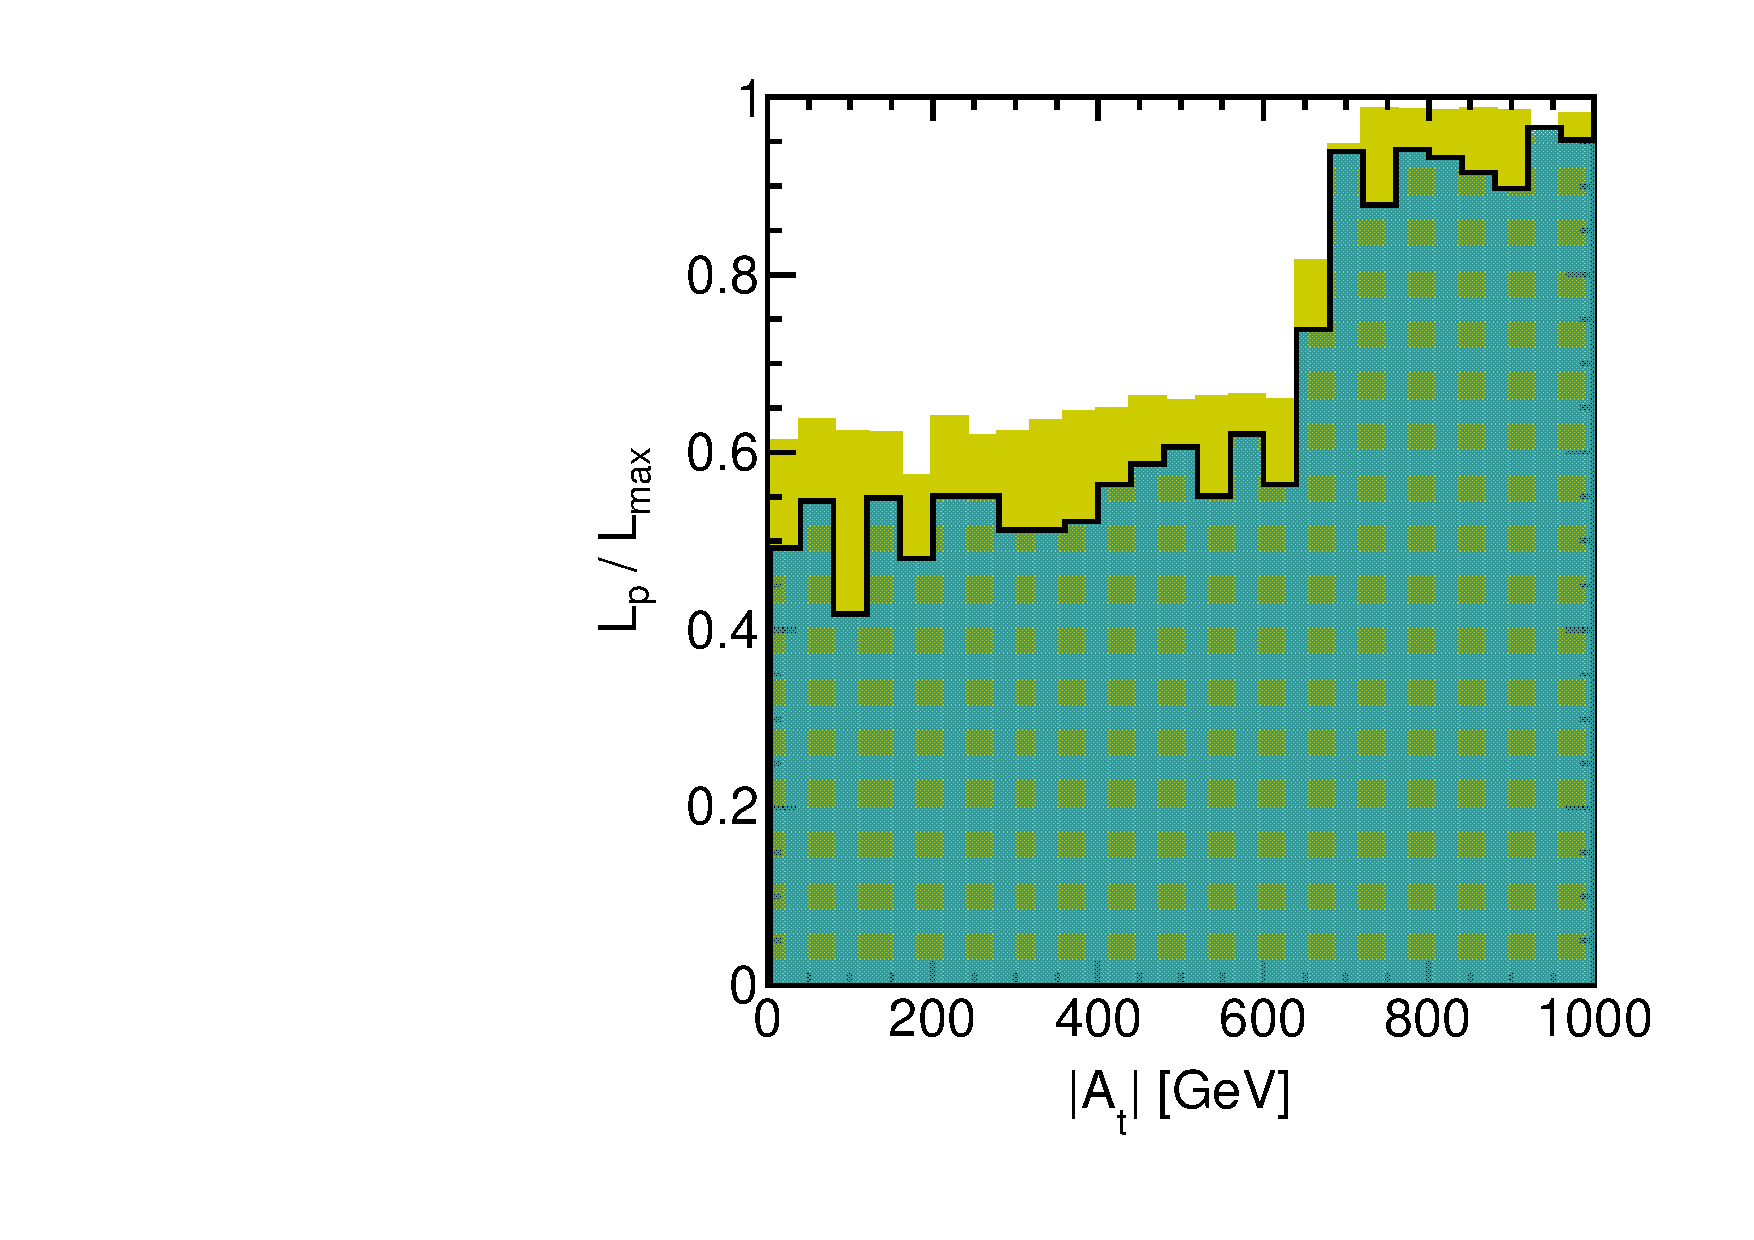
\includegraphics[height=5.5cm]{figs/fig_A_t.pdf} 
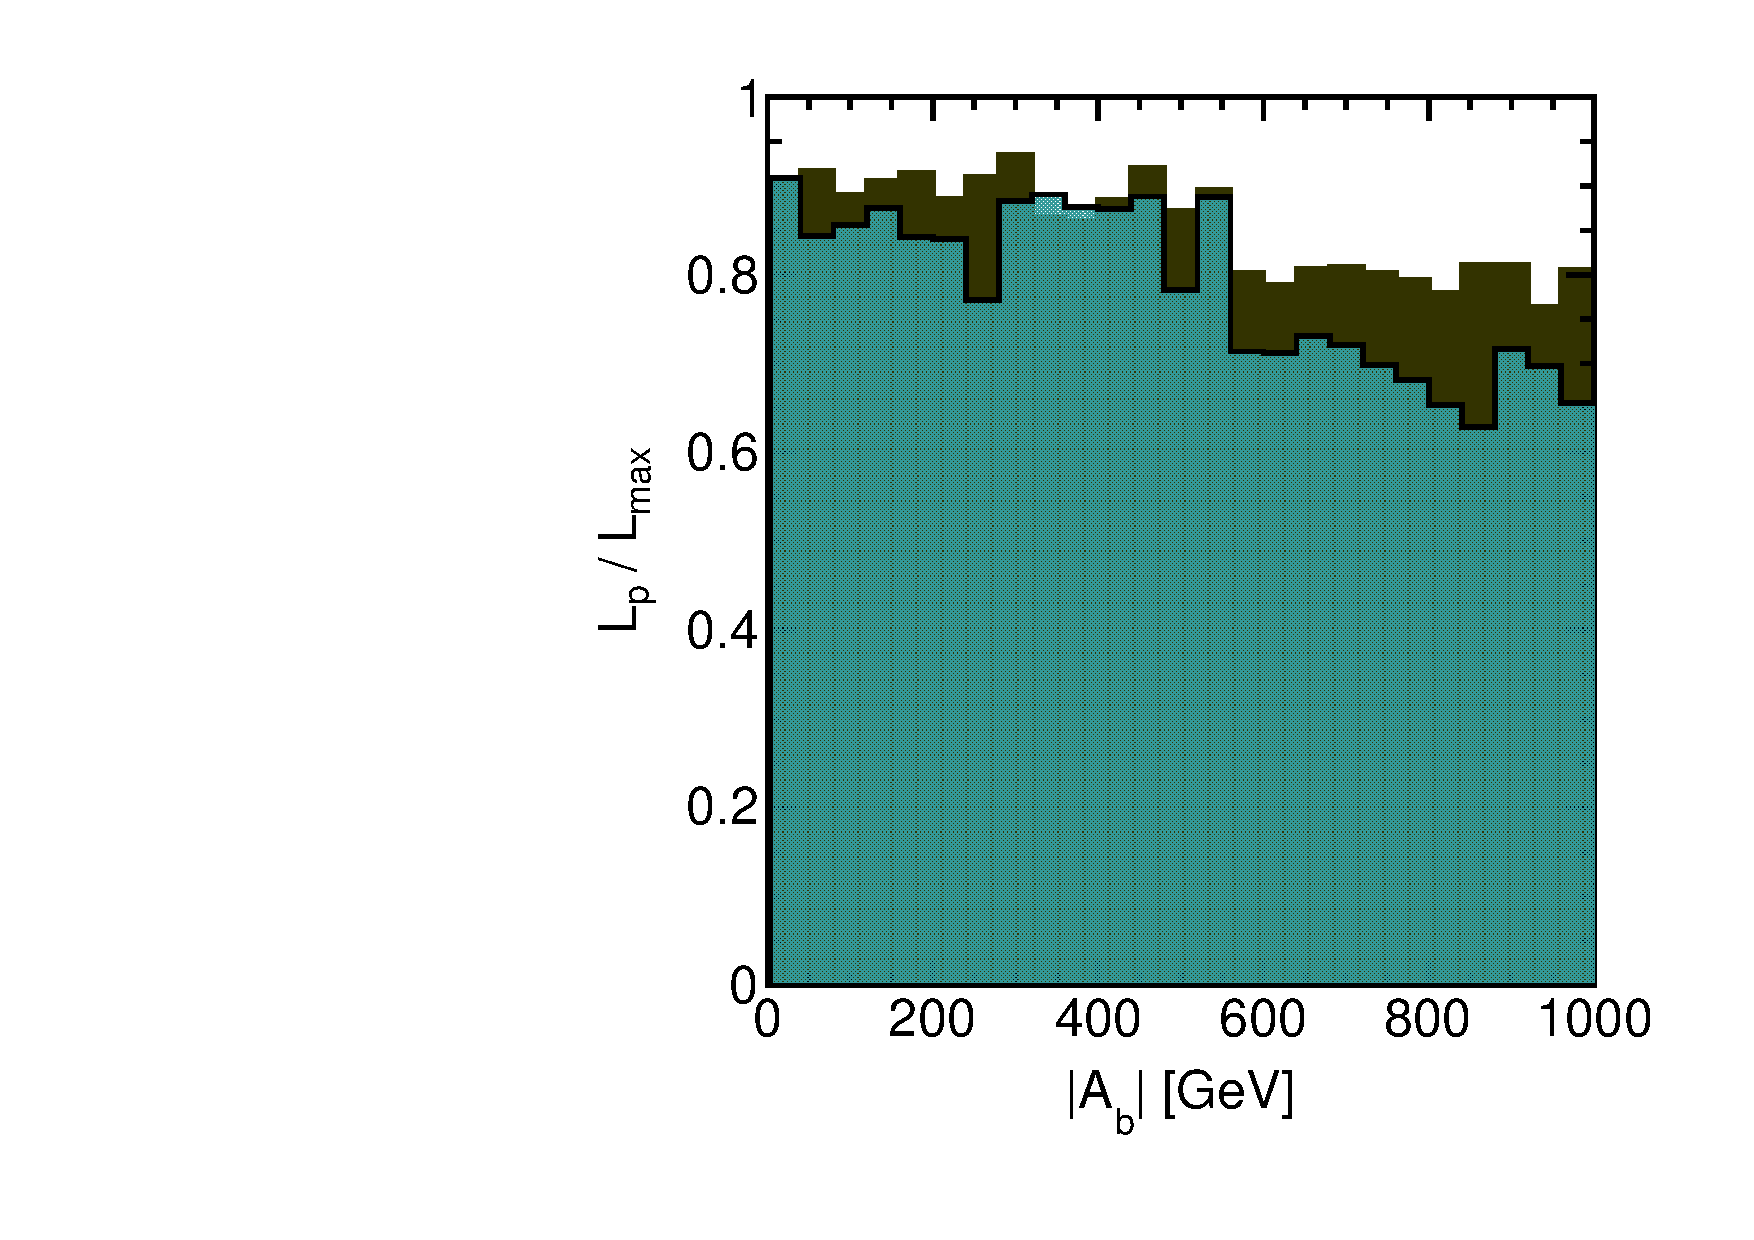
\includegraphics[height=5.5cm]{figs/fig_A_b.pdf} \\
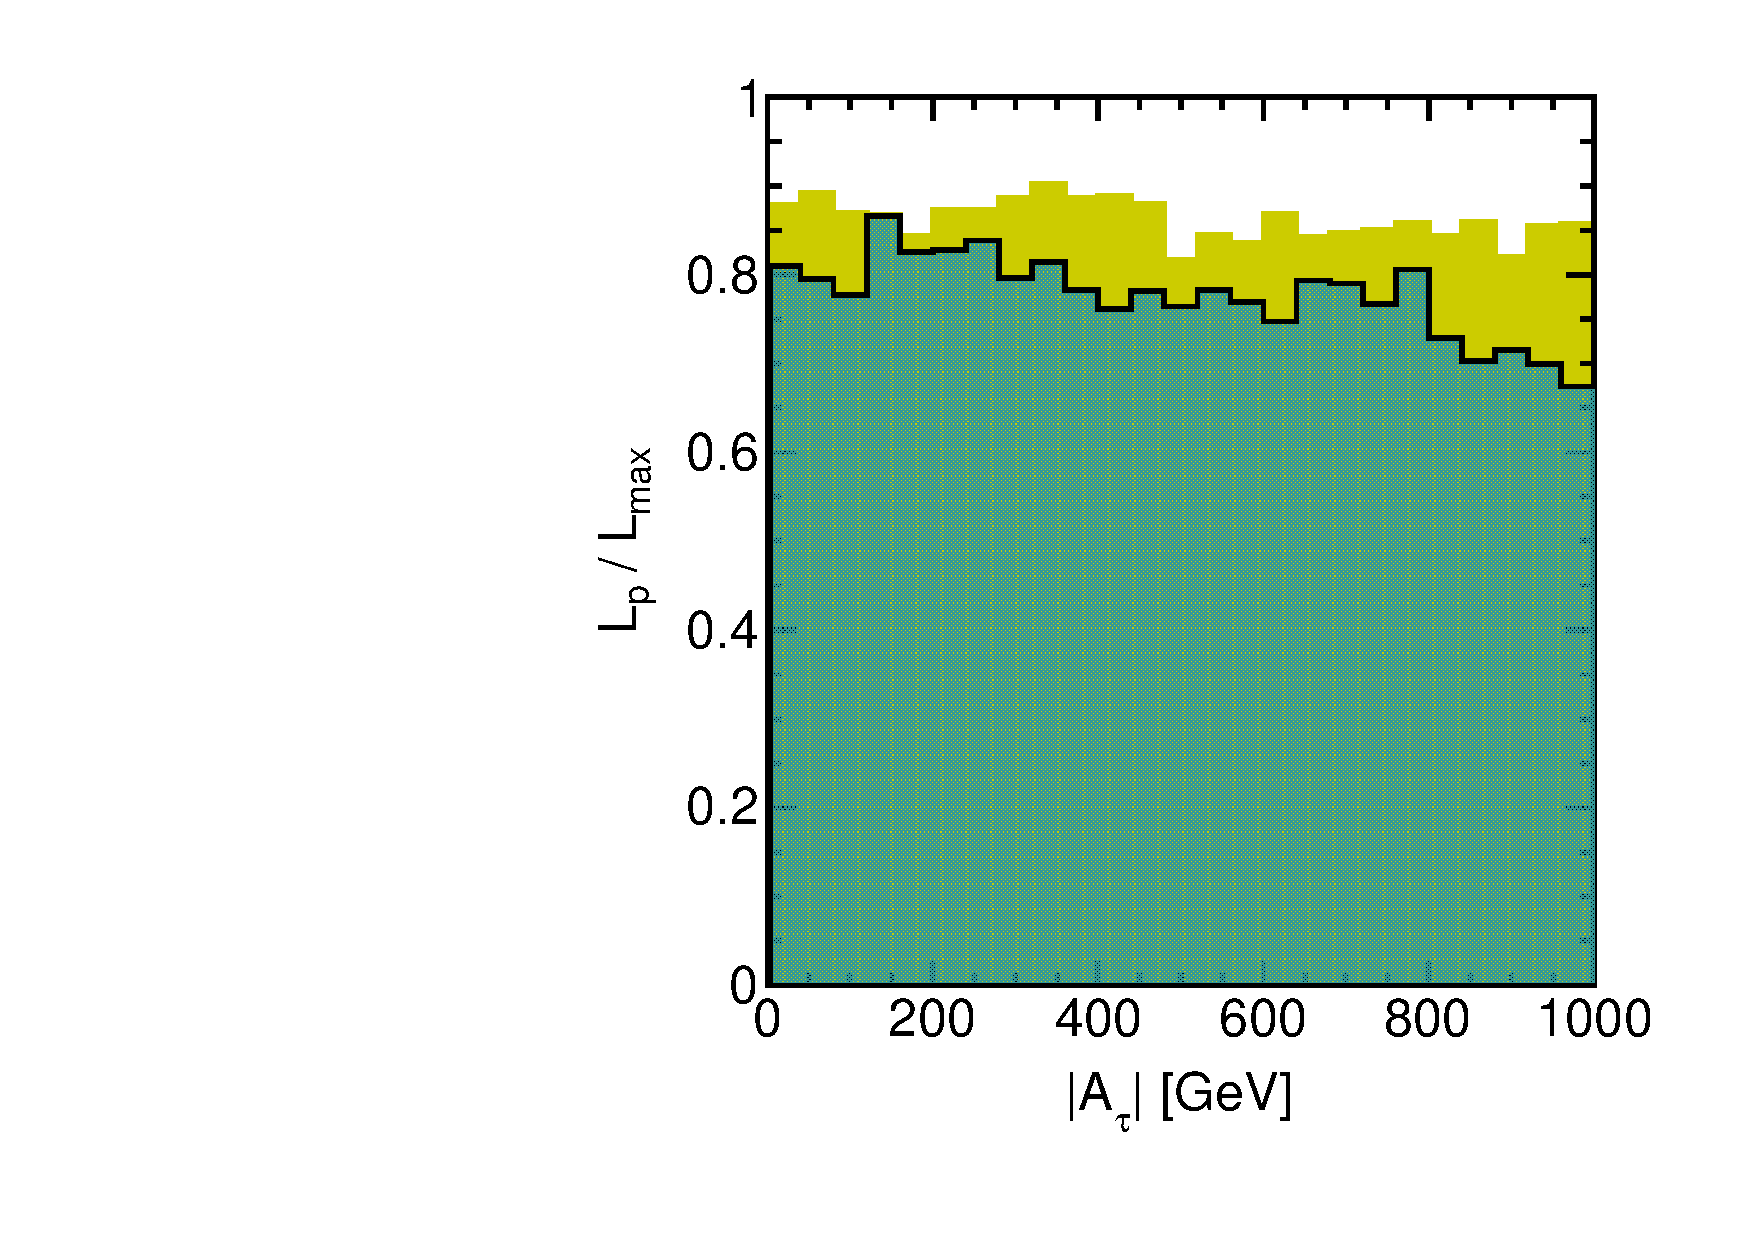
\includegraphics[height=5.5cm]{figs/fig_A_tau.pdf}
\caption{Ratios of profile likelihood $L_p$ to maximum likelihood $L_{max}$ shown for trilinear couplings at SUSY scale.  The colored and shaded histograms show the distributions before and after the inclusion of the CMS results.}
\label{fig:LRwcms_A}
\end{center}
\end{figure}

\begin{figure}[htbp]
\begin{center}
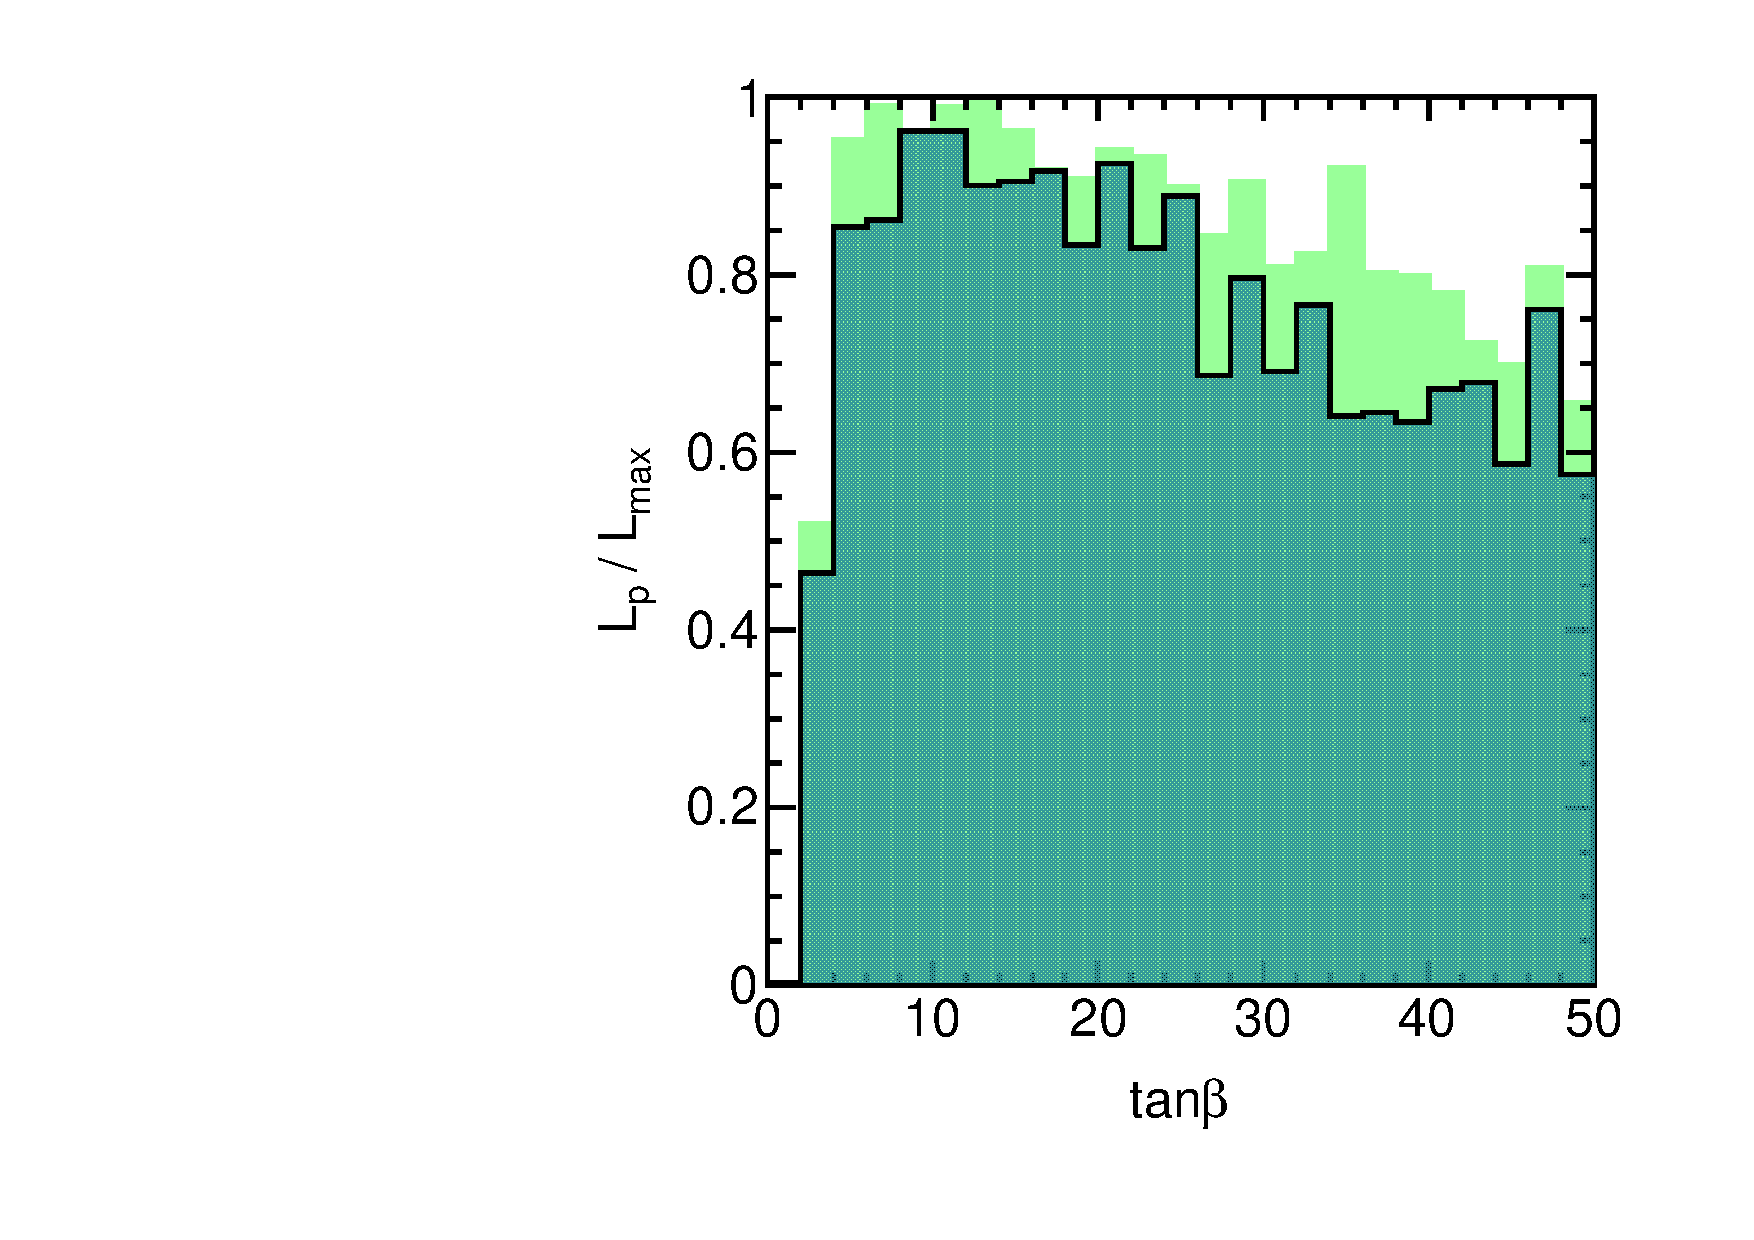
\includegraphics[height=5.5cm]{figs/fig_tanbeta.pdf} 
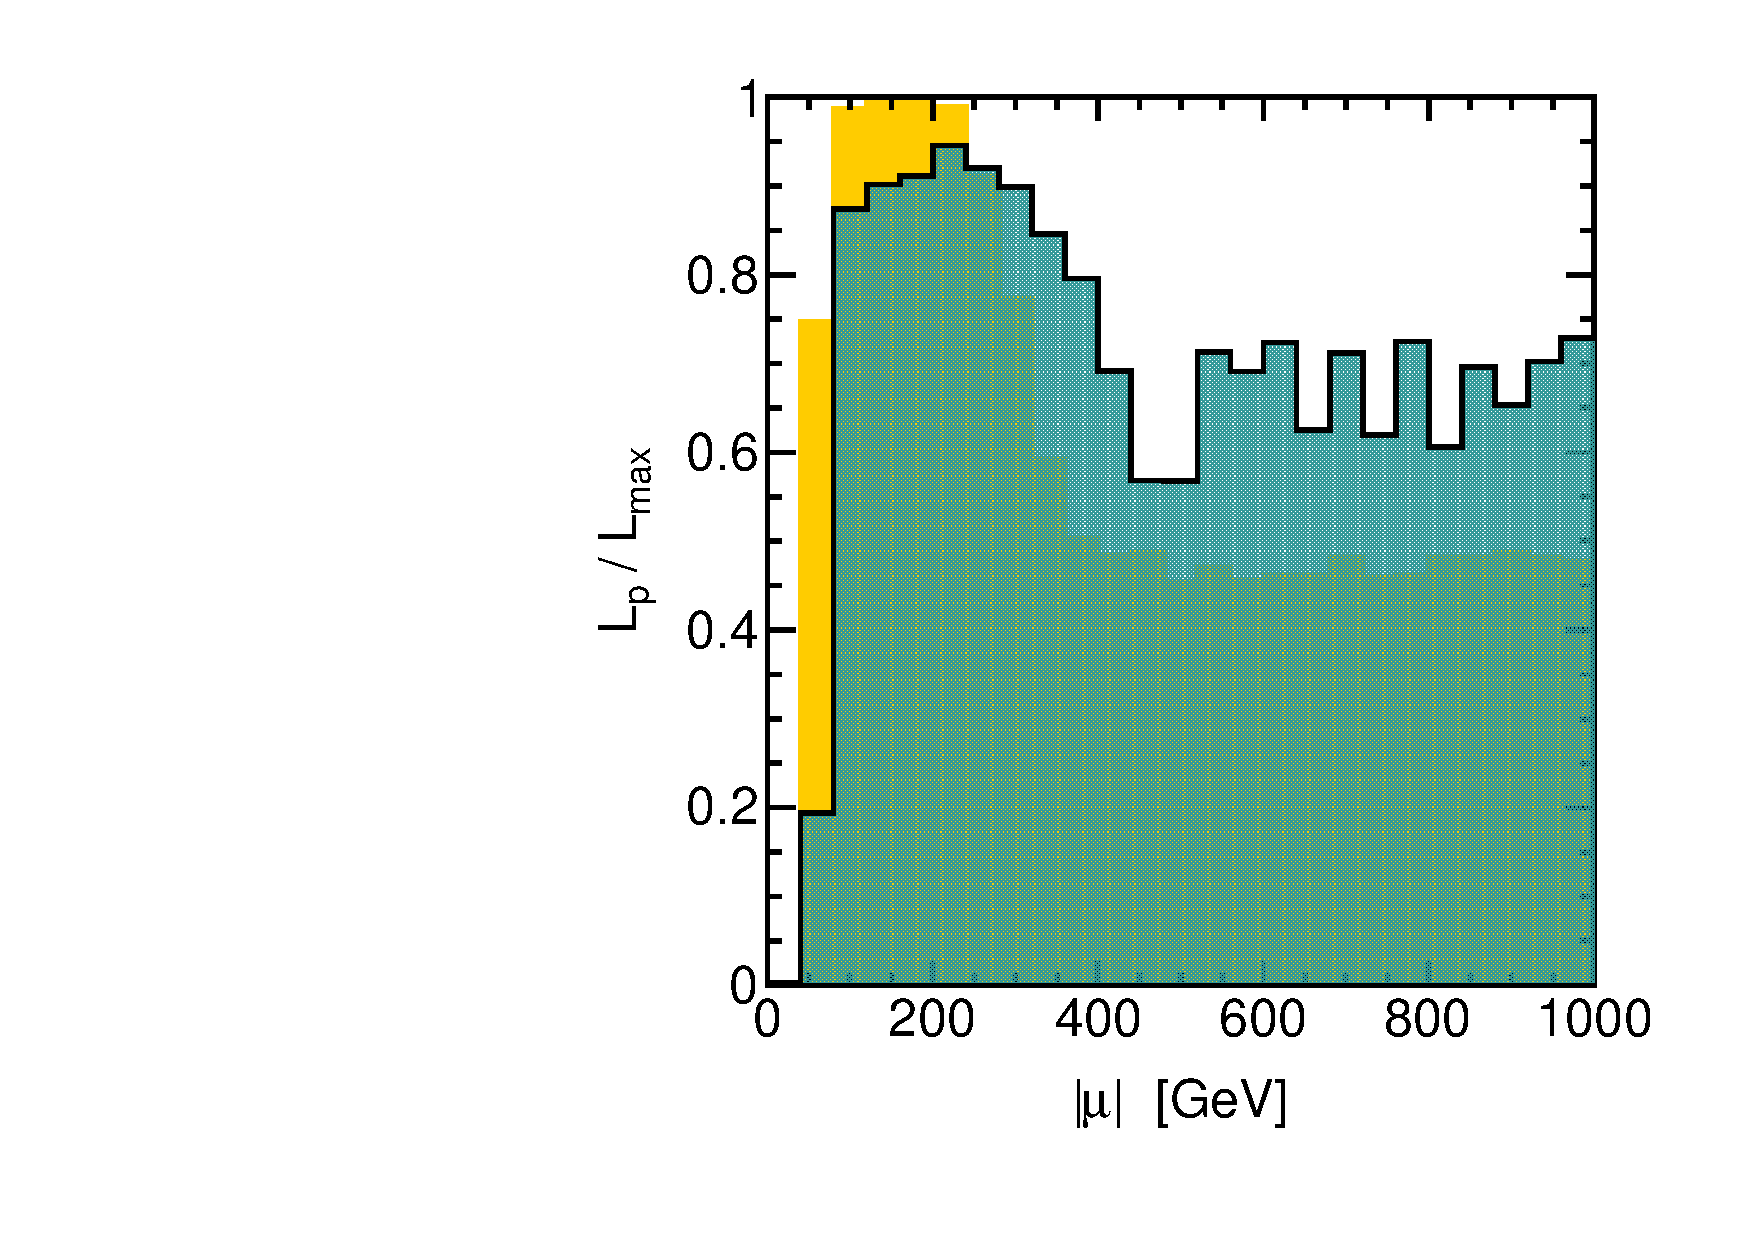
\includegraphics[height=5.5cm]{figs/fig_mu.pdf} 
\caption{Ratios of profile likelihood $L_p$ to maximum likelihood $L_{max}$ shown for $\tan\beta$ and $\mu$ parameter at SUSY scale.  The colored and shaded histograms show the distributions before and after the inclusion of the CMS results.}
\label{fig:LRwcms_tbmu}
\end{center}
\end{figure}



\begin{figure}[htbp]
\begin{center}
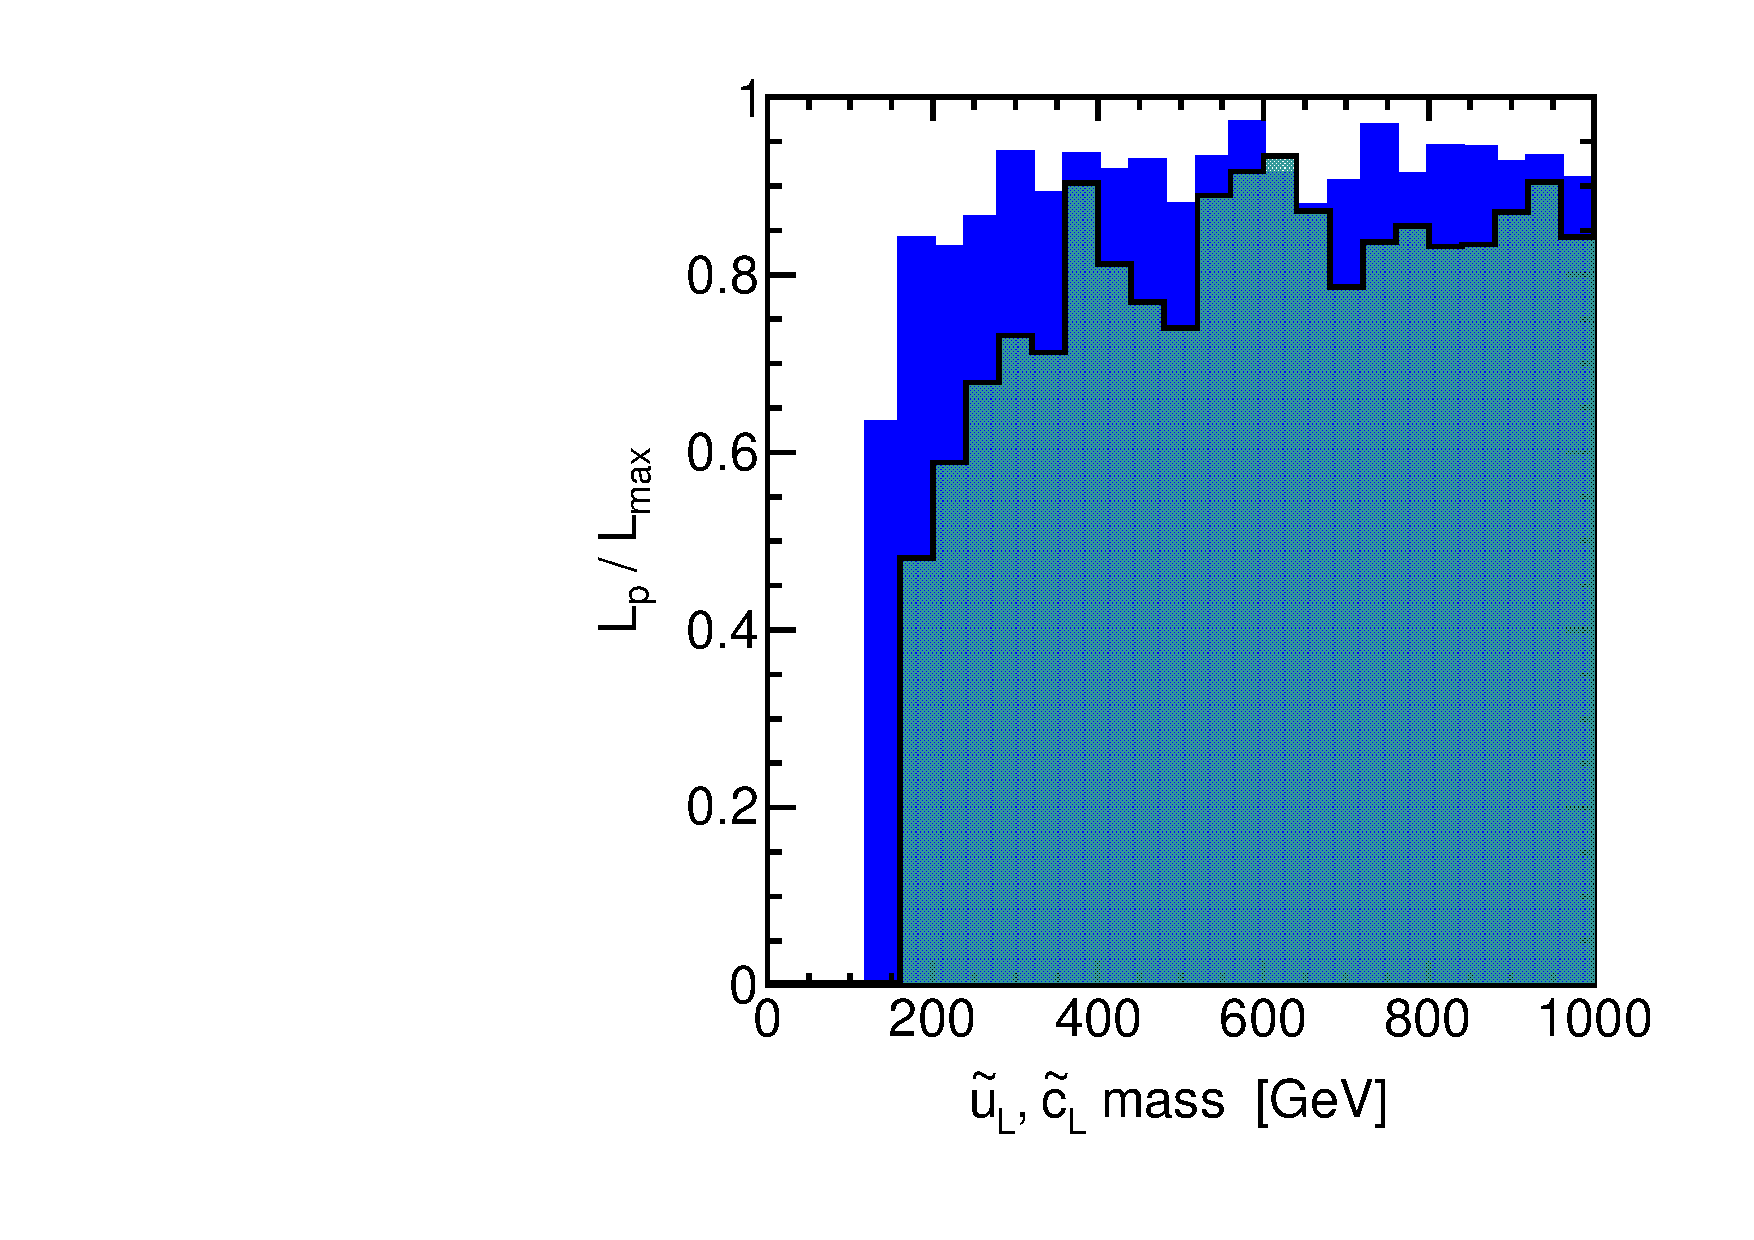
\includegraphics[height=5.5cm]{figs/fig_u_L.pdf} 
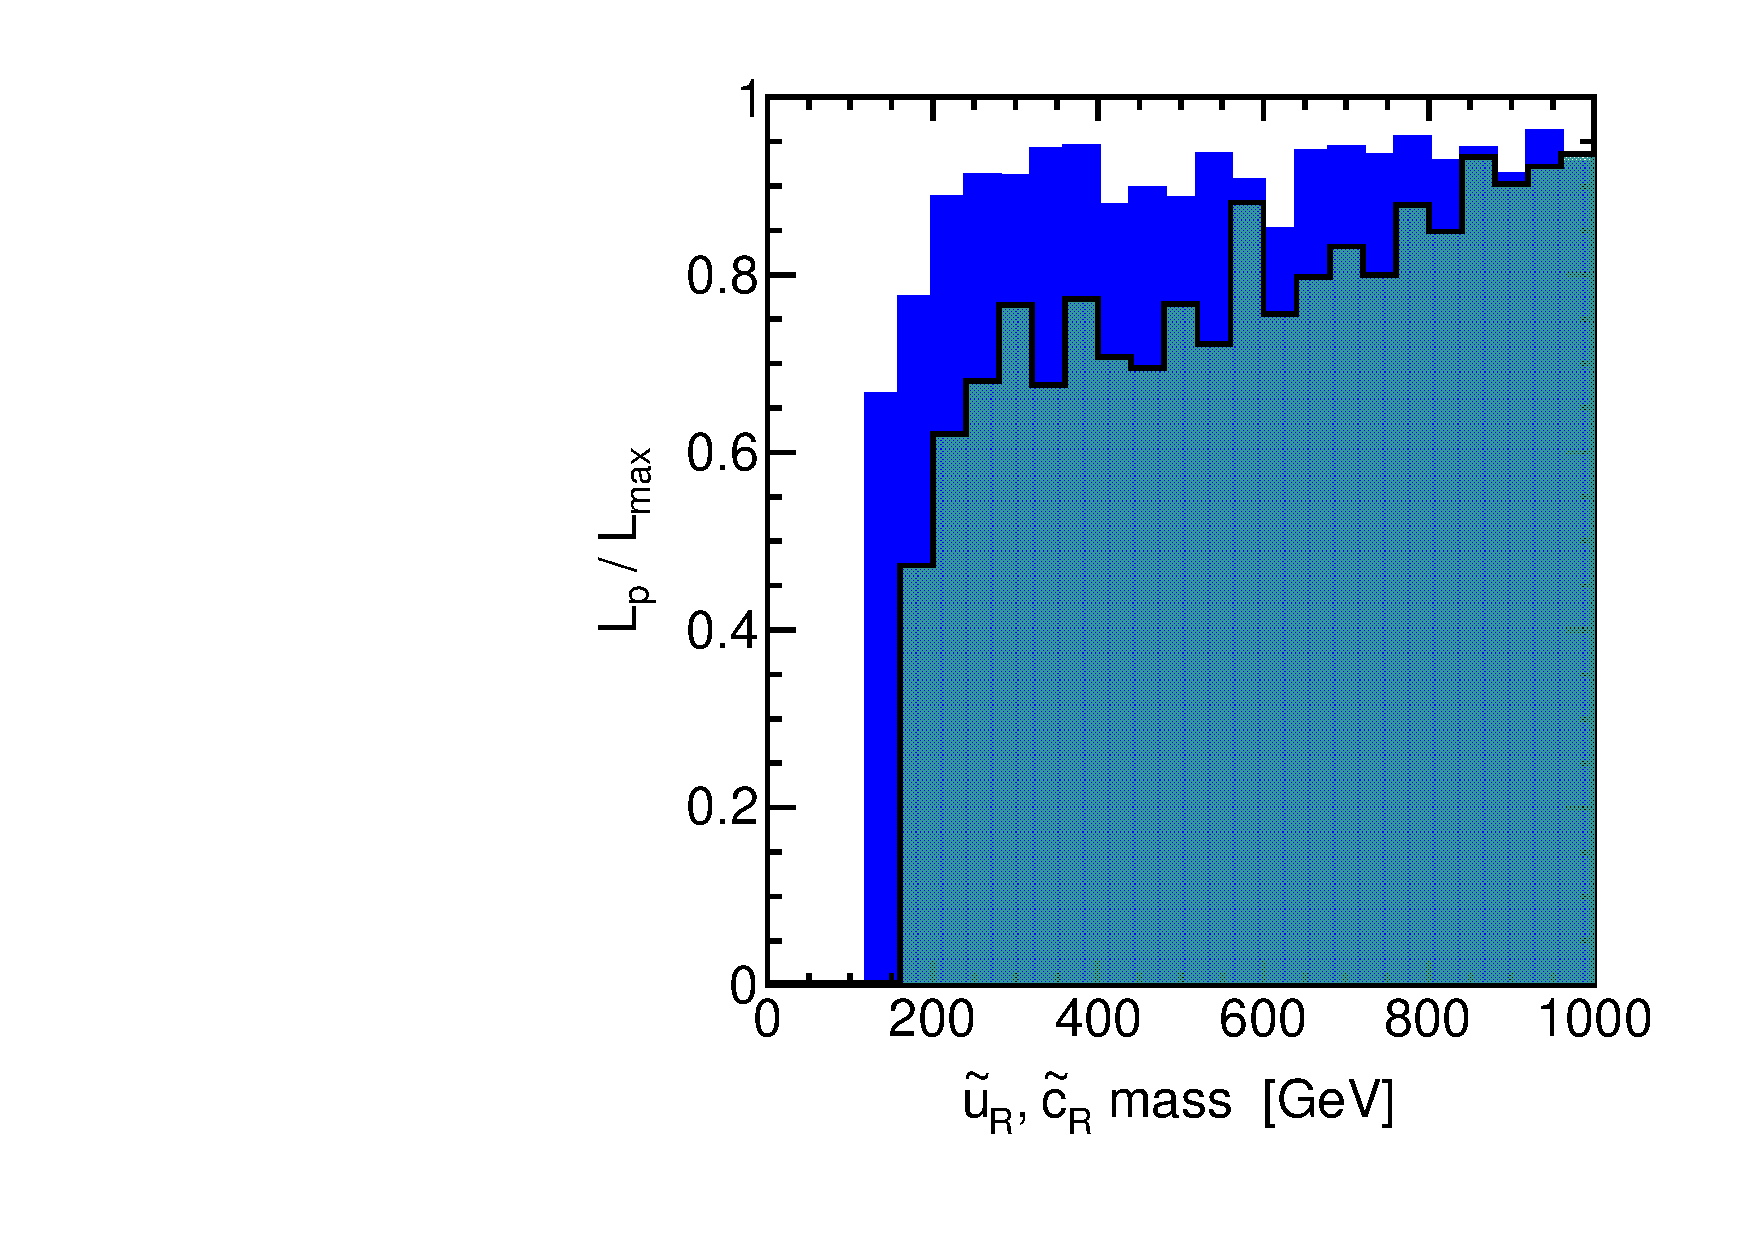
\includegraphics[height=5.5cm]{figs/fig_u_R.pdf} \\
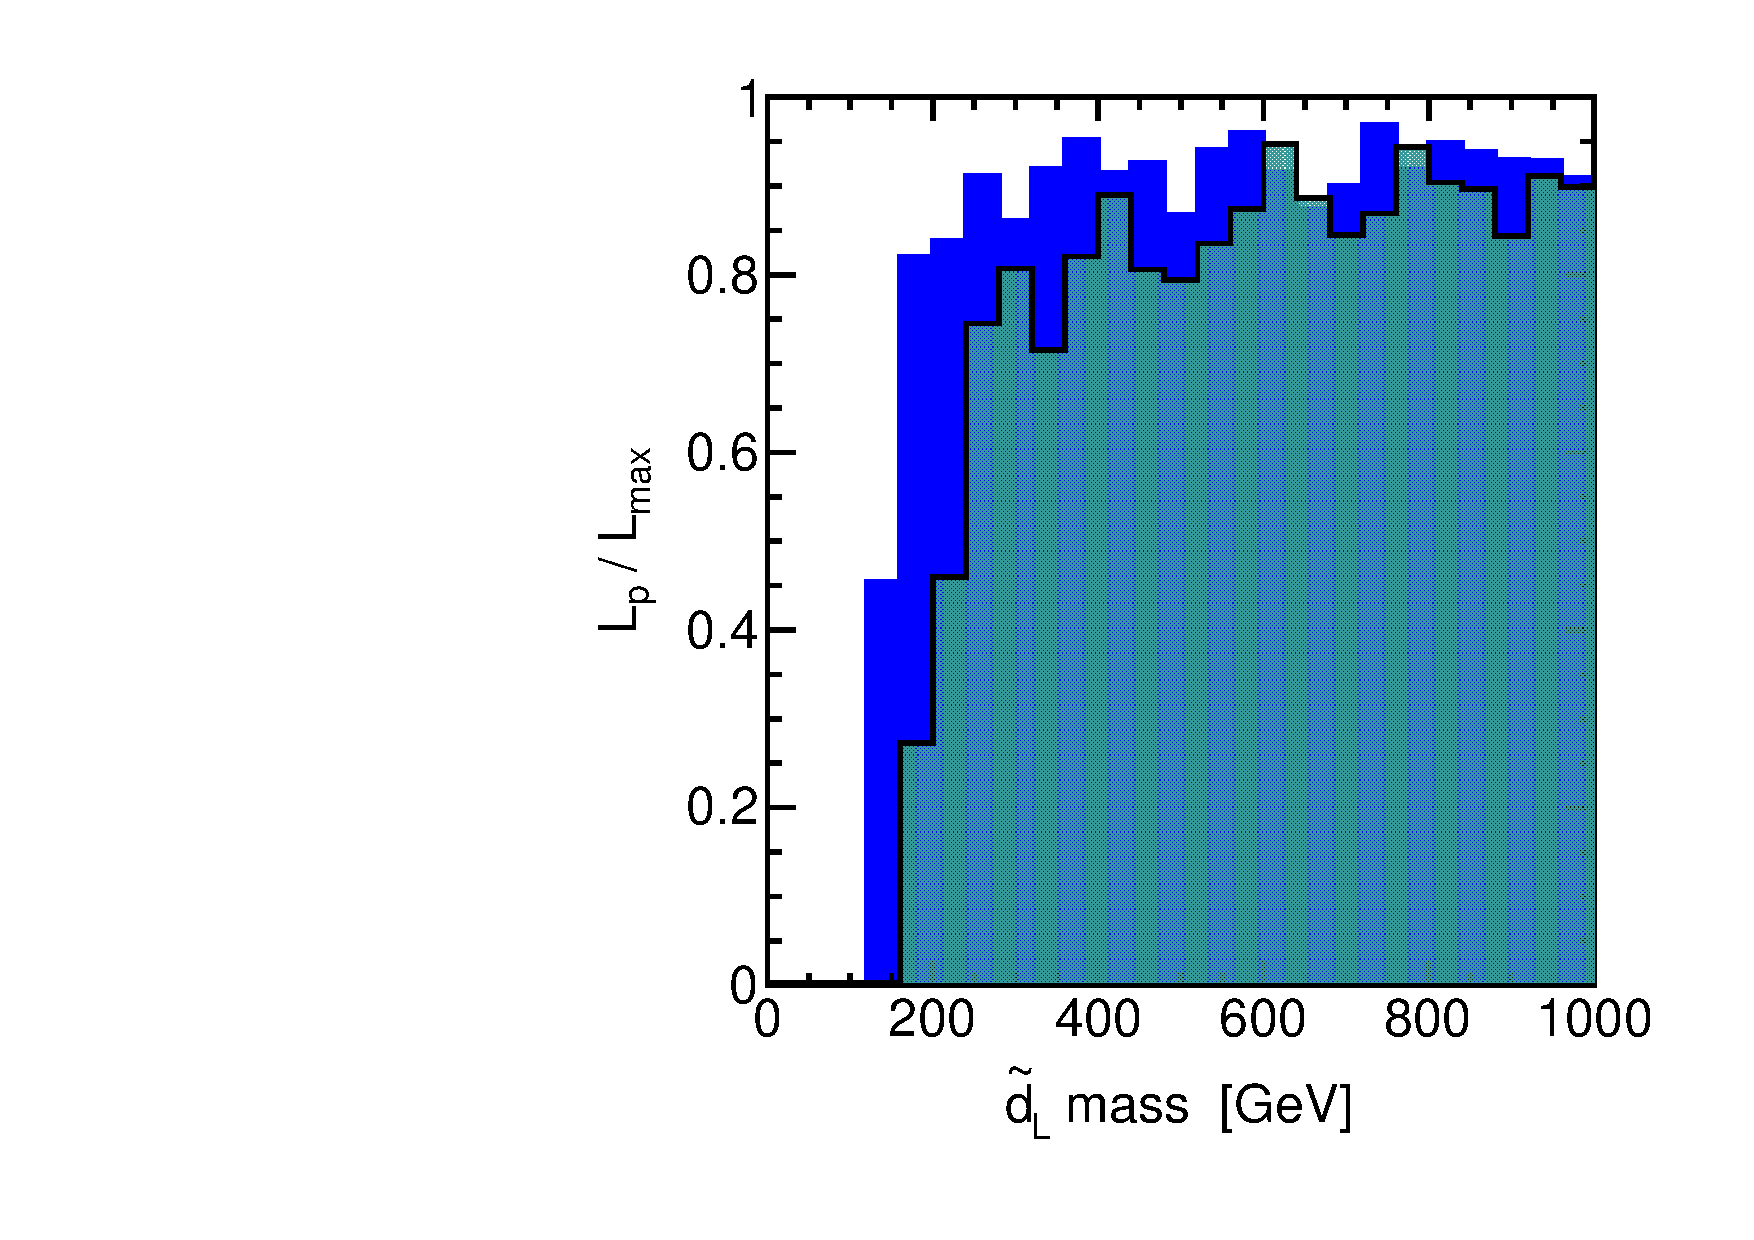
\includegraphics[height=5.5cm]{figs/fig_d_L.pdf} 
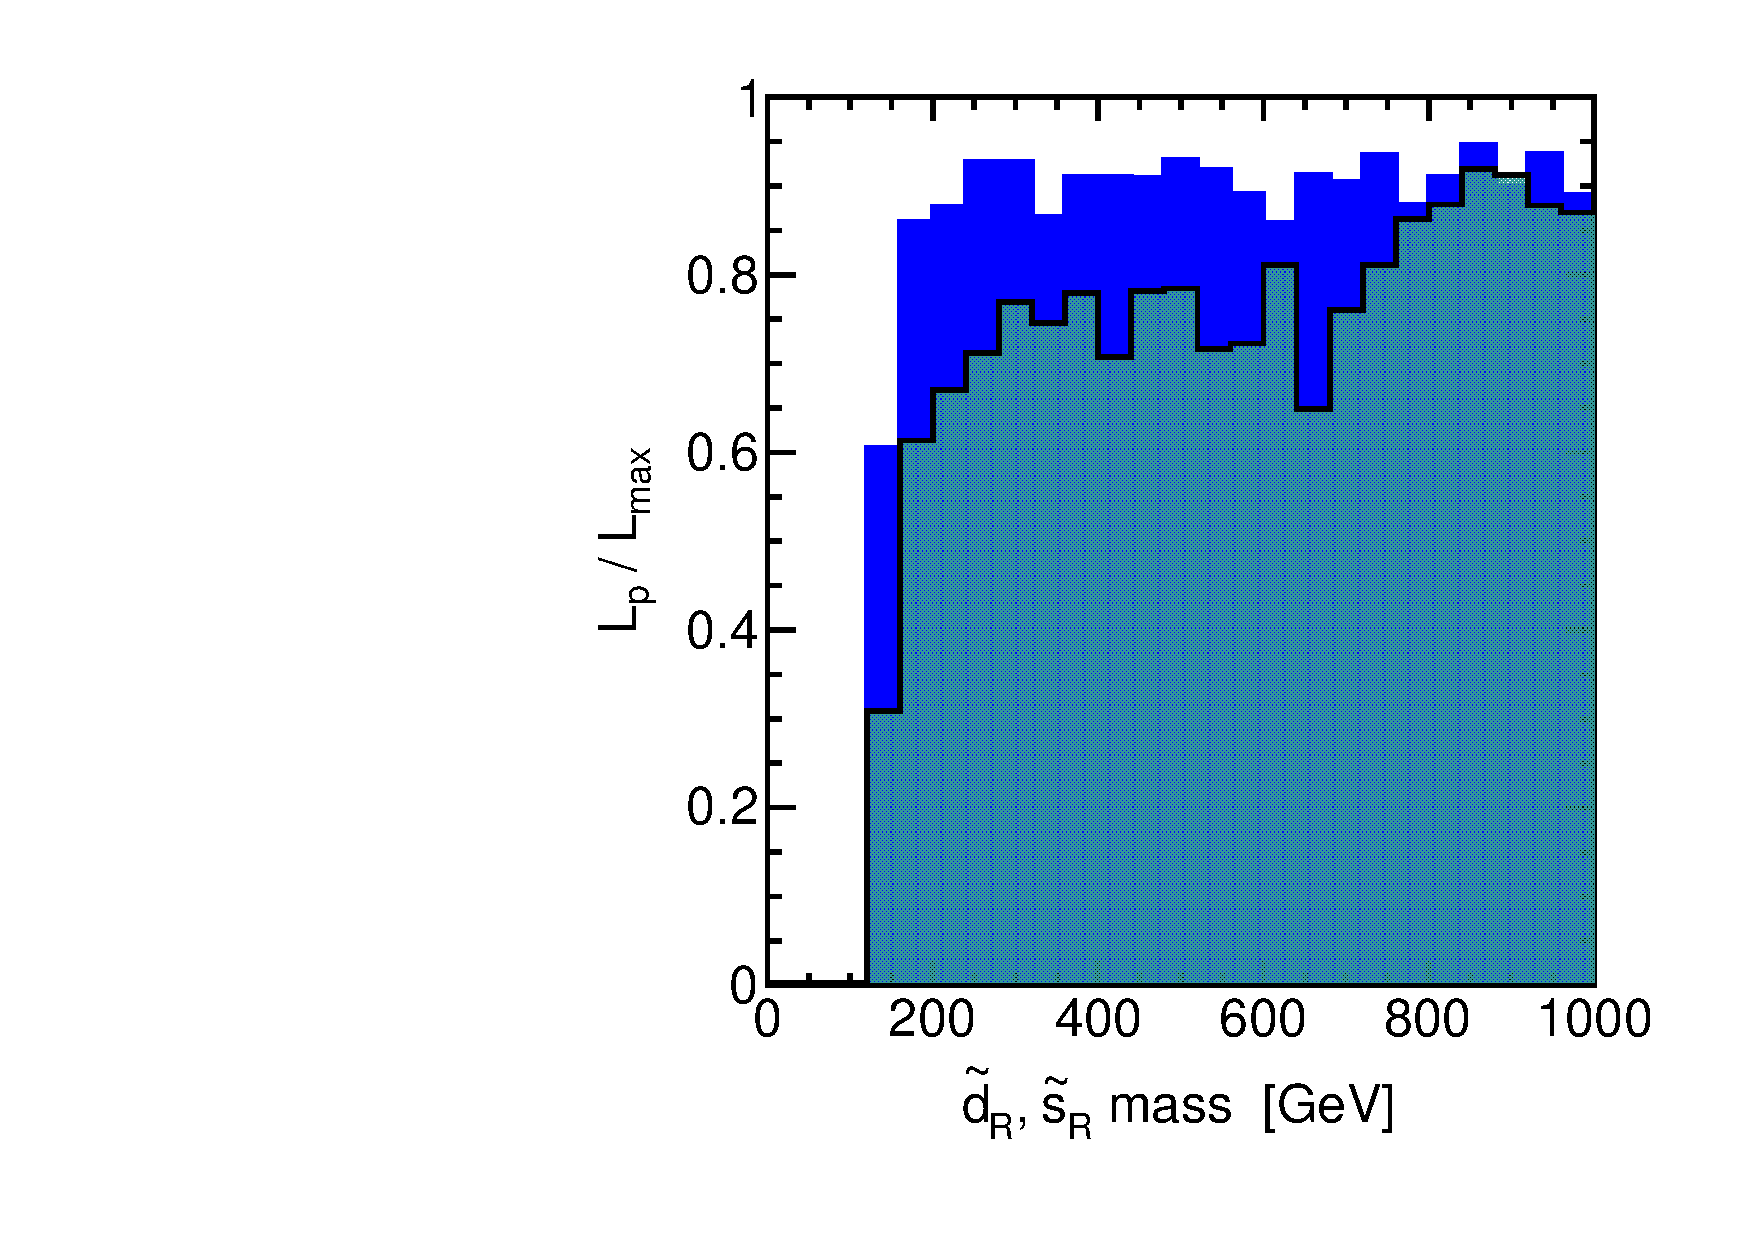
\includegraphics[height=5.5cm]{figs/fig_d_R.pdf} \\
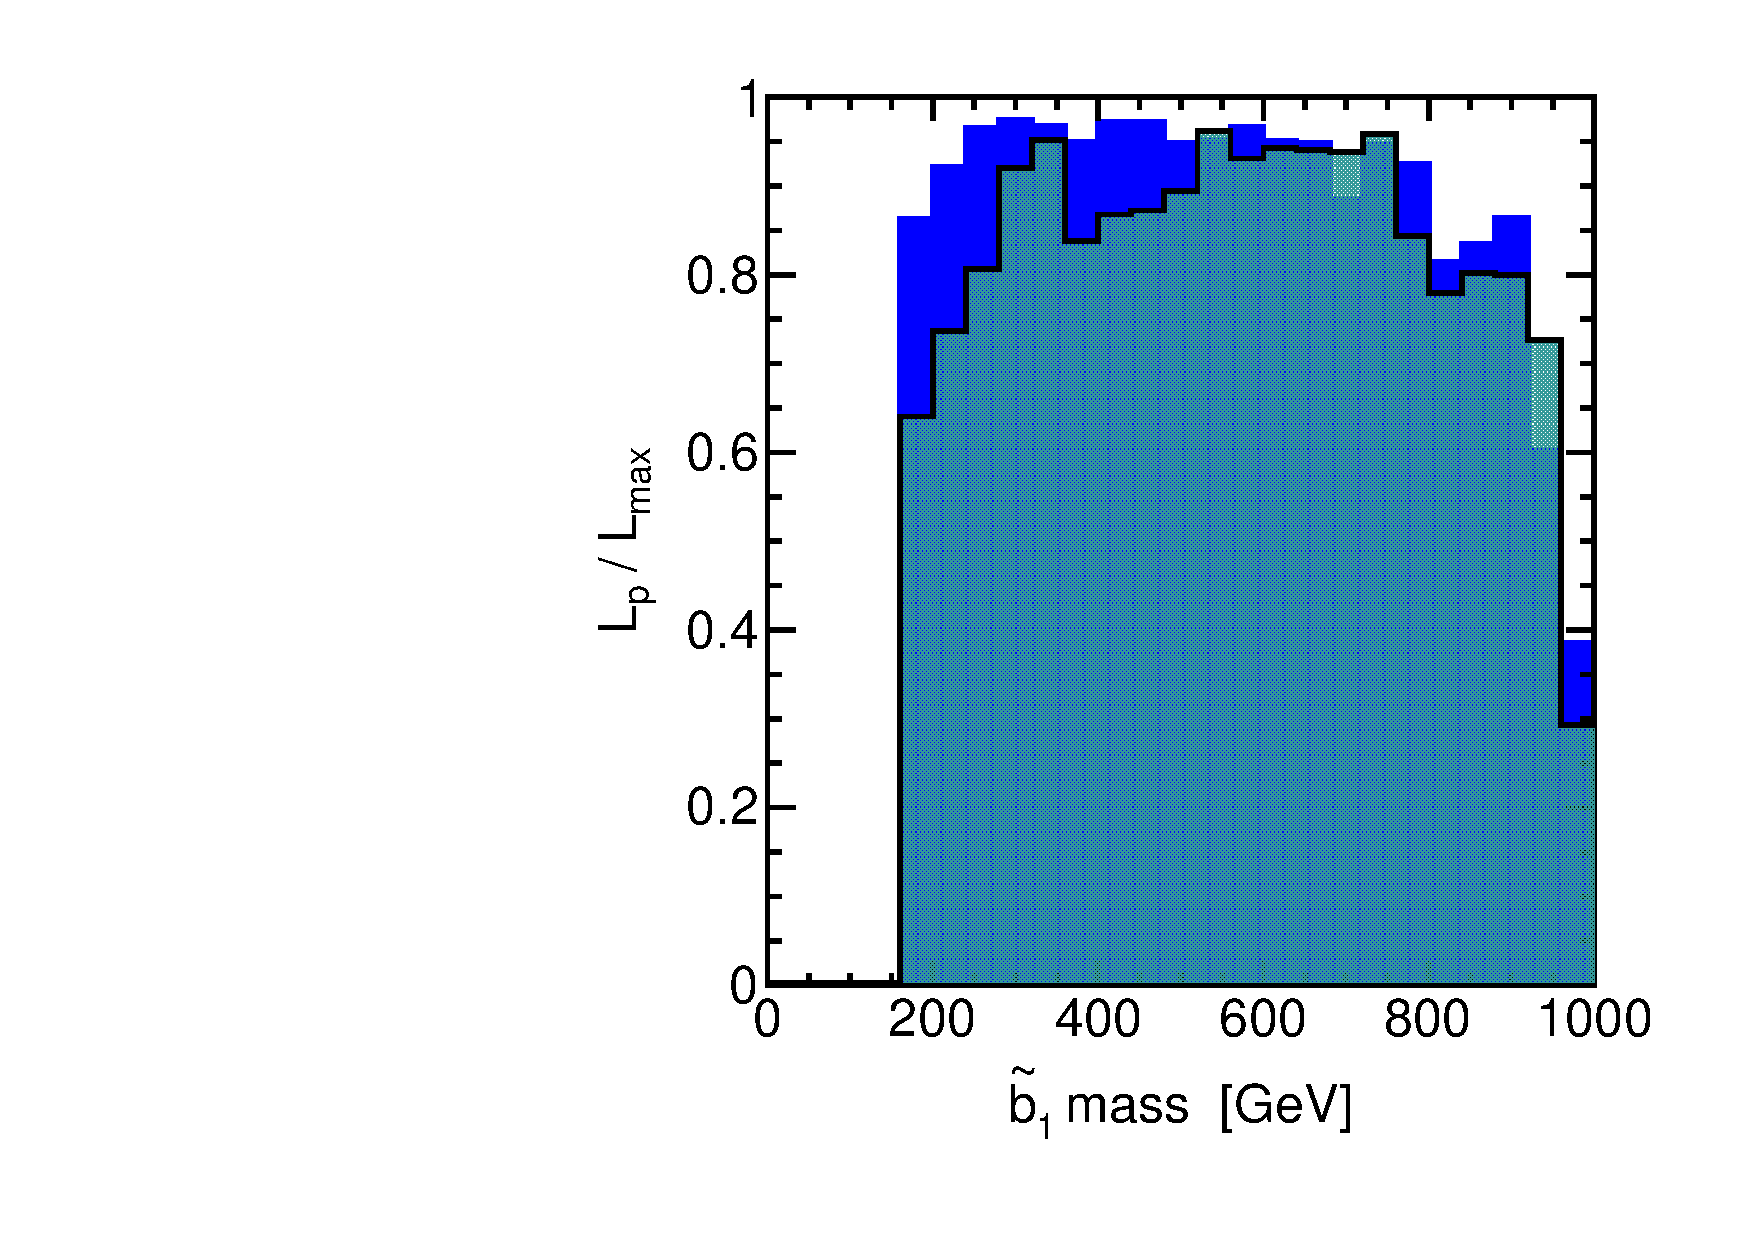
\includegraphics[height=5.5cm]{figs/fig_b_1.pdf} 
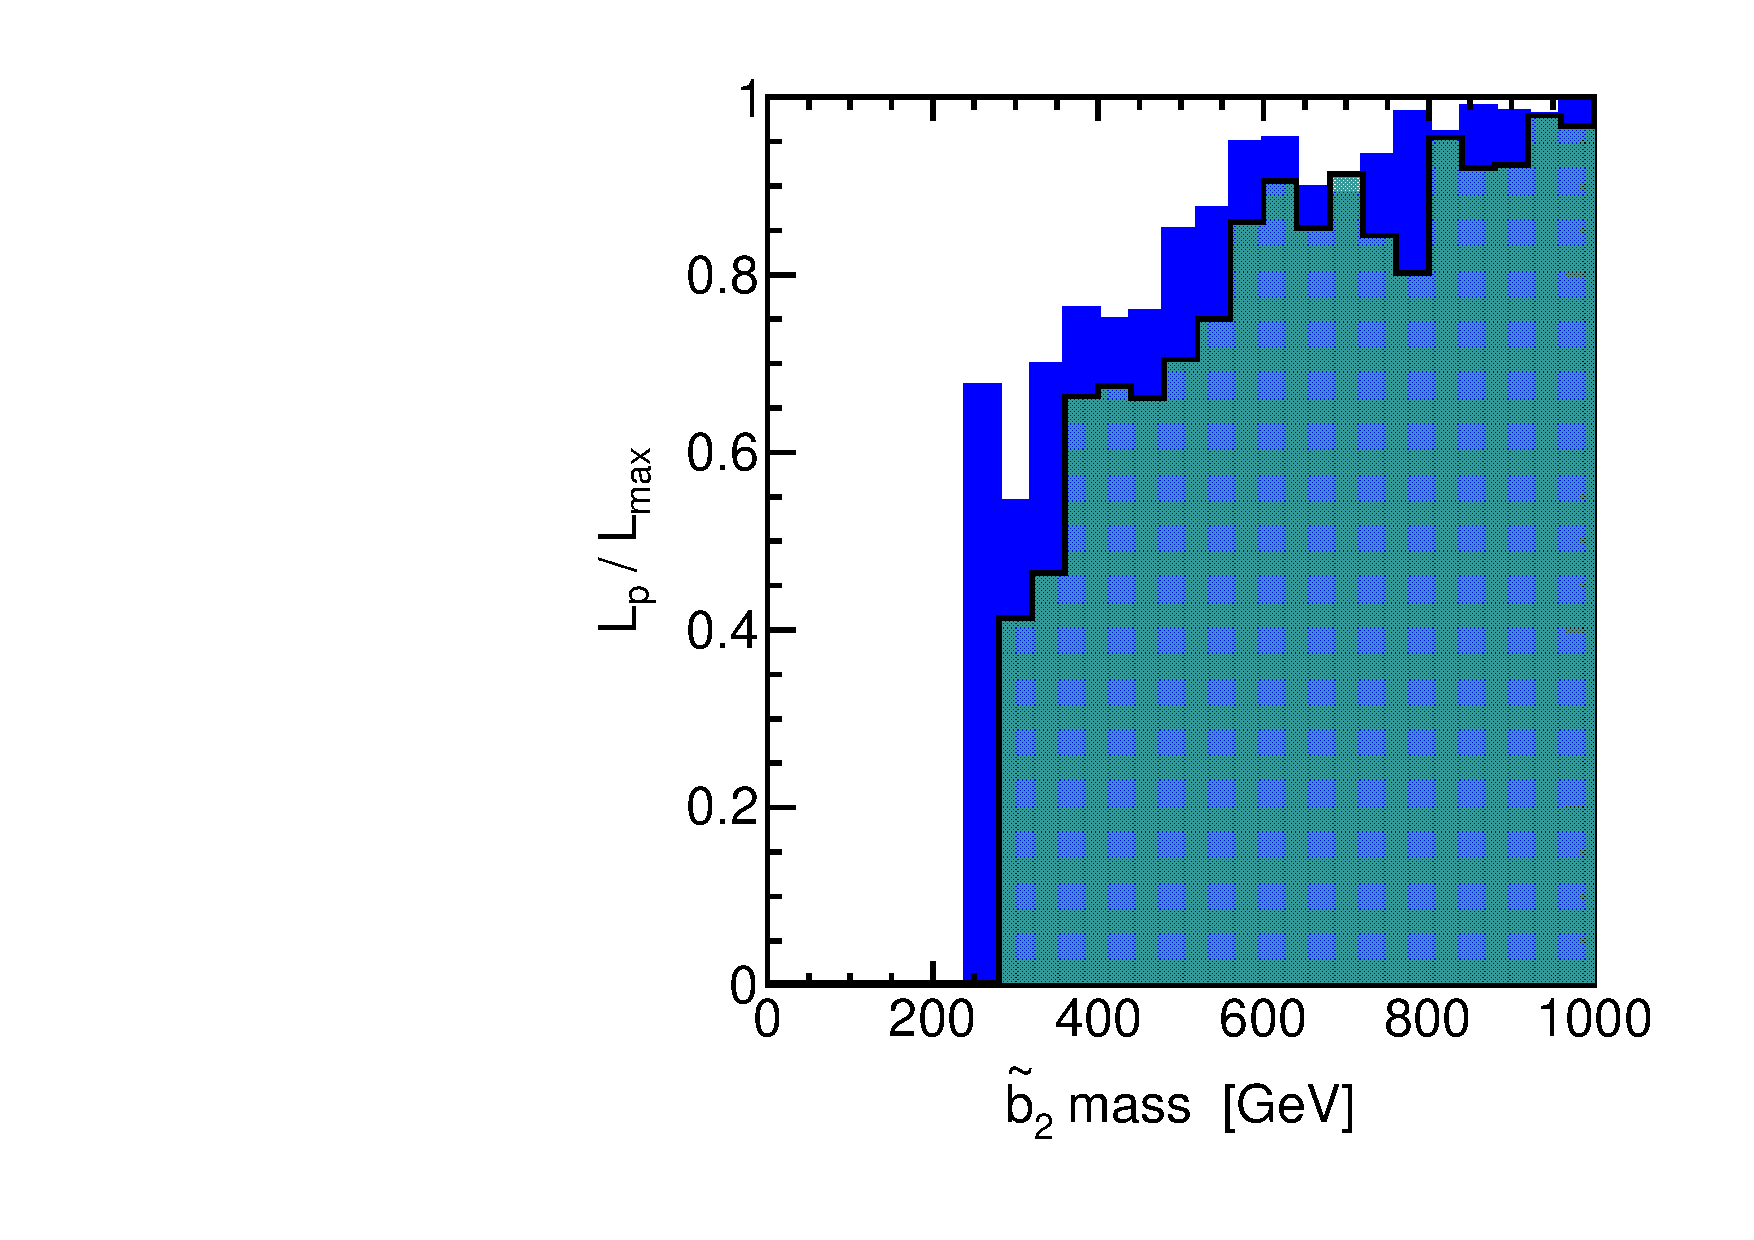
\includegraphics[height=5.5cm]{figs/fig_b_2.pdf} \\
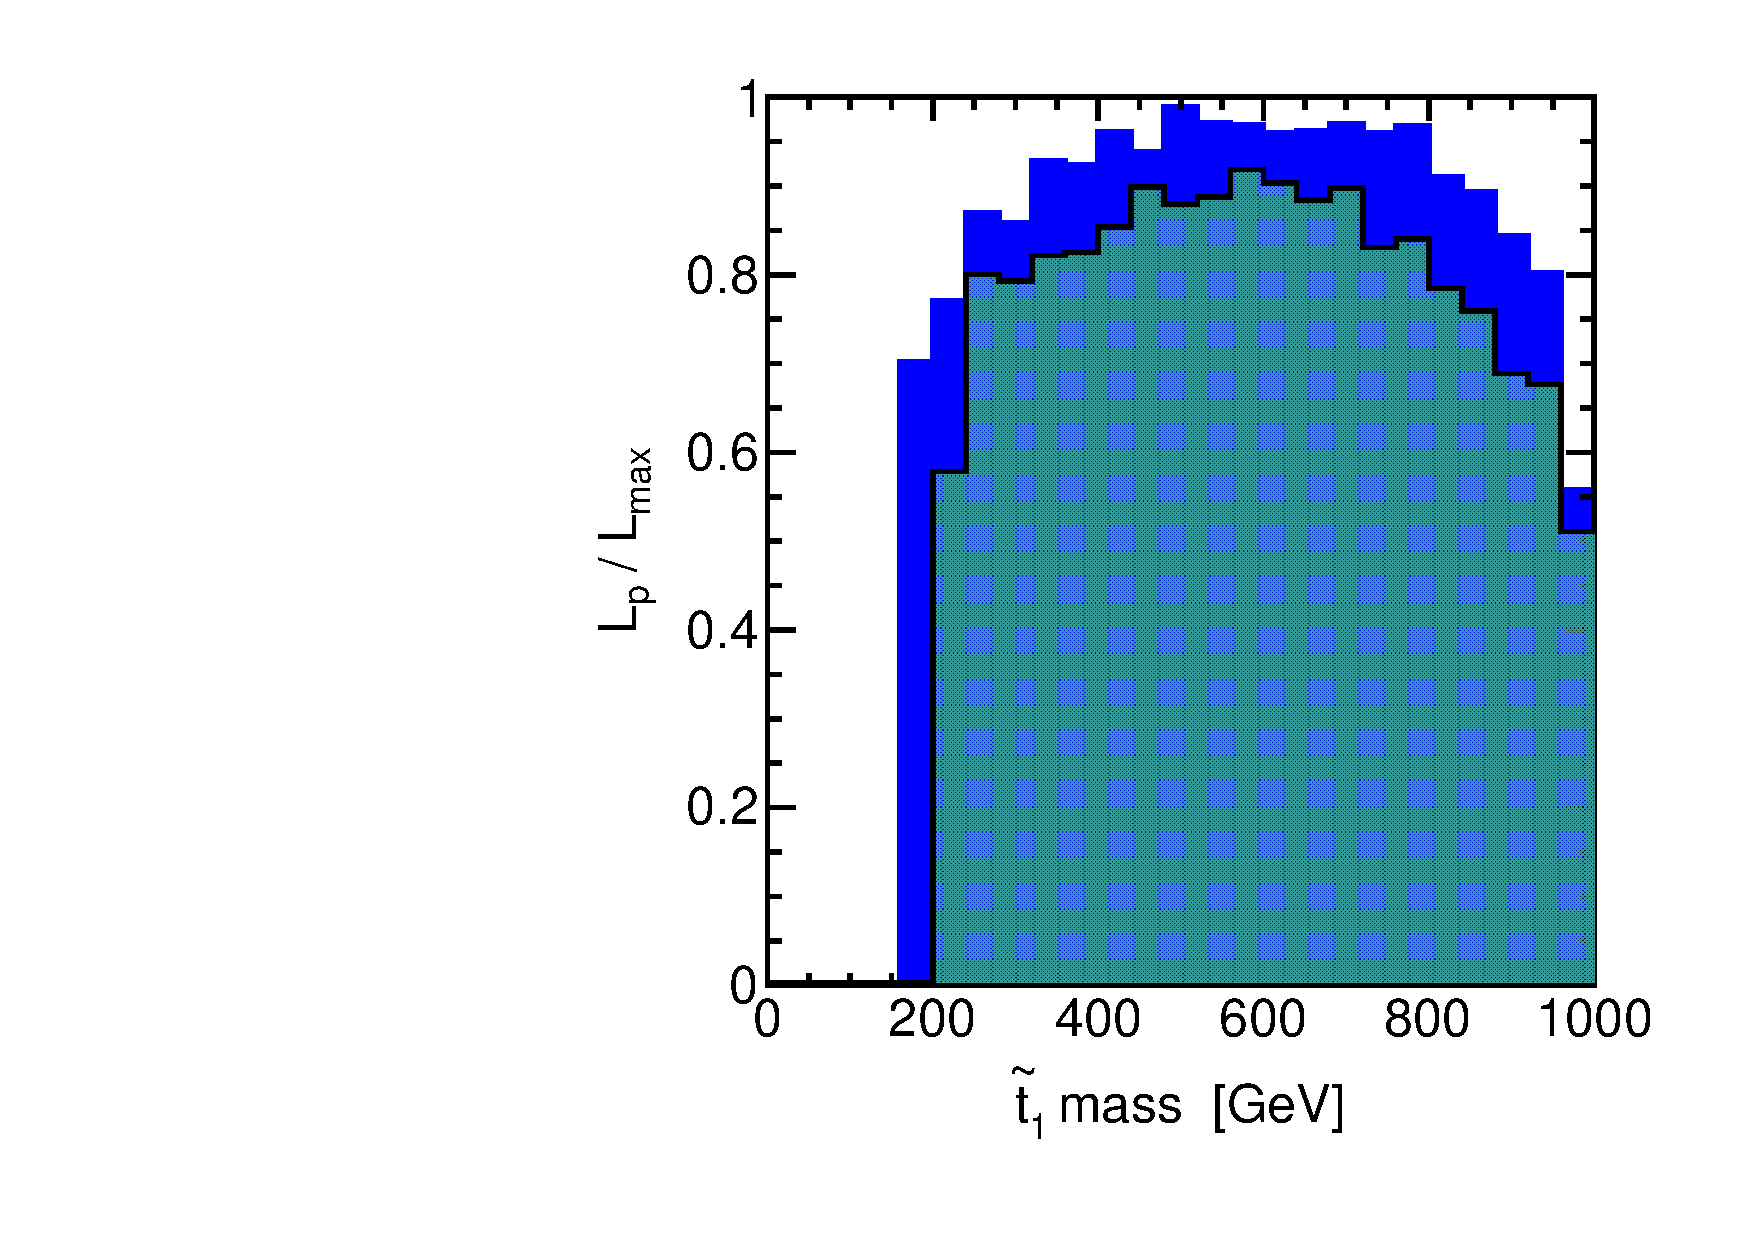
\includegraphics[height=5.5cm]{figs/fig_t_1.pdf} 
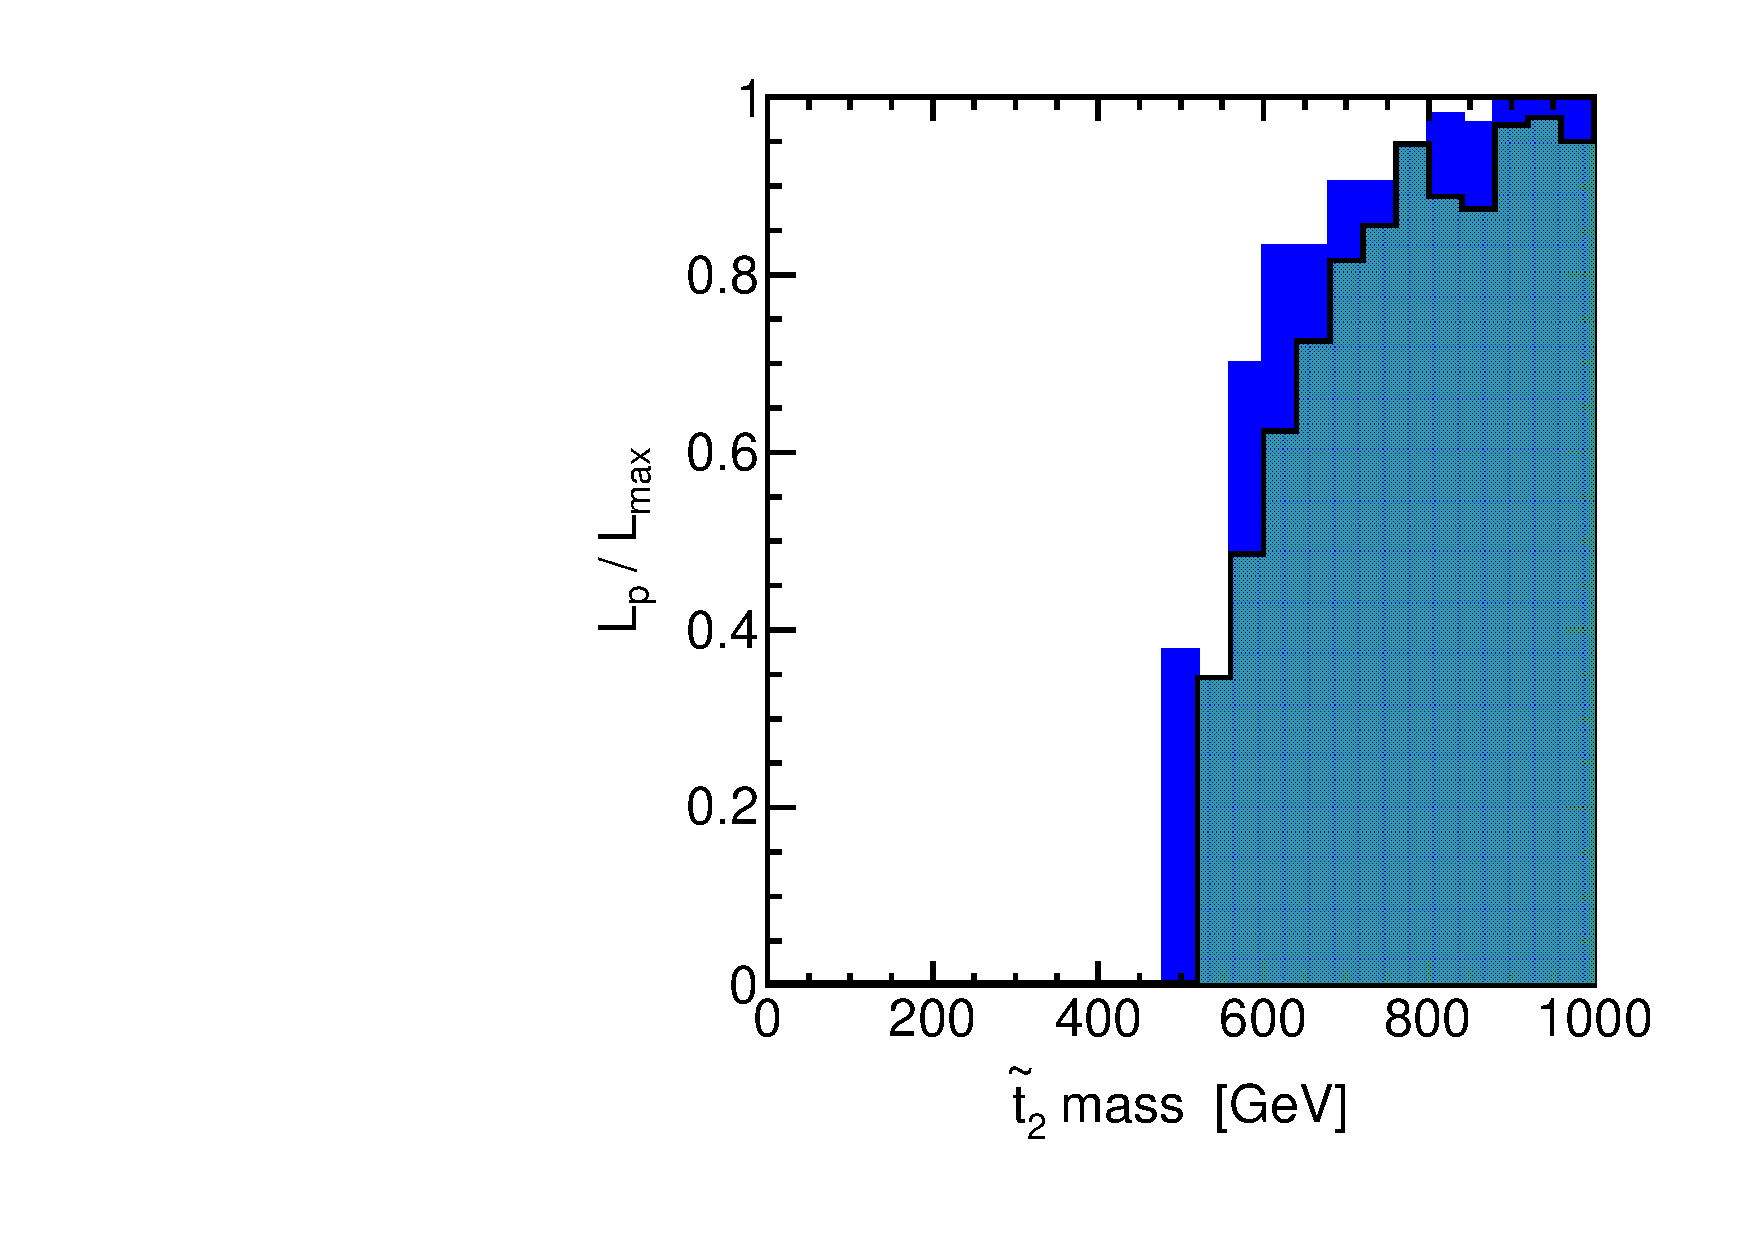
\includegraphics[height=5.5cm]{figs/fig_t_2.pdf} \\
\caption{Ratios of profile likelihood $L_p$ to maximum likelihood $L_{max}$ shown for squark masses.  The colored and shaded histograms show the distributions before and after the inclusion of the CMS results.}
\label{fig:LRwcms_sq}
\end{center}
\end{figure}


\begin{figure}[htbp]
\begin{center}
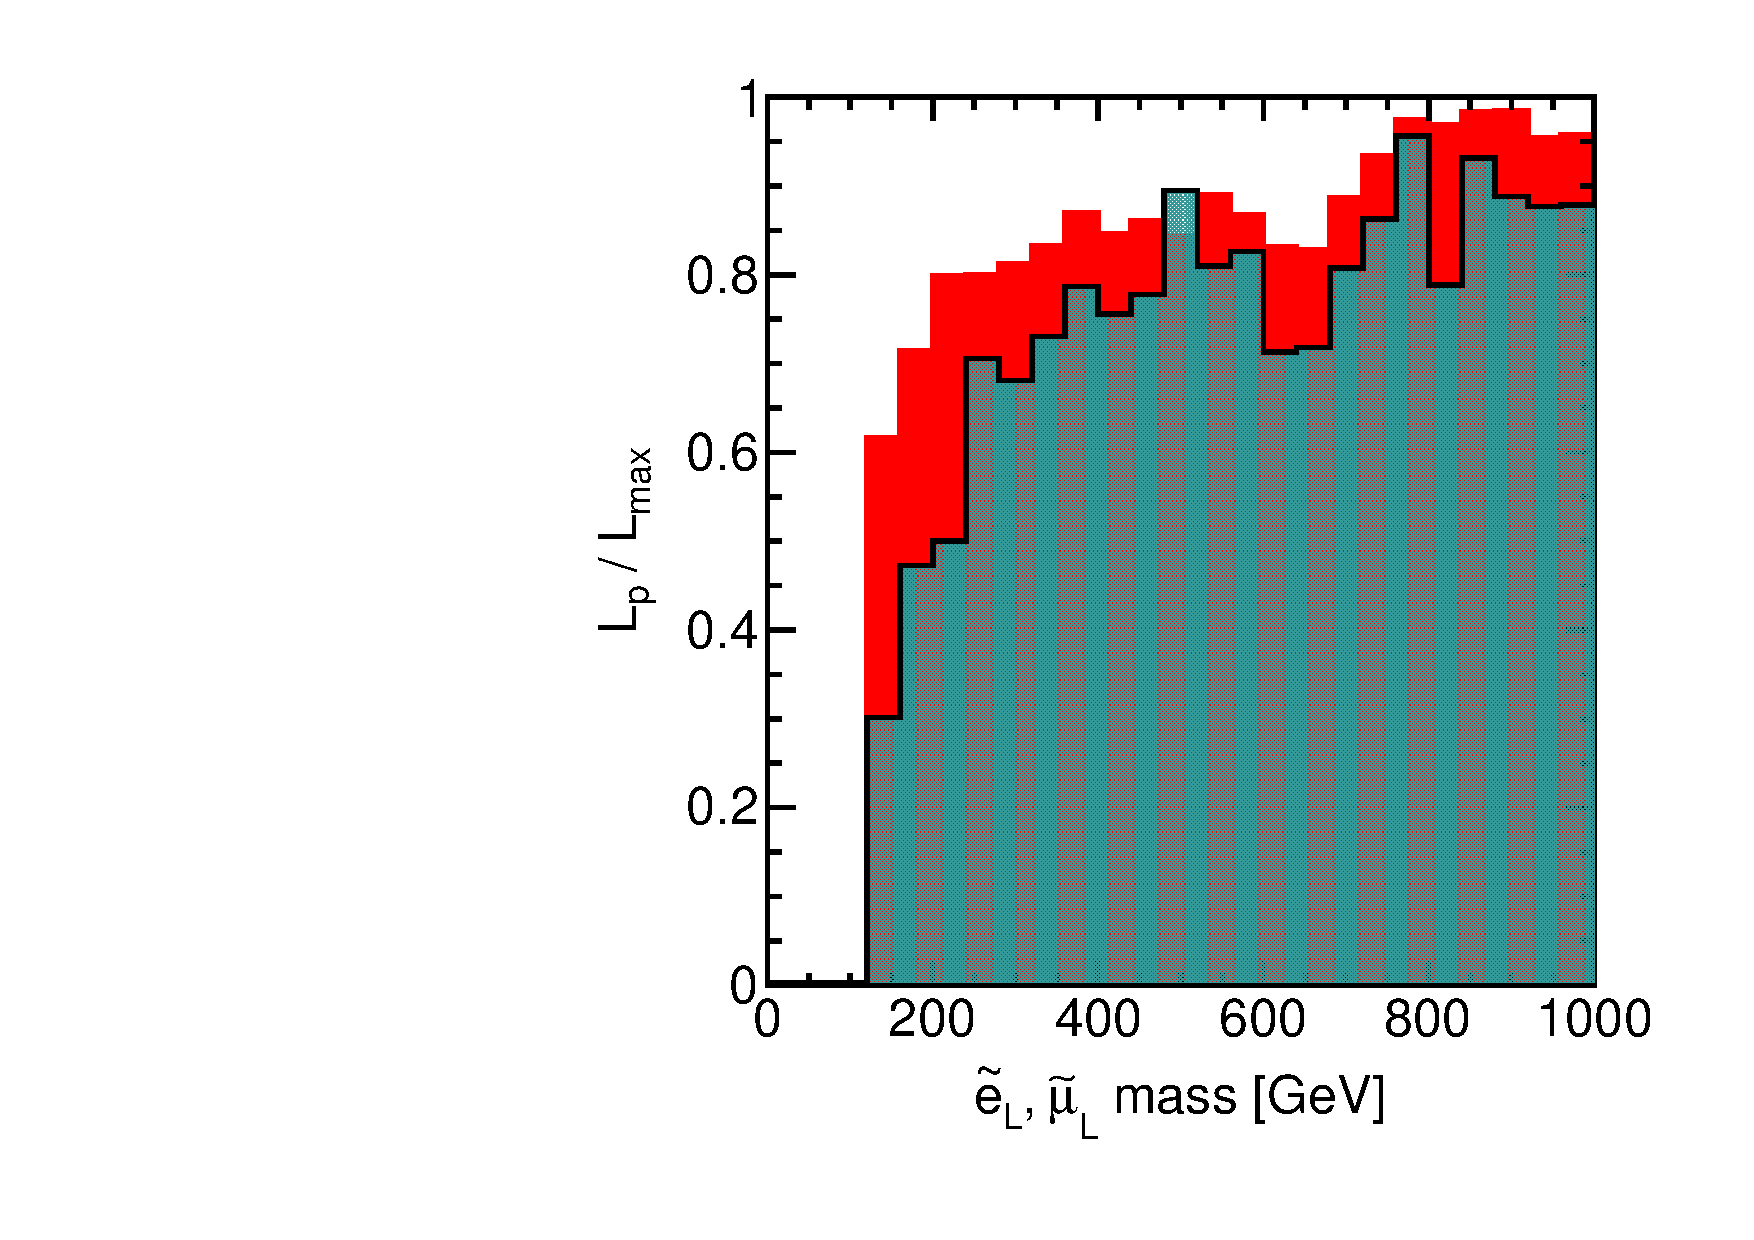
\includegraphics[height=5.5cm]{figs/fig_e_L.pdf} 
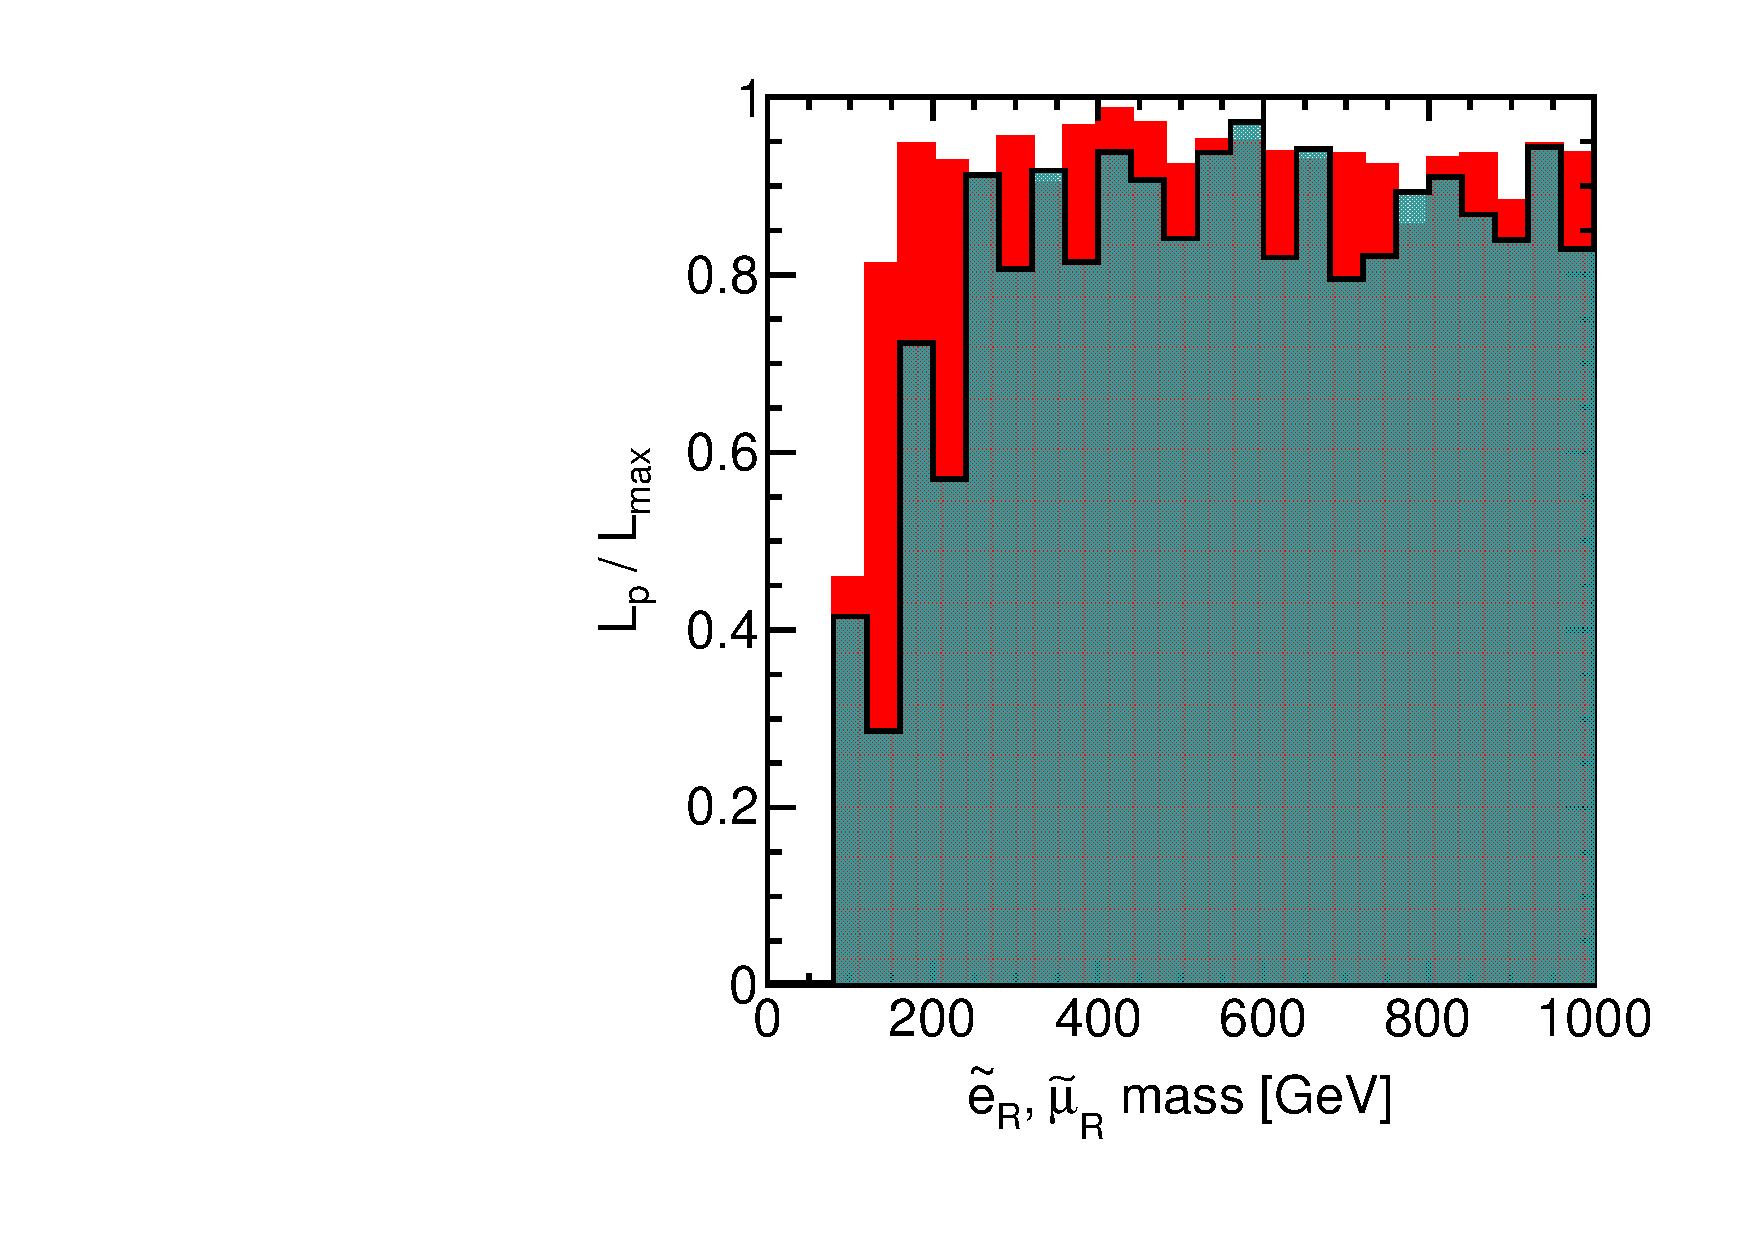
\includegraphics[height=5.5cm]{figs/fig_e_R.pdf} \\
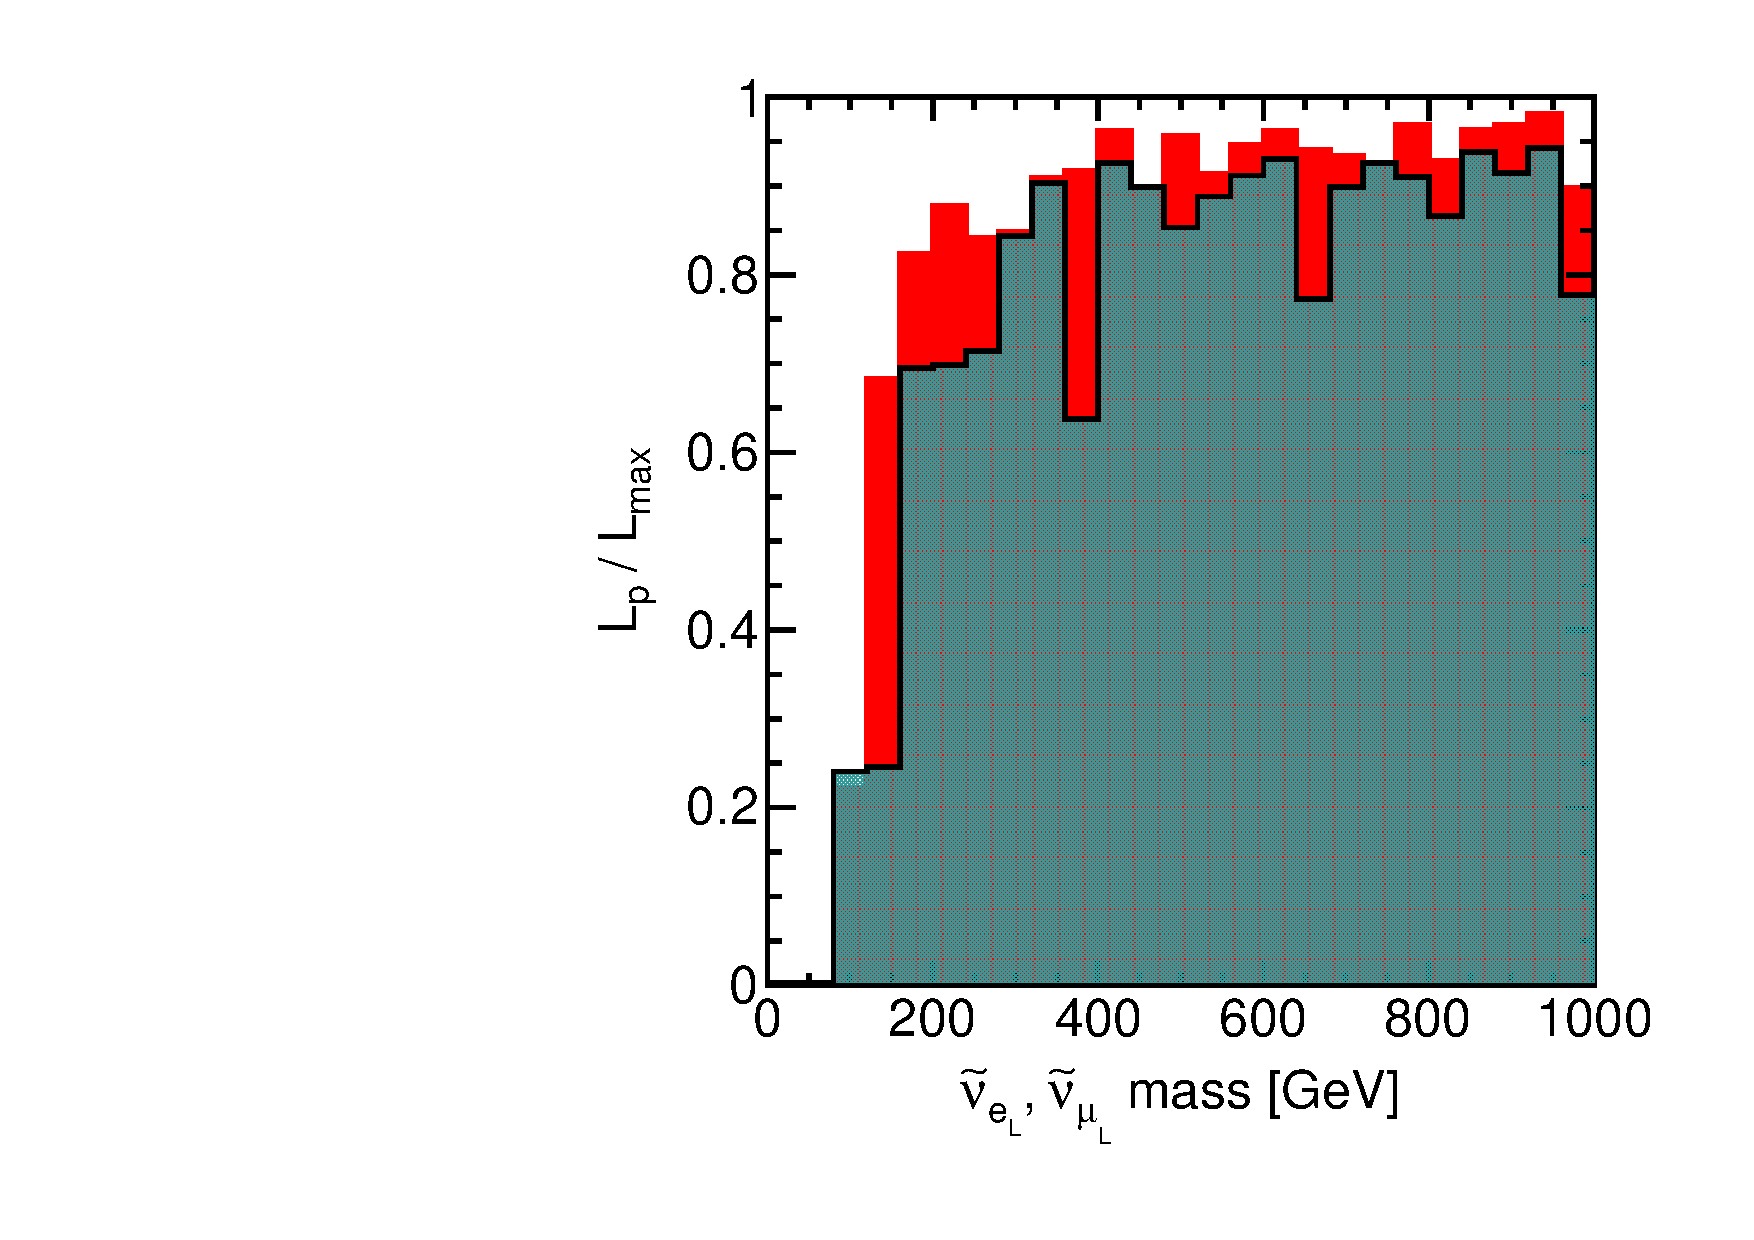
\includegraphics[height=5.5cm]{figs/fig_nu_e_L.pdf} 
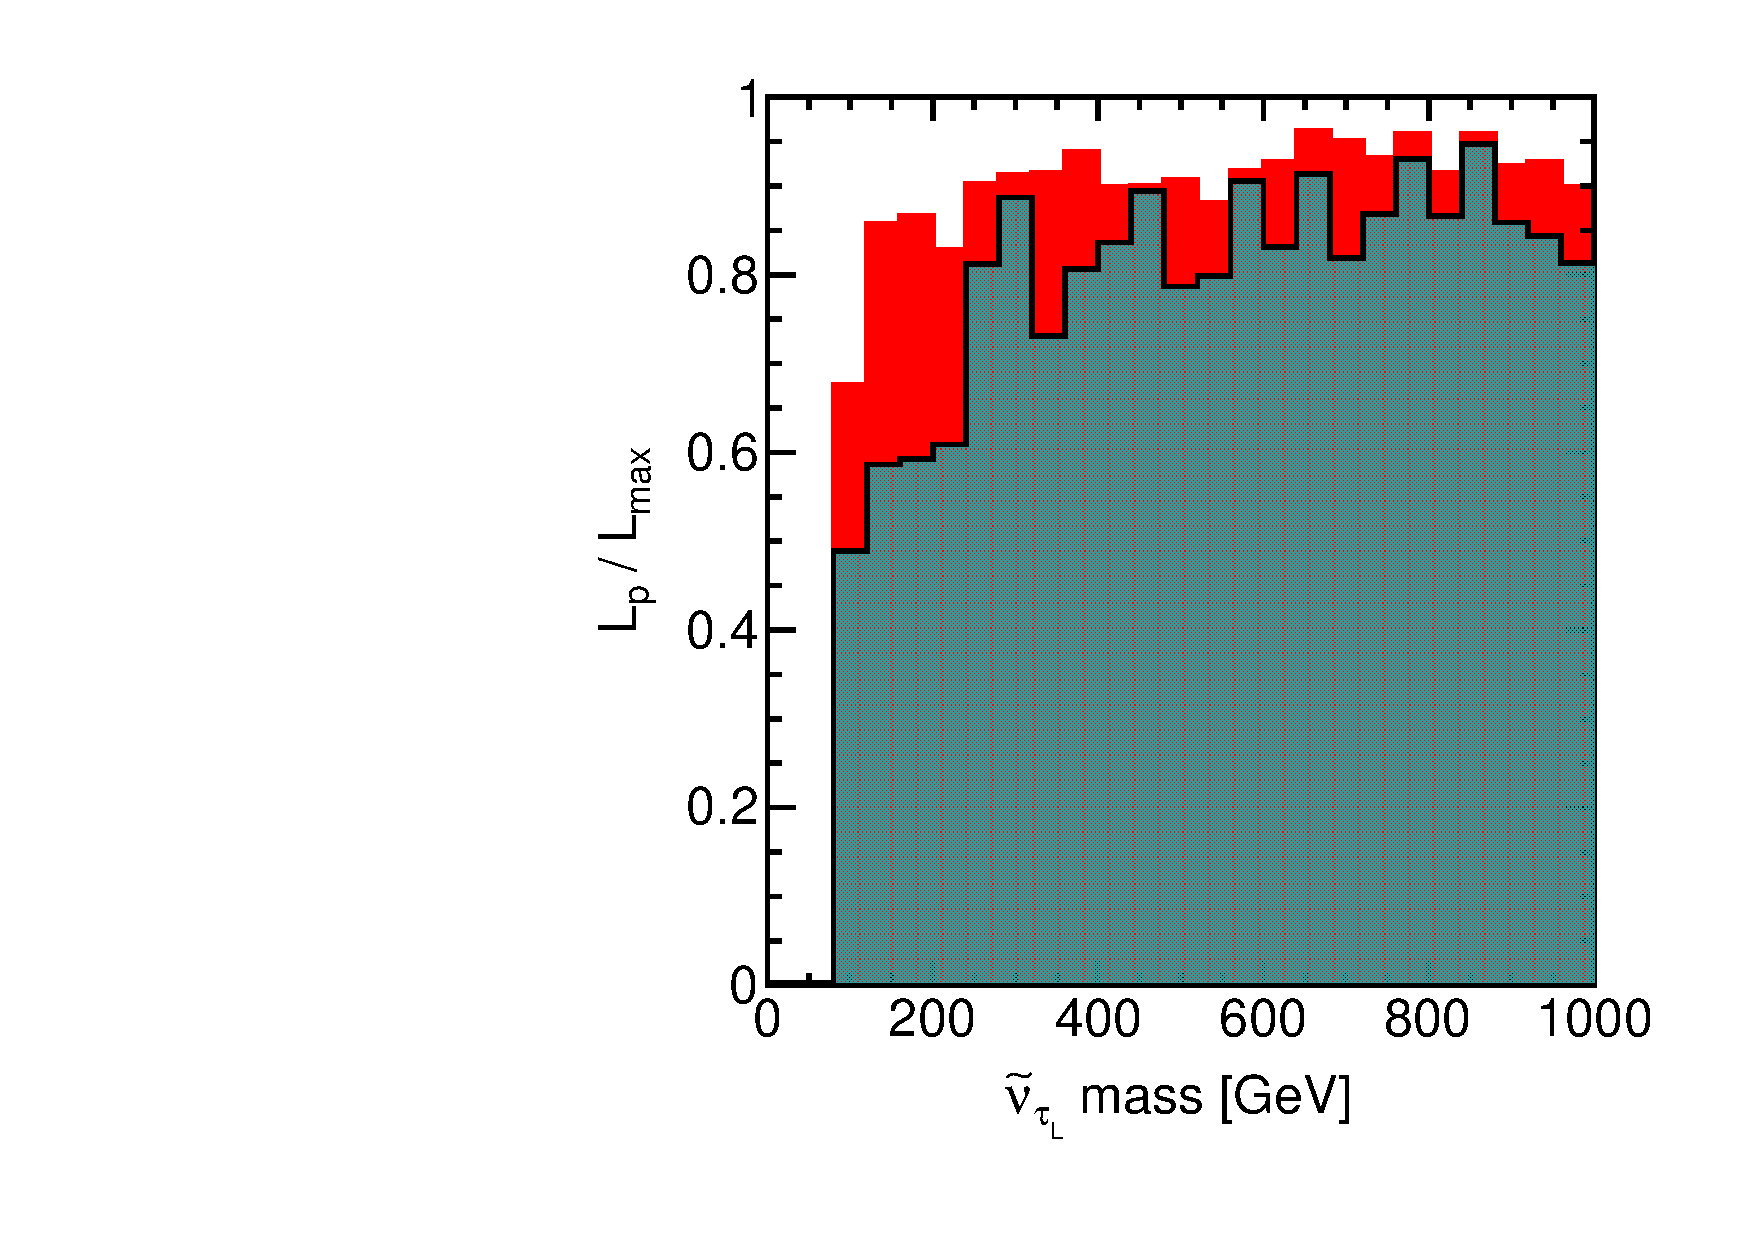
\includegraphics[height=5.5cm]{figs/fig_nu_tau_L.pdf} \\
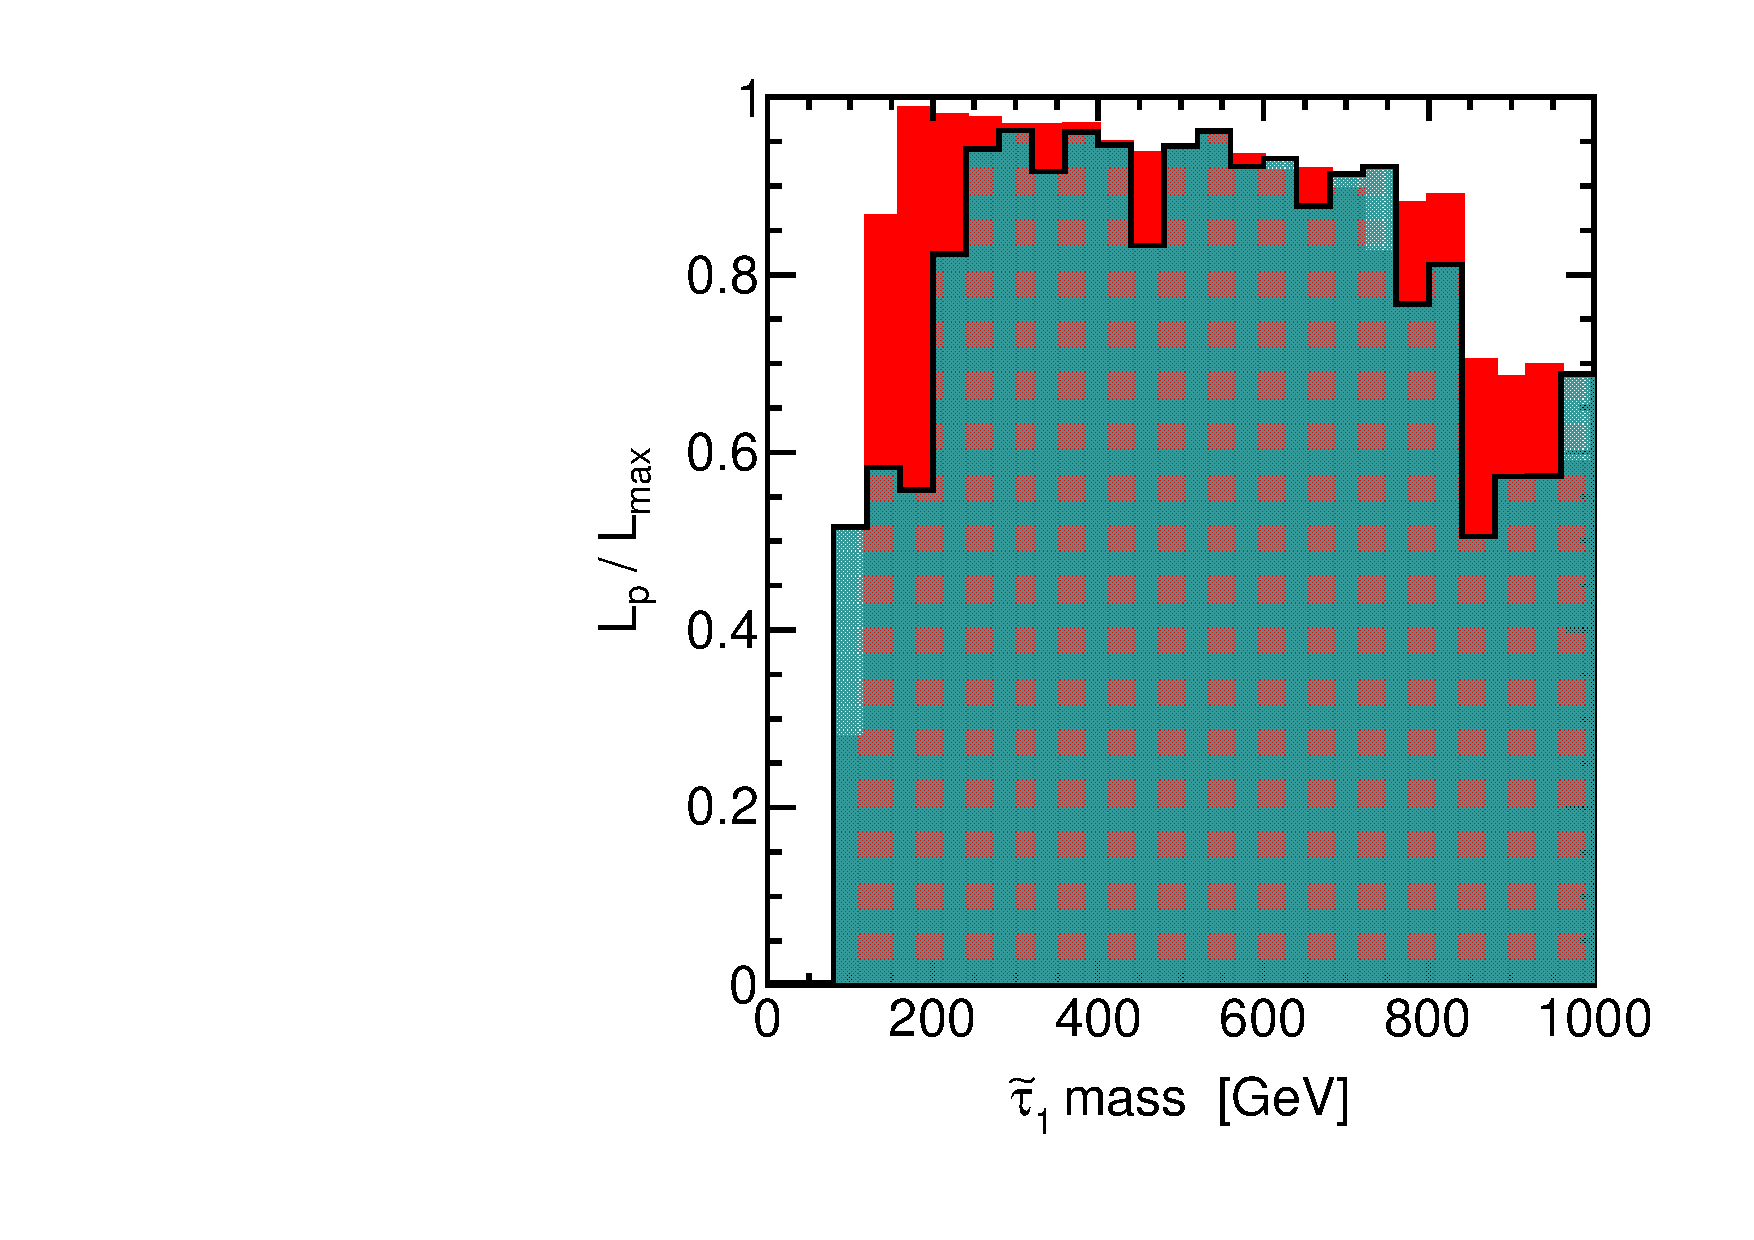
\includegraphics[height=5.5cm]{figs/fig_tau_1.pdf} 
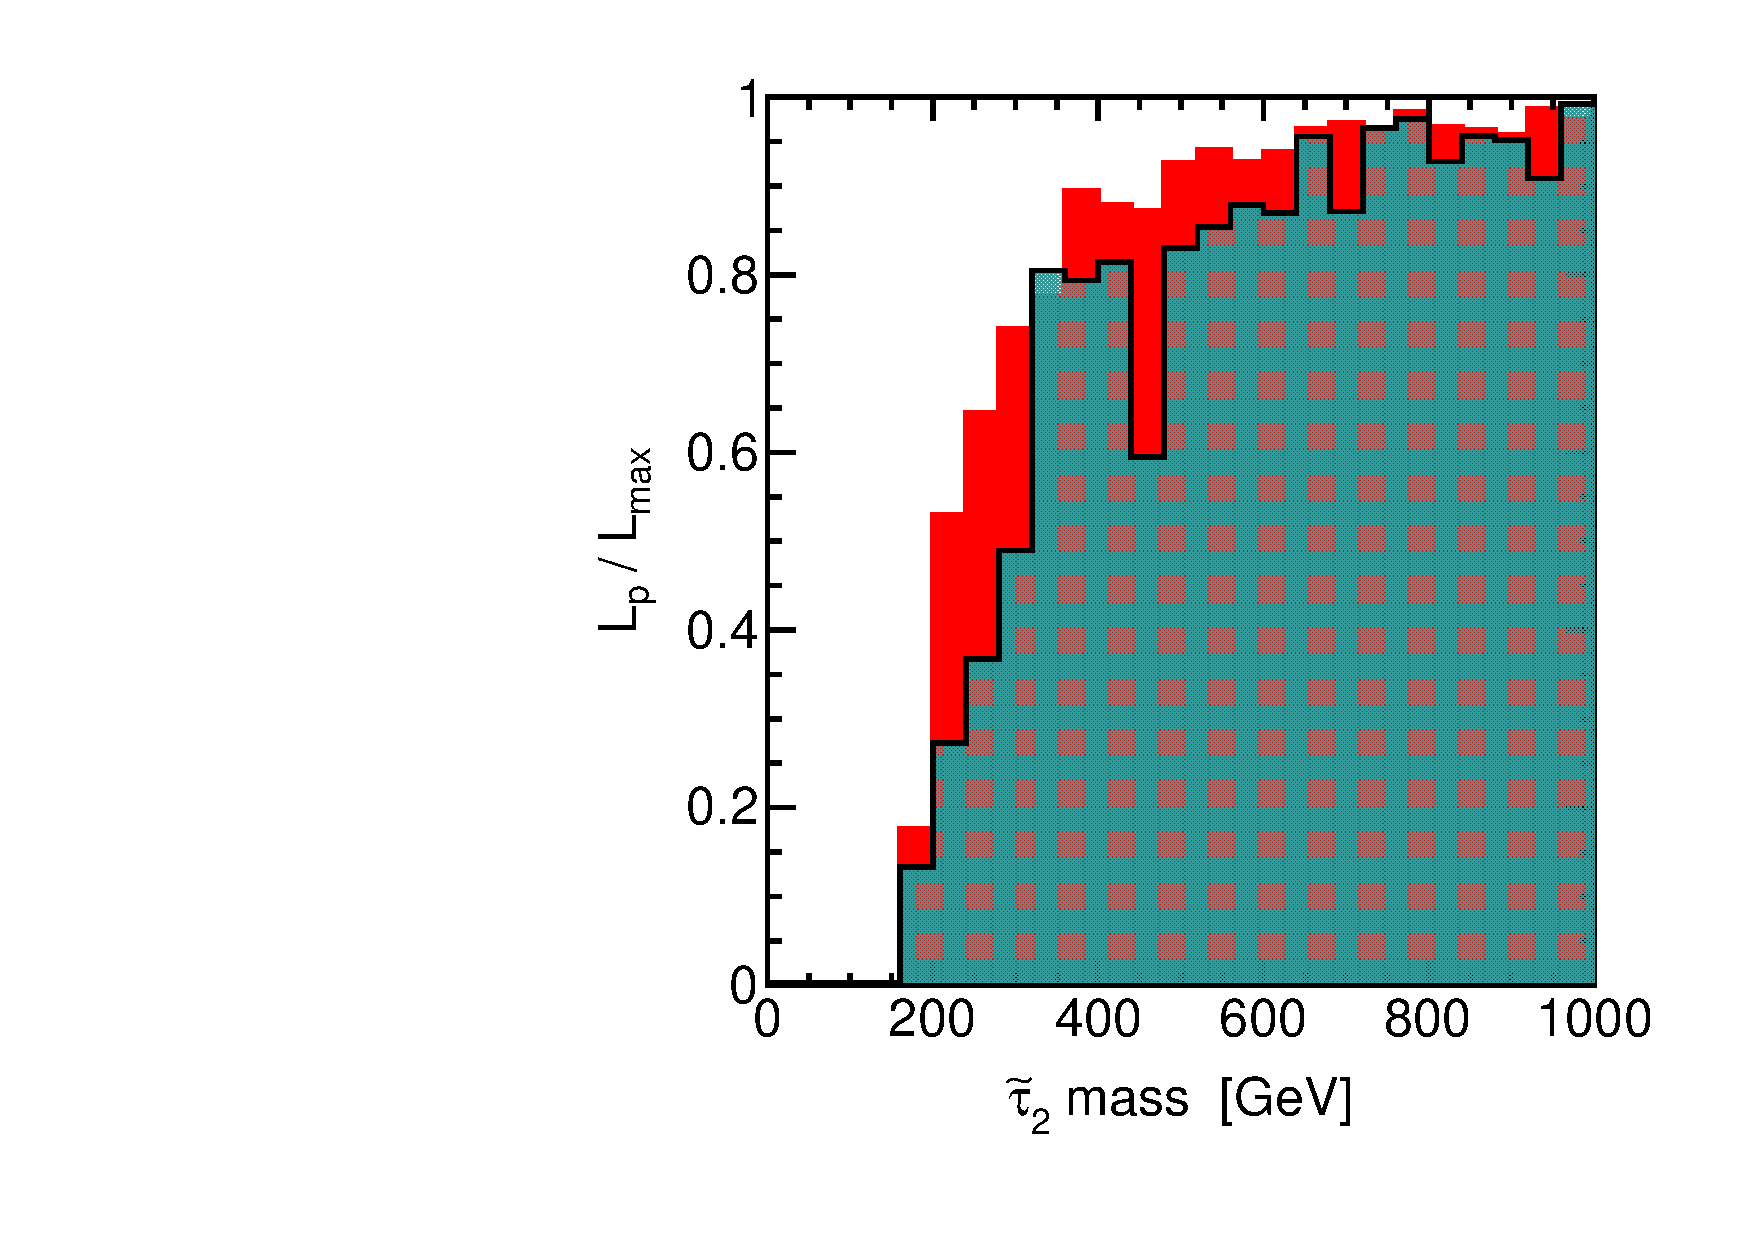
\includegraphics[height=5.5cm]{figs/fig_tau_2.pdf}
\caption{Ratios of profile likelihood $L_p$ to maximum likelihood $L_{max}$ shown for predictions for slepton masses.  The colored and shaded histograms show the distributions before and after the inclusion of the CMS results.}
\label{fig:LRwcms:sl}
\end{center}
\end{figure}

\begin{figure}[htbp]
\begin{center}
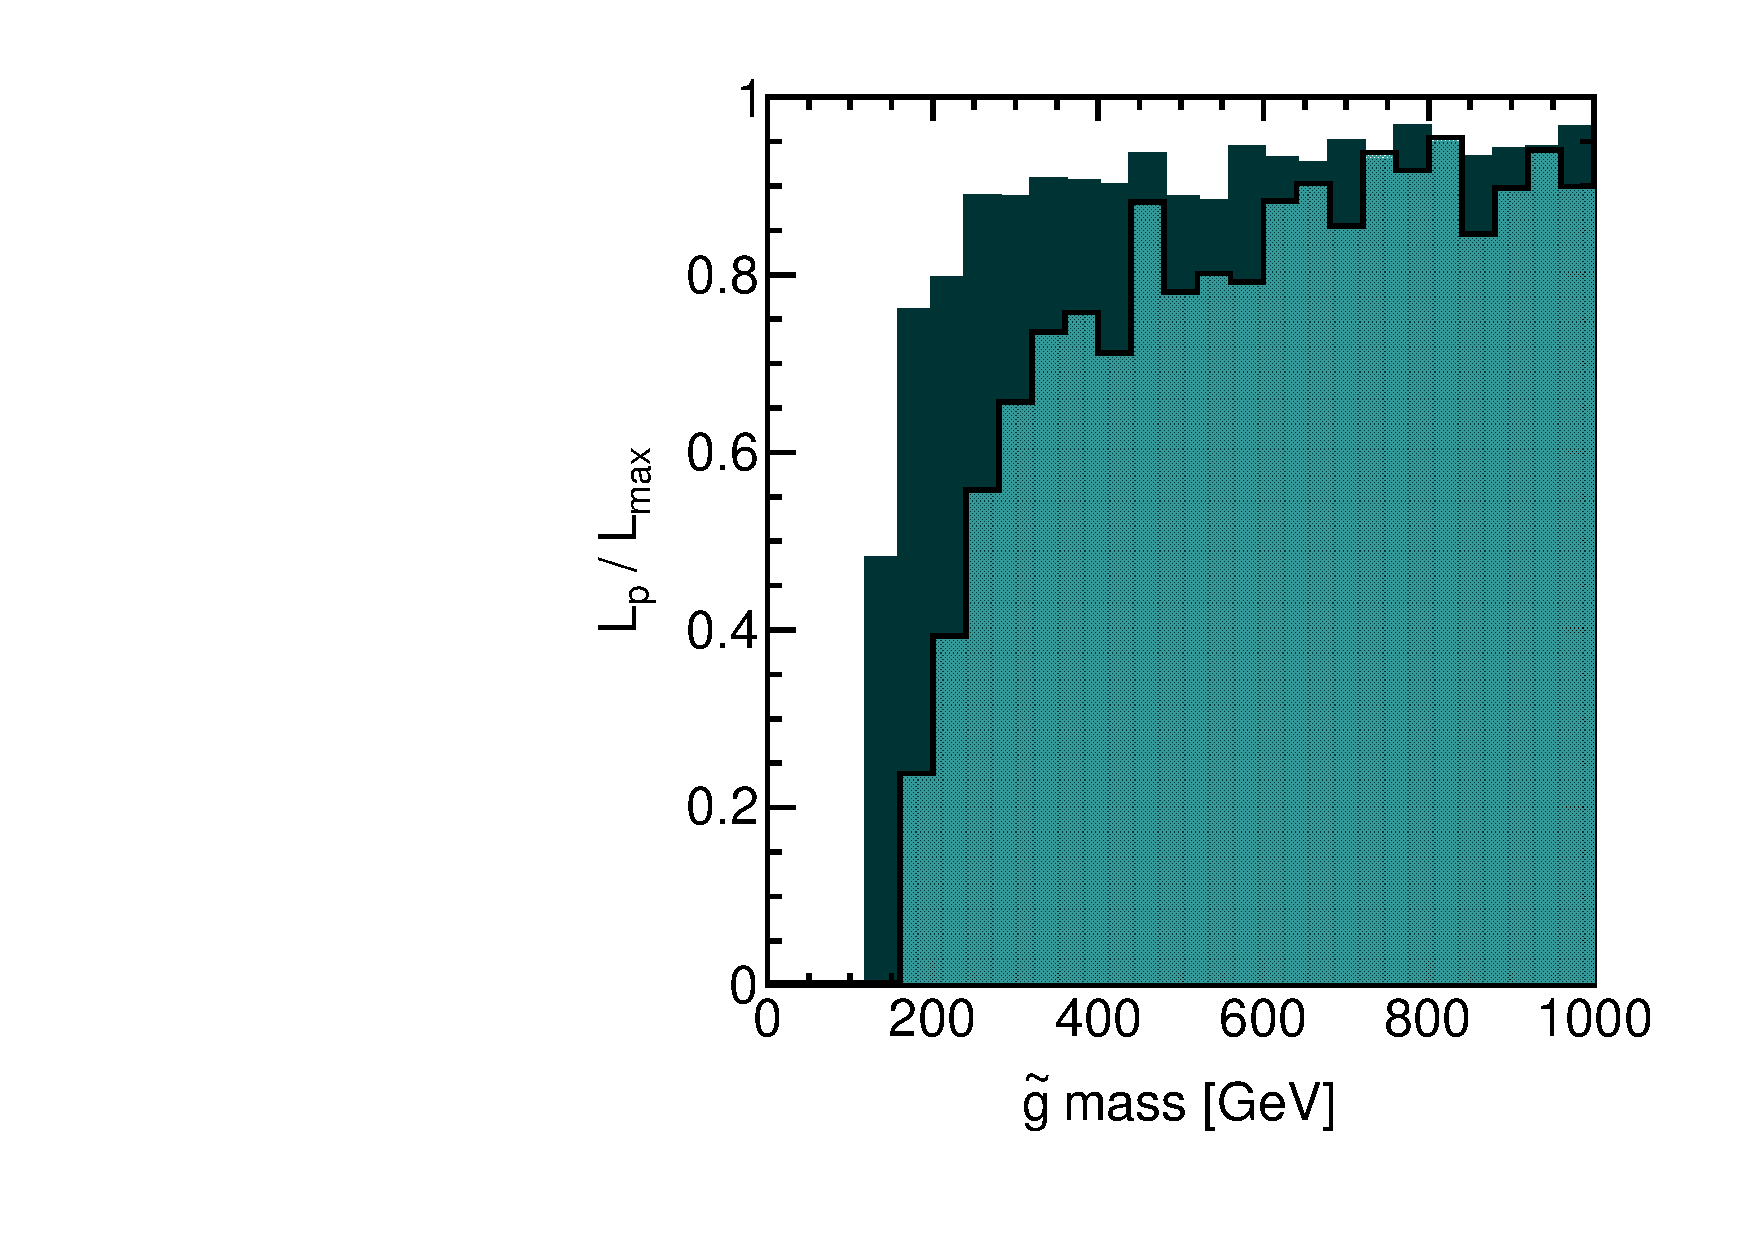
\includegraphics[height=5.5cm]{figs/fig_g.pdf} 
\caption{Ratios of profile likelihood $L_p$ to maximum likelihood $L_{max}$ shown for the gluino mass.  The colored and shaded histograms show the distributions before and after the inclusion of the CMS results.}
\label{fig:LRwcms:g}
\end{center}
\end{figure}


\begin{figure}[htbp]
\begin{center}
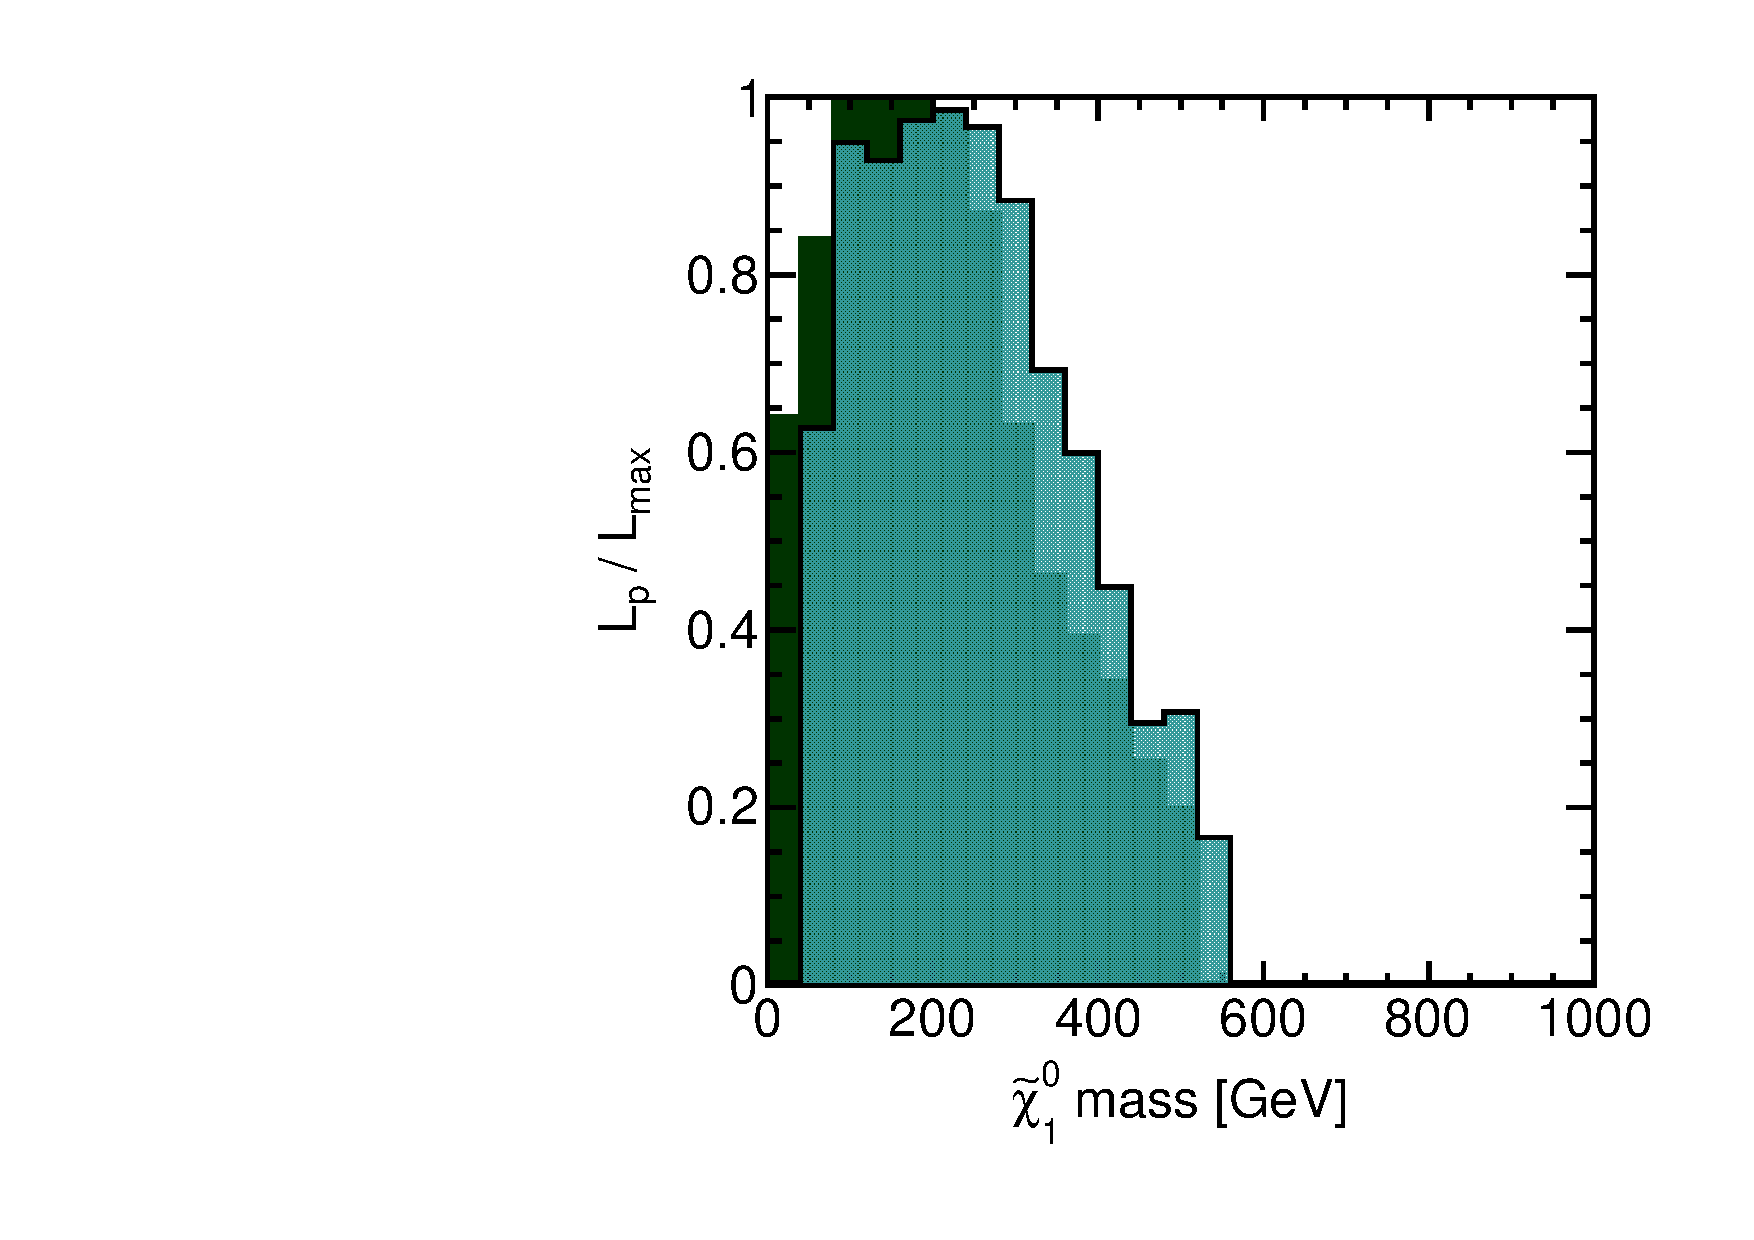
\includegraphics[height=5.5cm]{figs/fig_chi_1_0.pdf} 
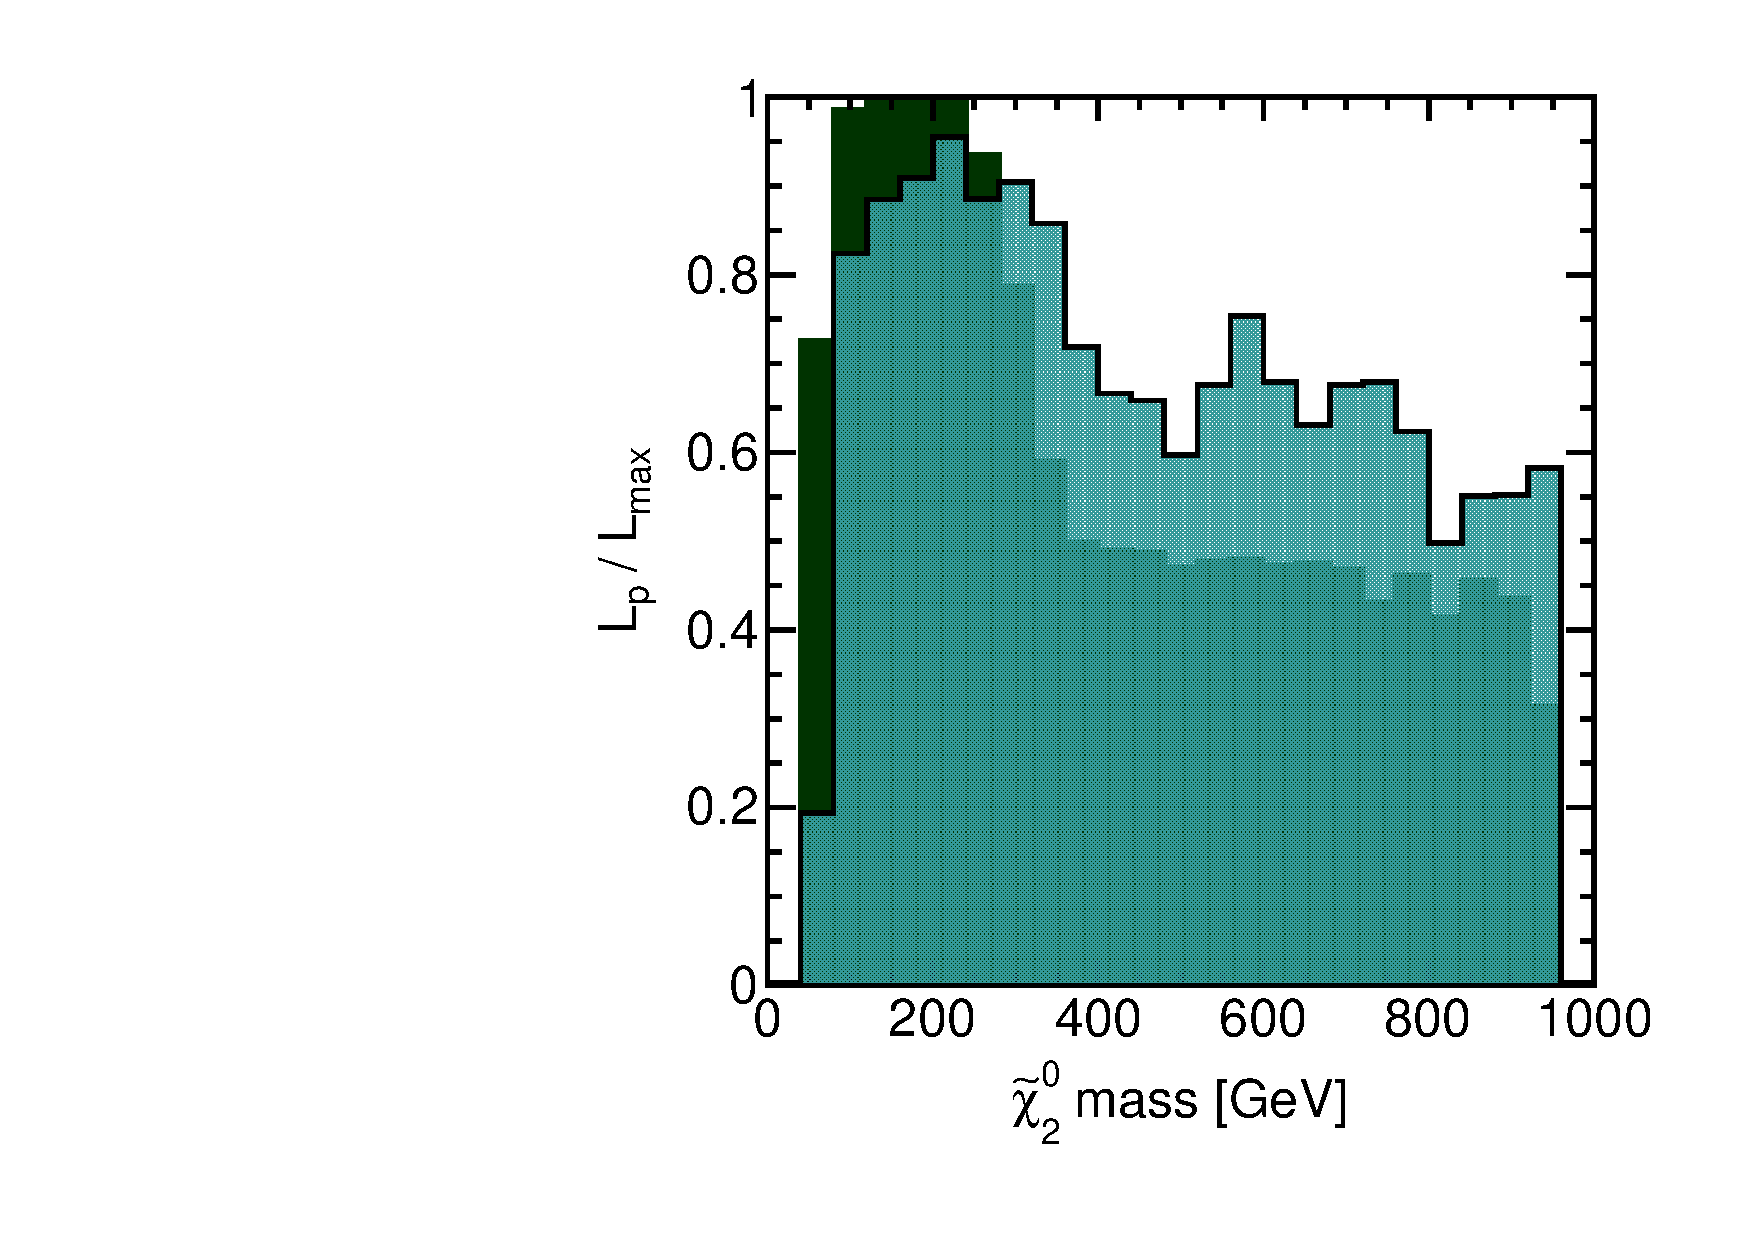
\includegraphics[height=5.5cm]{figs/fig_chi_2_0.pdf} \\
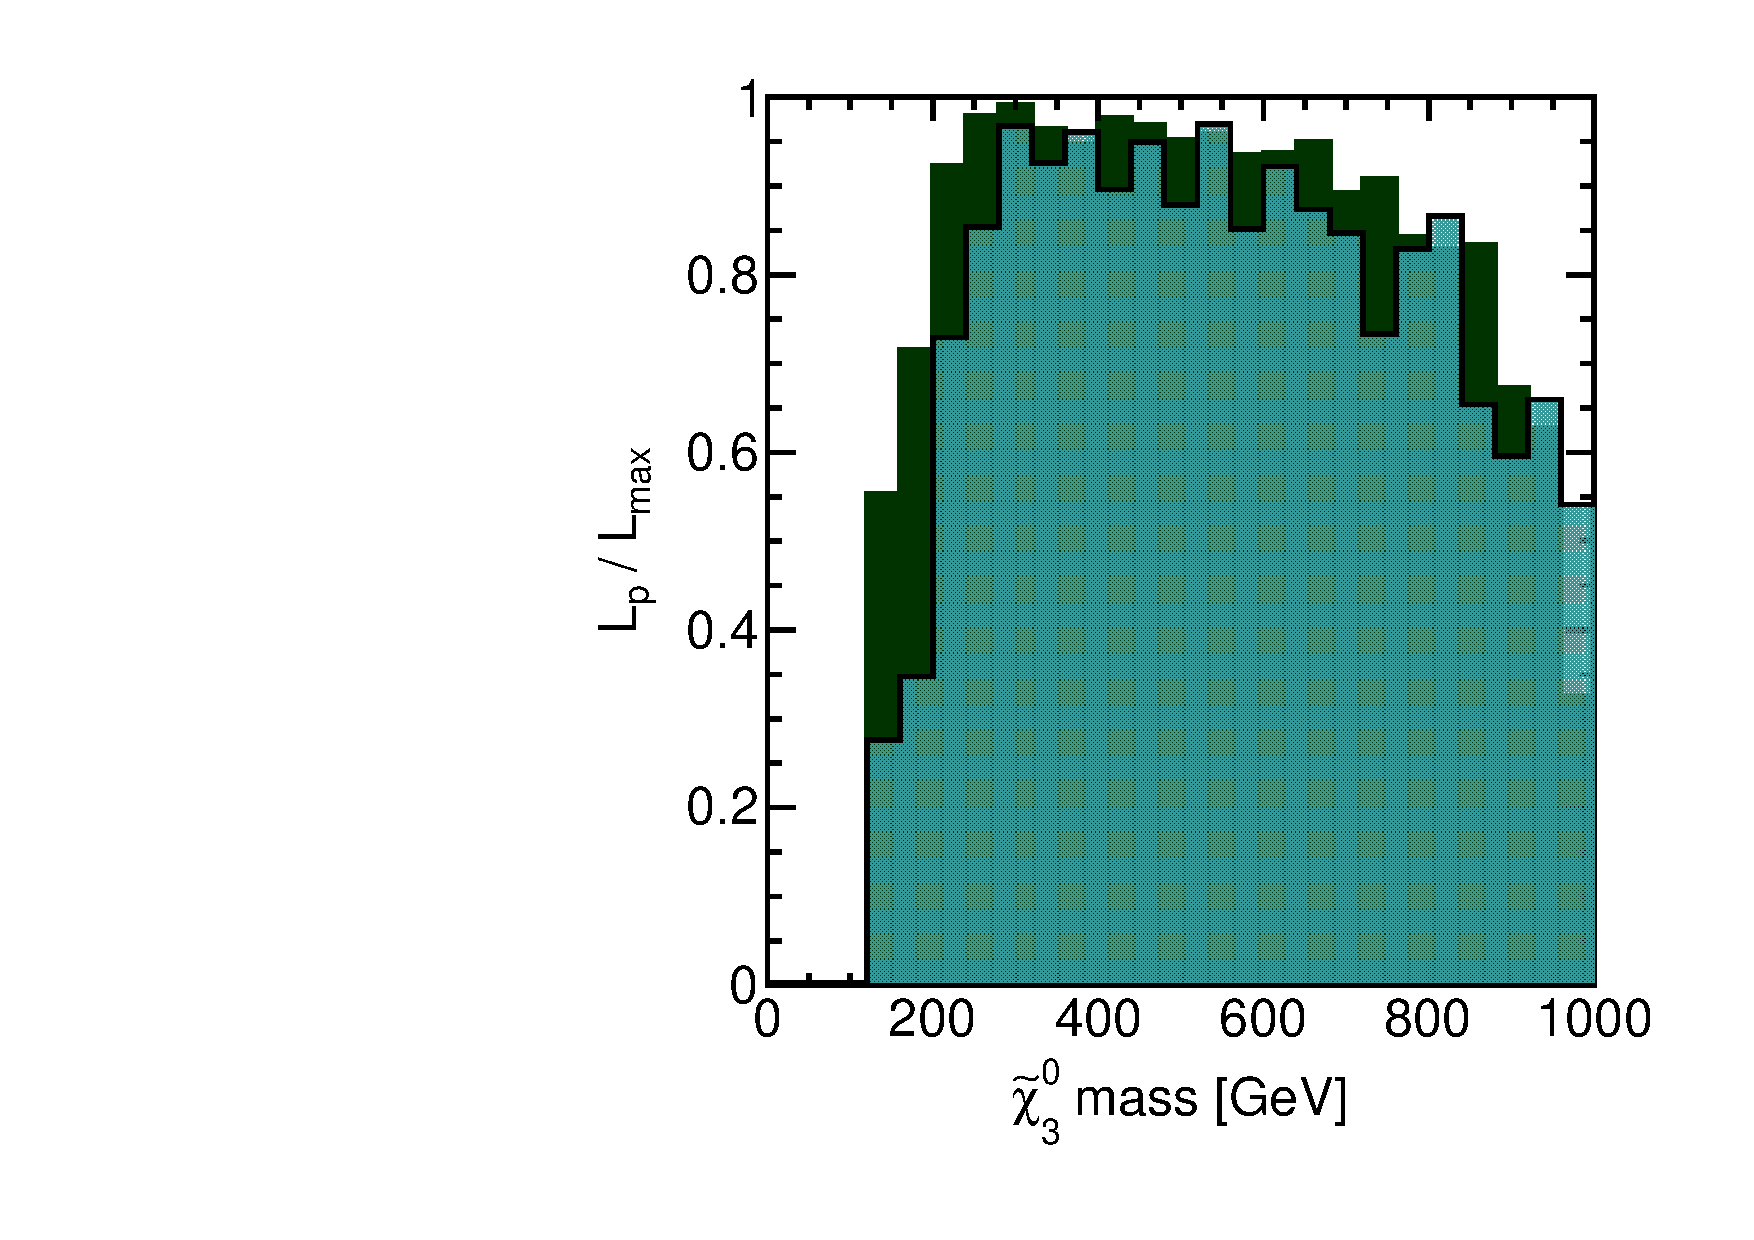
\includegraphics[height=5.5cm]{figs/fig_chi_3_0.pdf} 
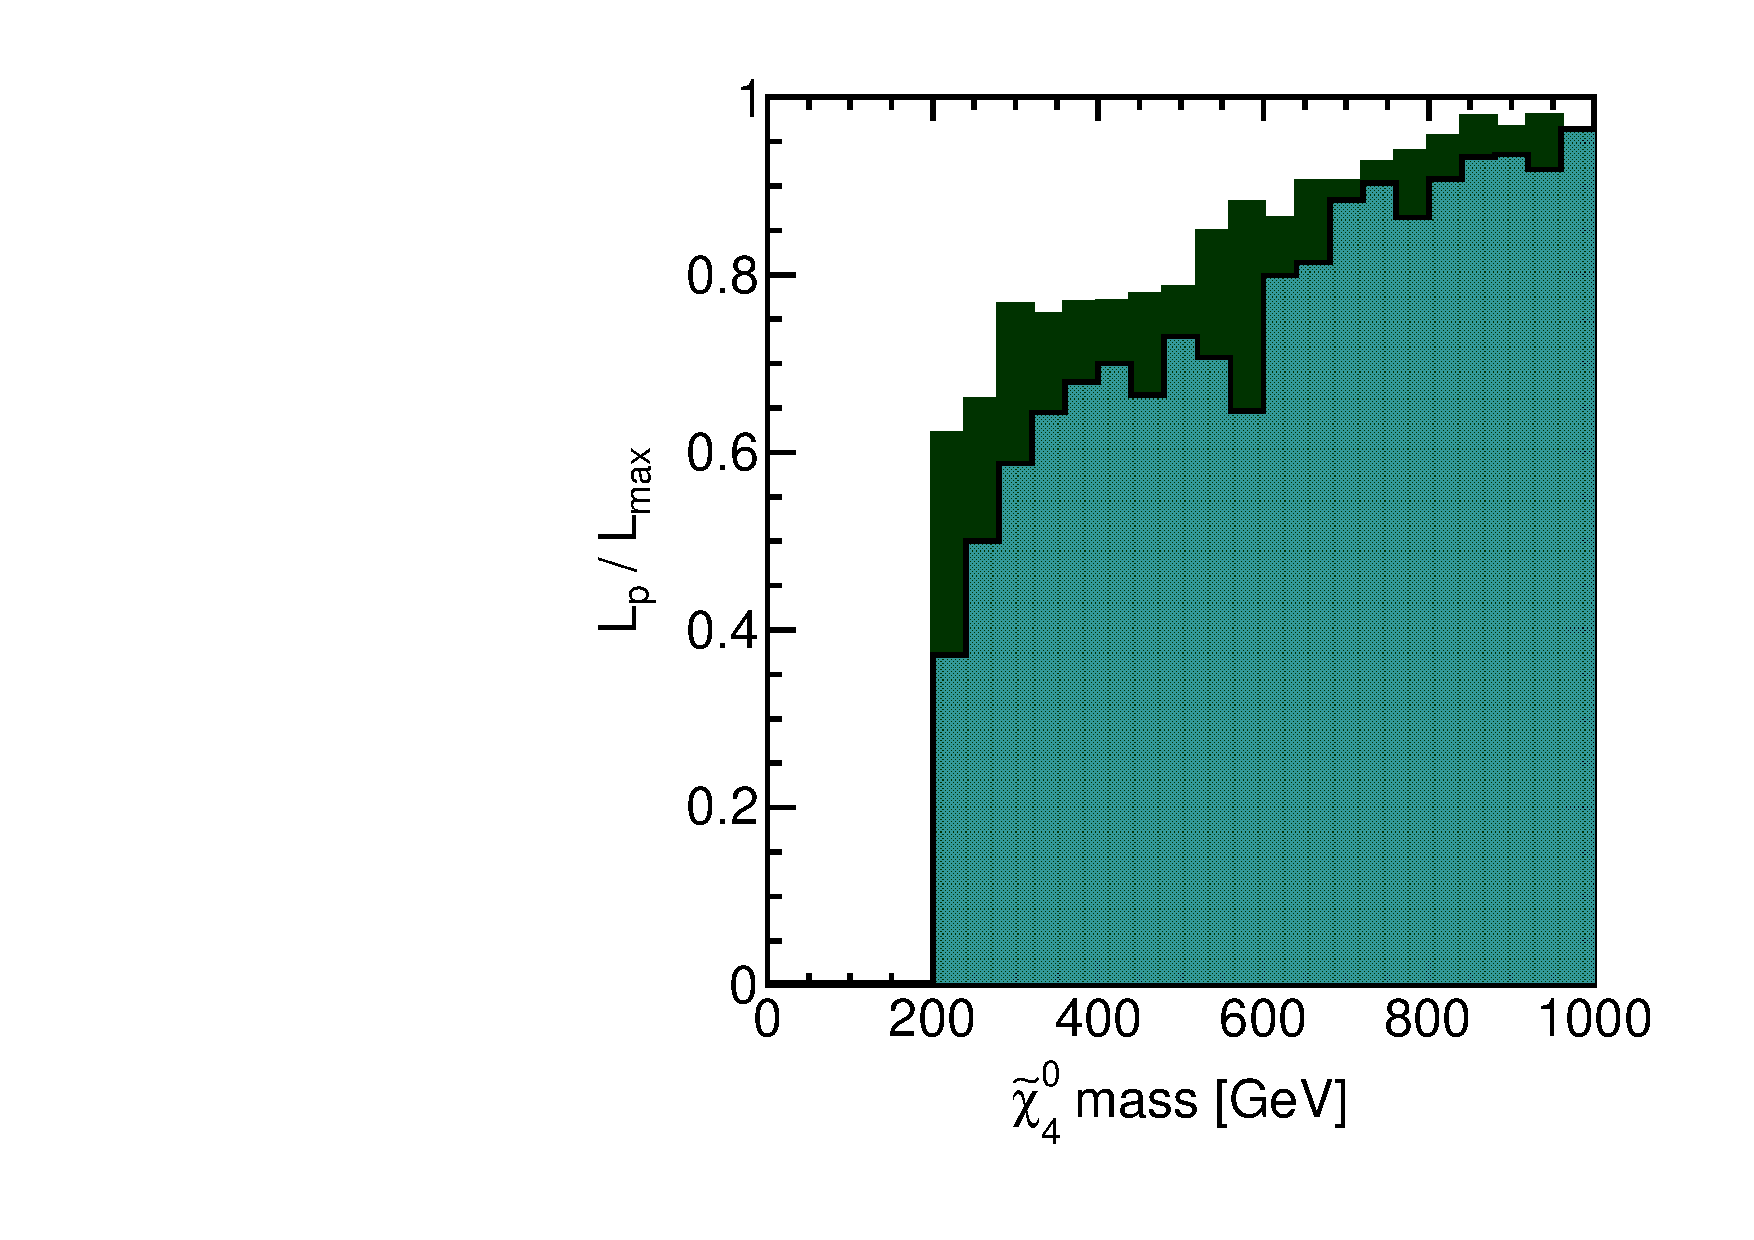
\includegraphics[height=5.5cm]{figs/fig_chi_4_0.pdf} 
\caption{Ratios of profile likelihood $L_p$ to maximum likelihood $L_{max}$ shown for the neutralino masses.  The colored and shaded histograms show the distributions before and after the inclusion of the CMS results.}
\label{fig:LRwcms_chi0}
\end{center}
\end{figure}

\begin{figure}[htbp]
\begin{center}
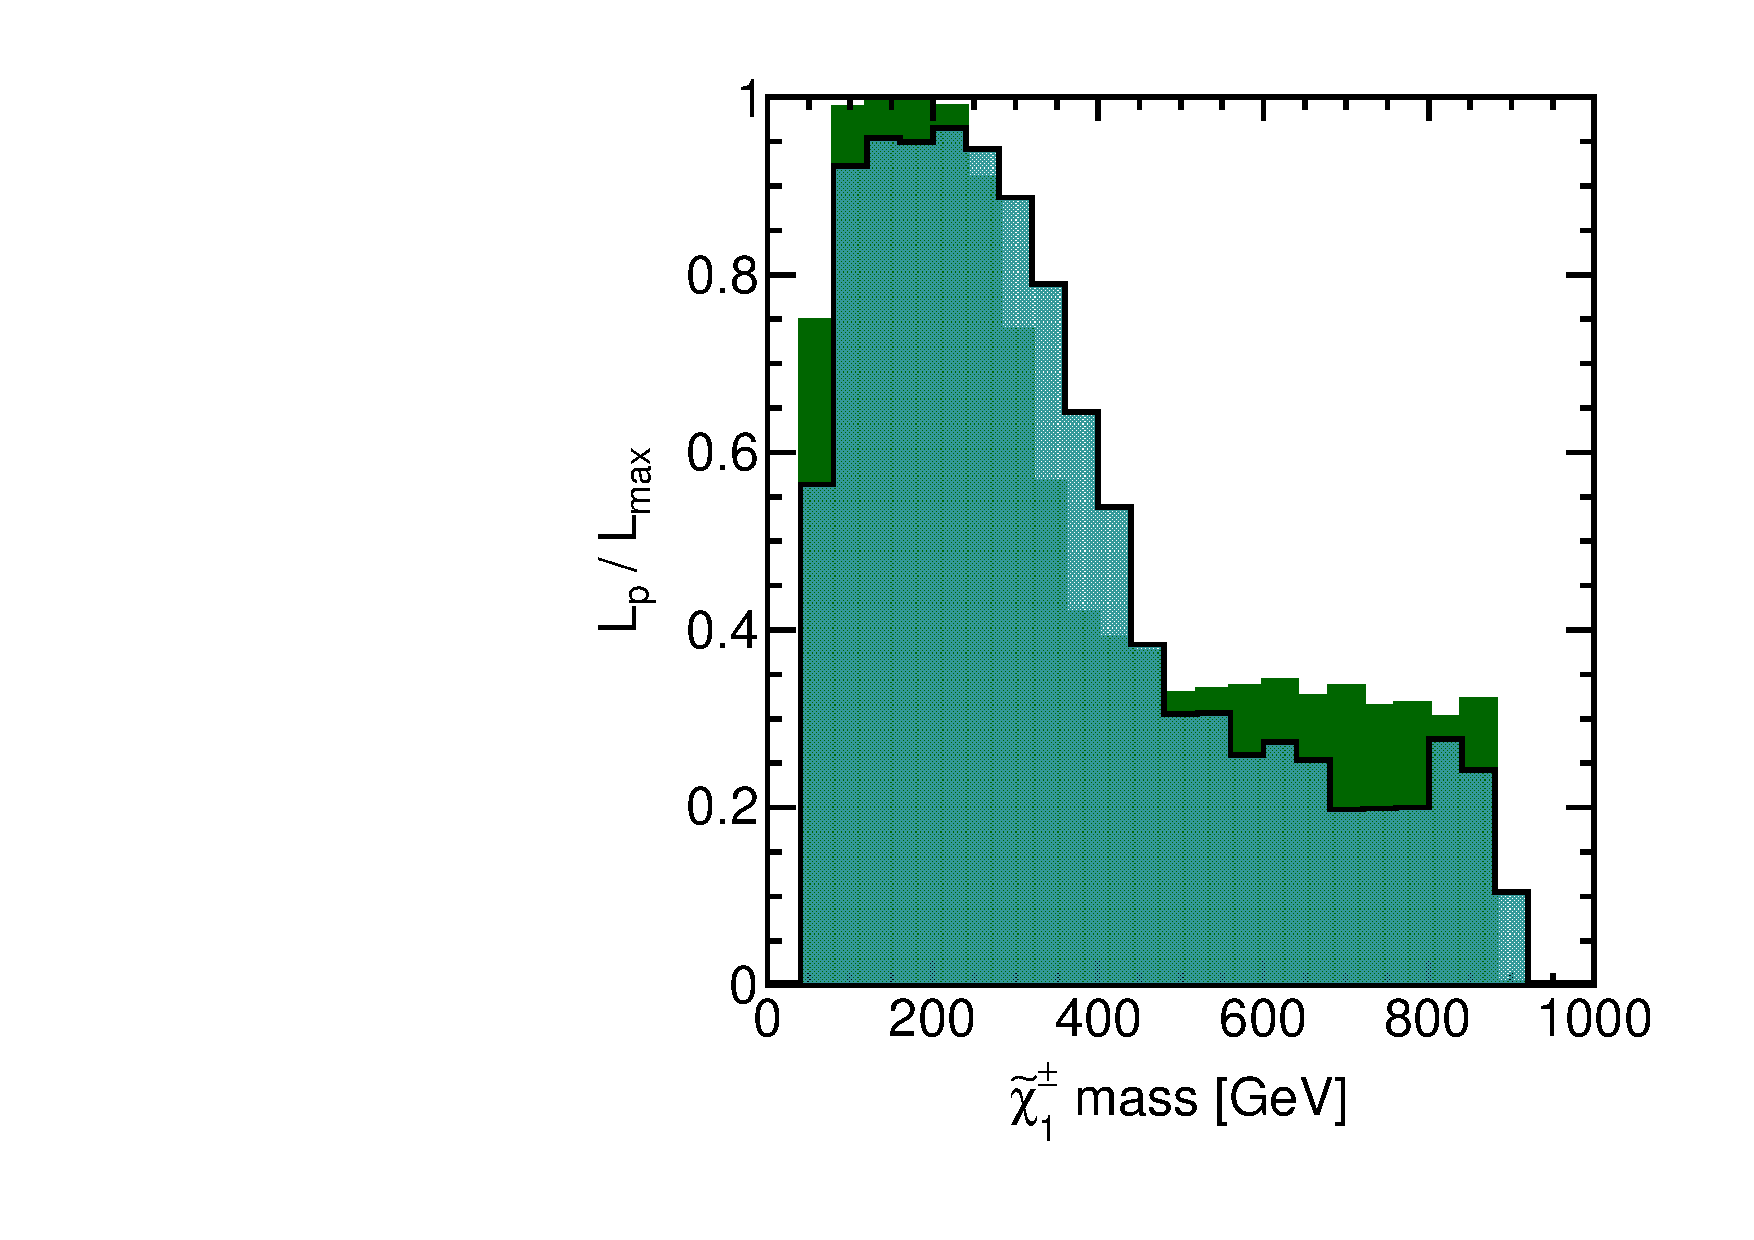
\includegraphics[height=5.5cm]{figs/fig_chi_1_pm.pdf} 
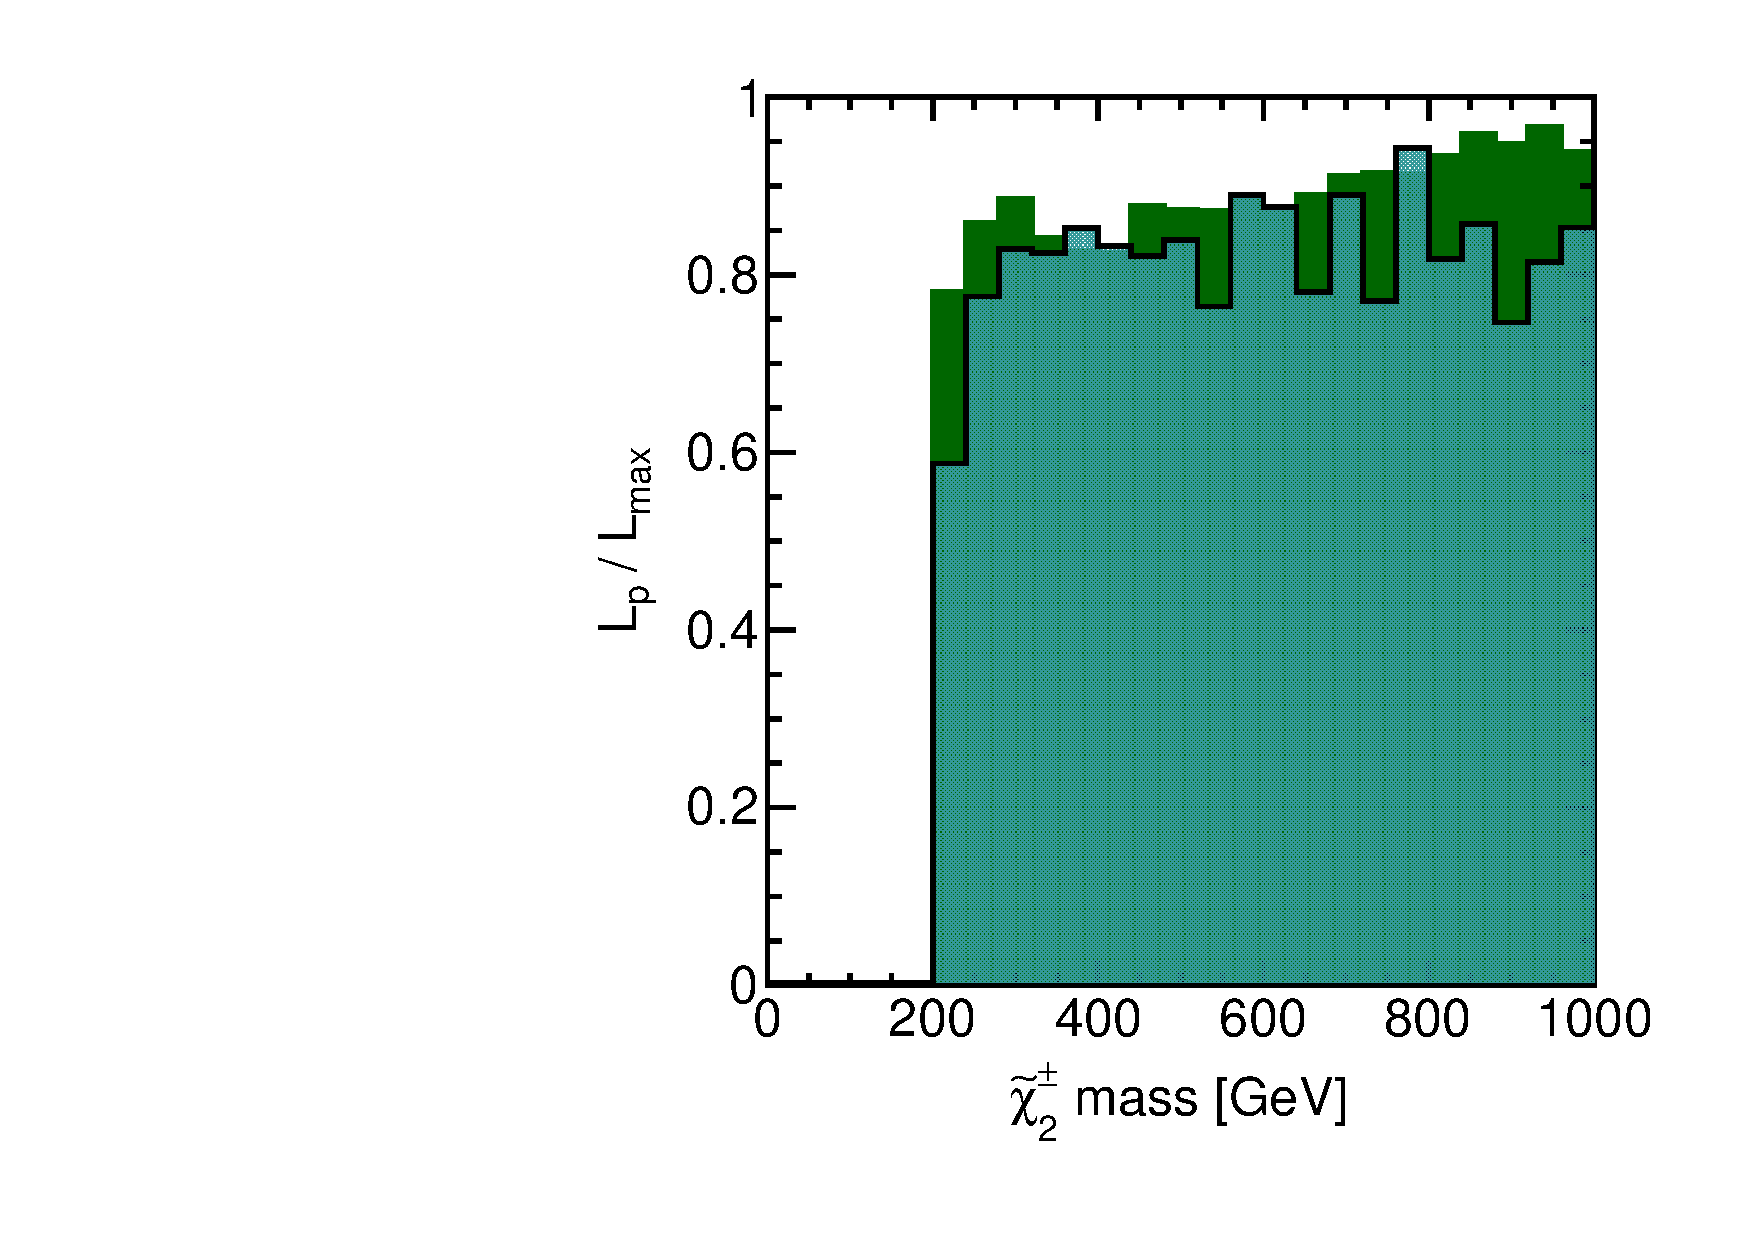
\includegraphics[height=5.5cm]{figs/fig_chi_2_pm.pdf}
\caption{Ratios of profile likelihood $L_p$ to maximum likelihood $L_{max}$ shown for chargino masses.  The colored and shaded histograms show the distributions before and after the inclusion of the CMS results.}
\label{fig:LRwcms_chipm}
\end{center}
\end{figure}


\begin{figure}[htbp]
\begin{center}
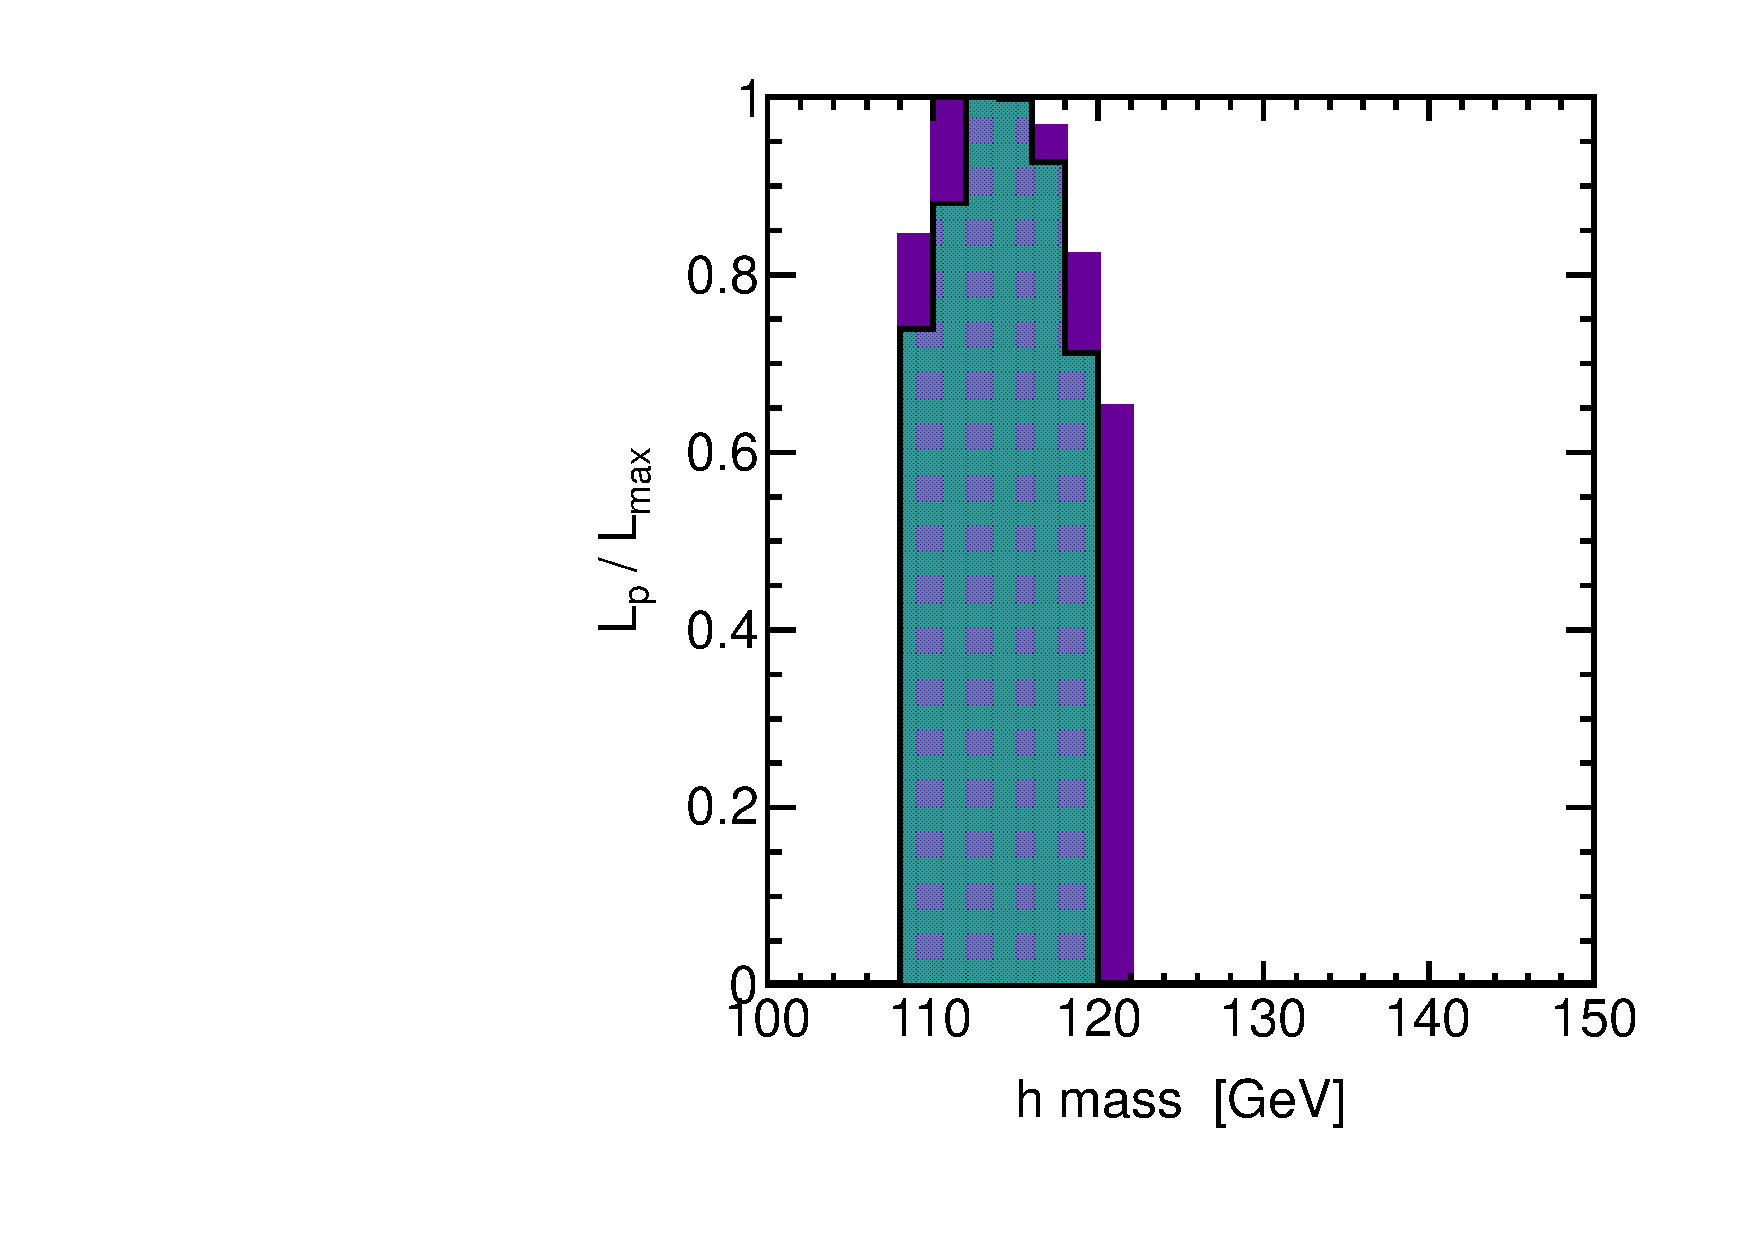
\includegraphics[height=5.5cm]{figs/fig_h.pdf} 
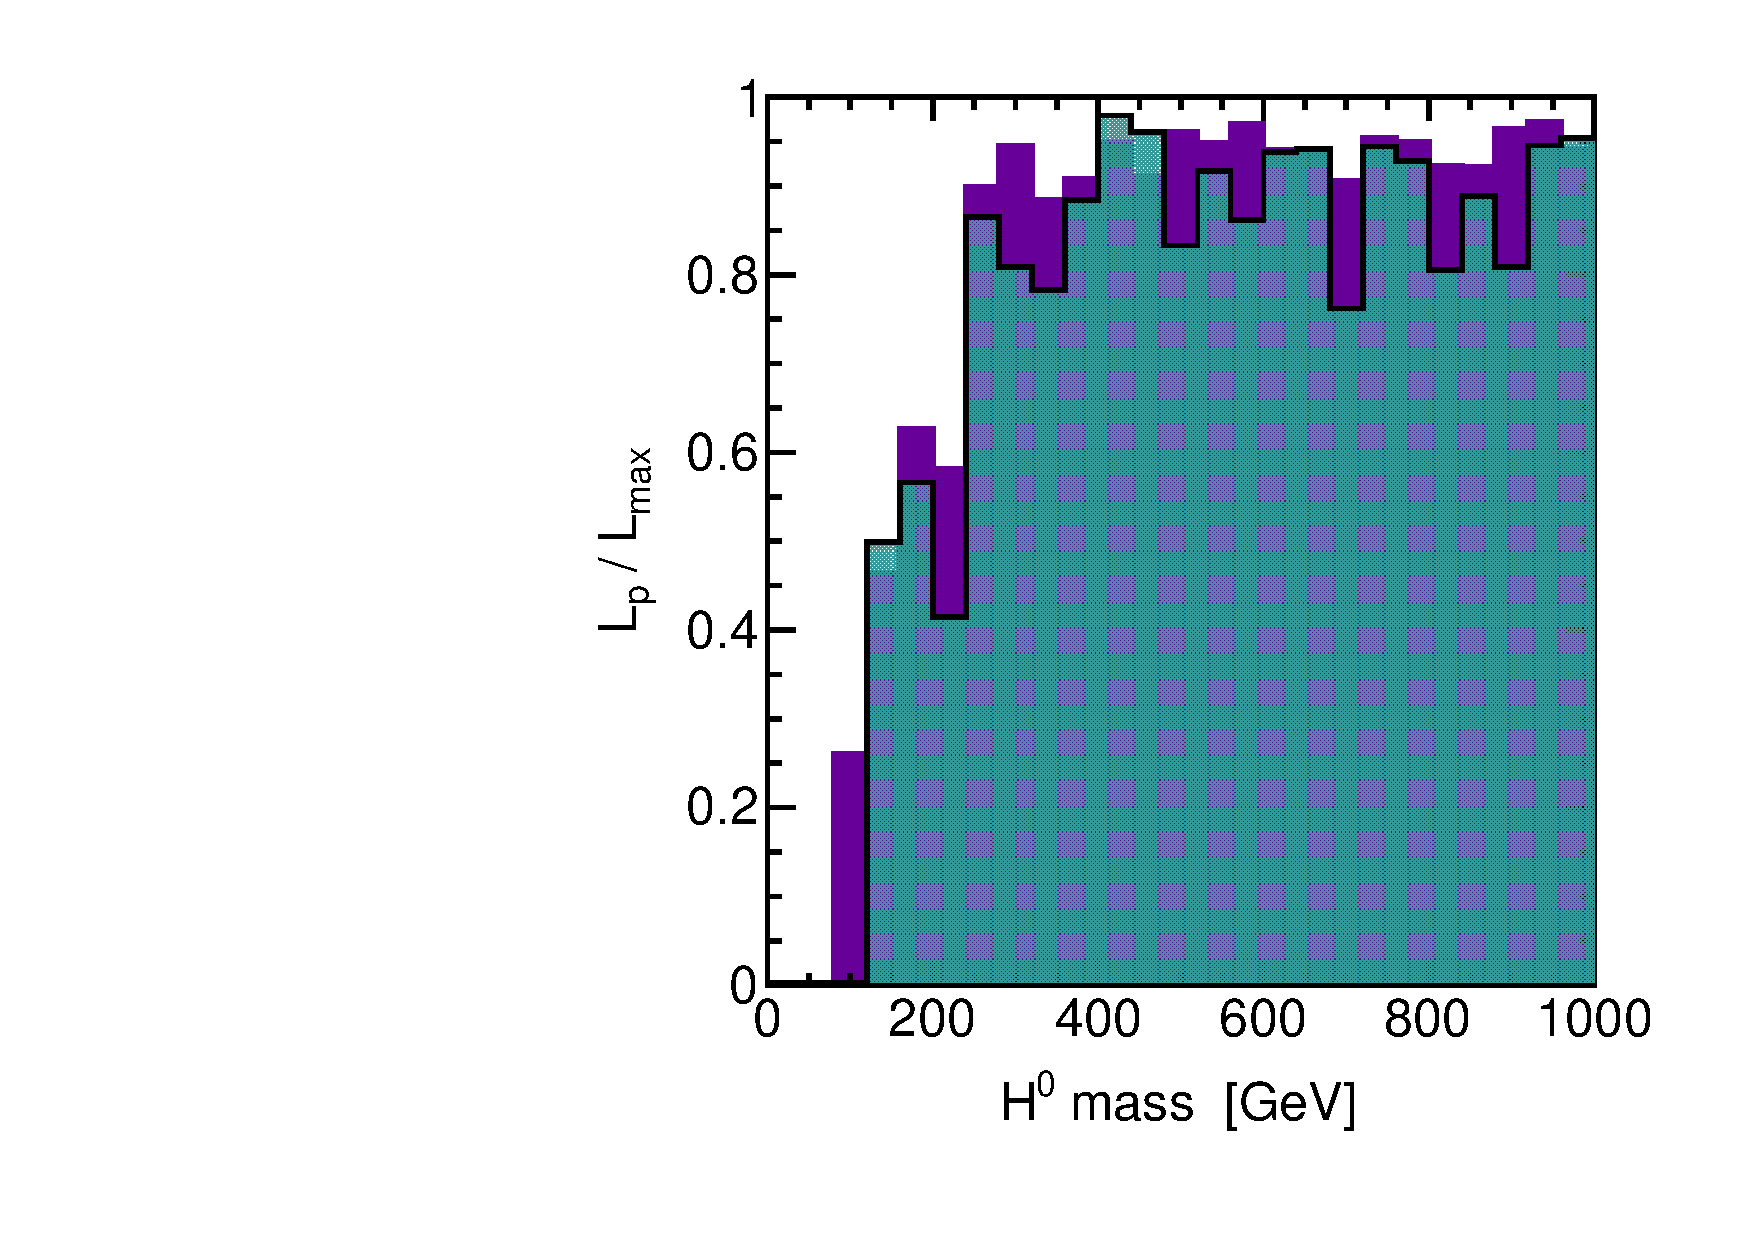
\includegraphics[height=5.5cm]{figs/fig_H0.pdf} \\
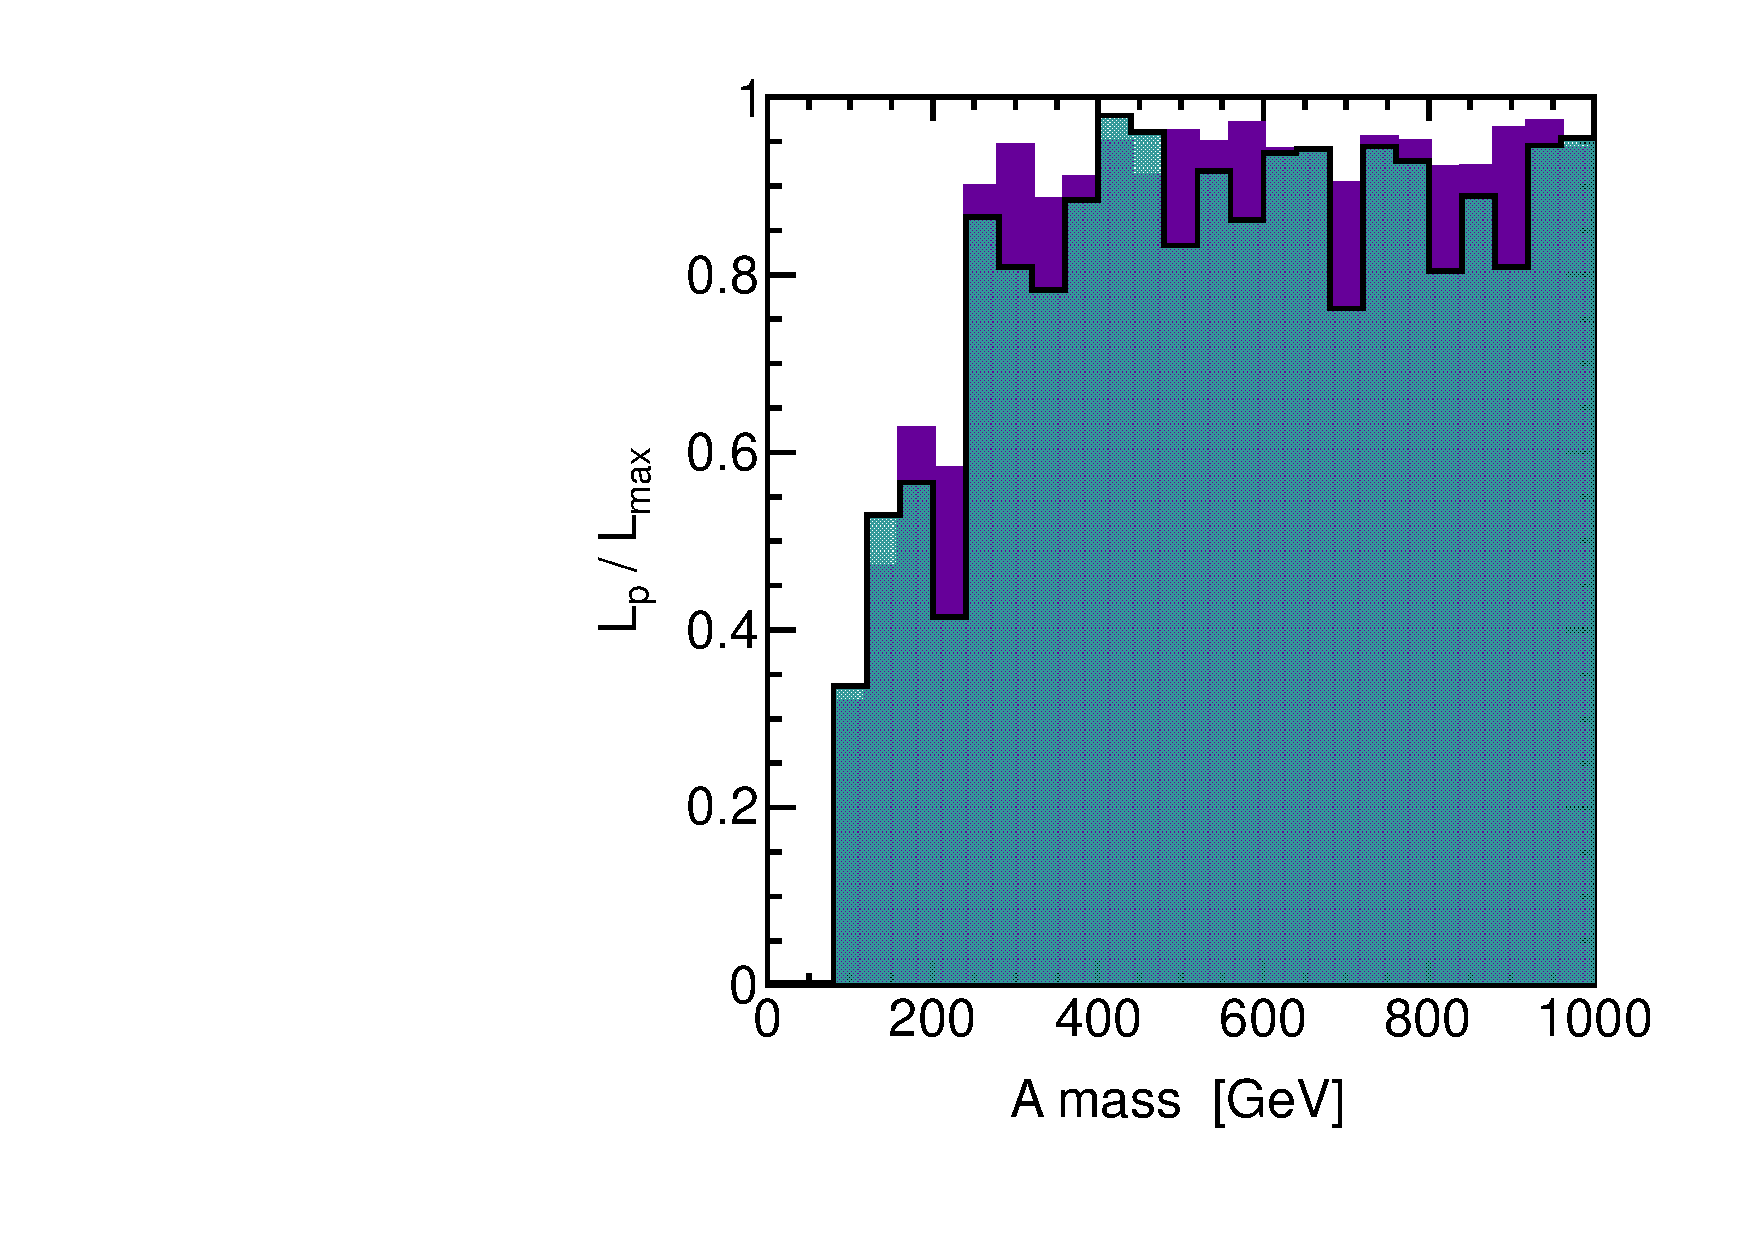
\includegraphics[height=5.5cm]{figs/fig_A.pdf} 
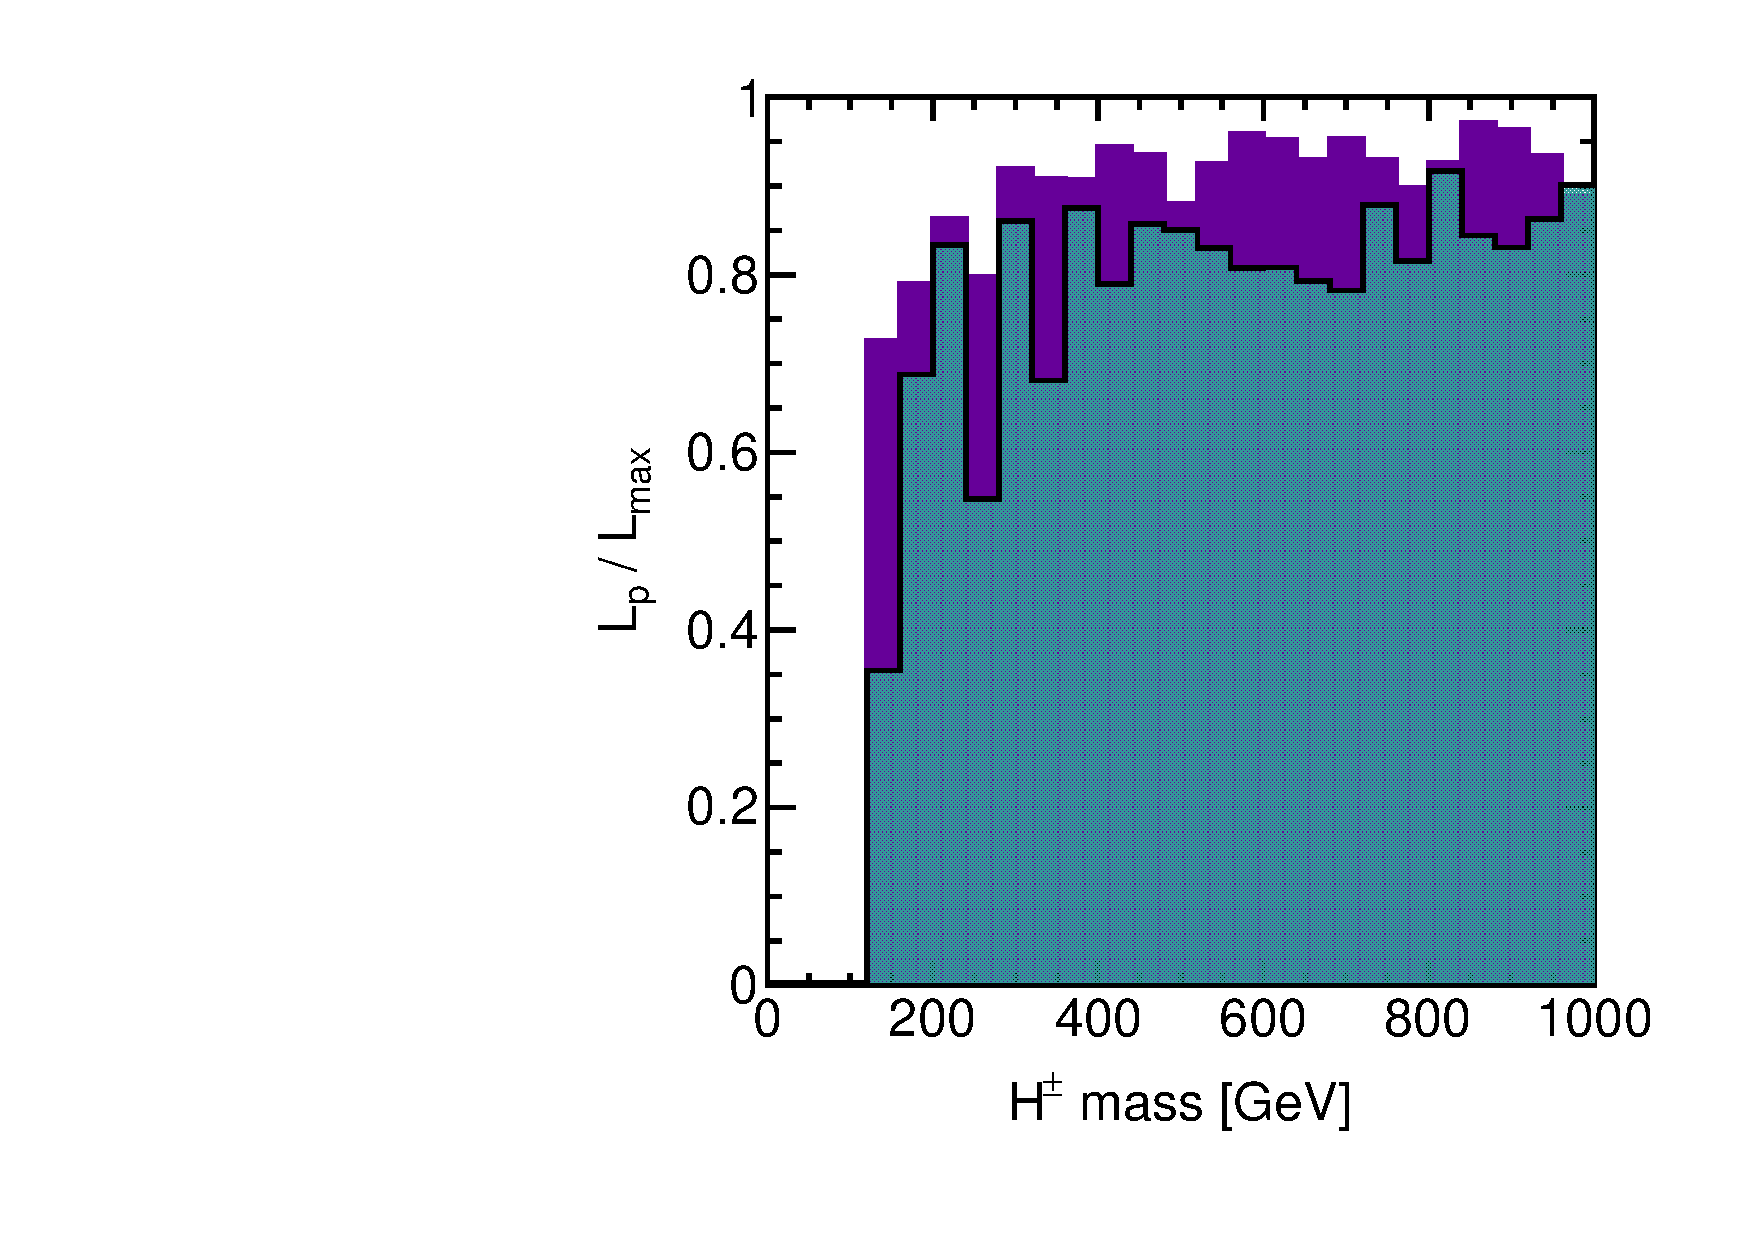
\includegraphics[height=5.5cm]{figs/fig_H_pm.pdf} 
\caption{Ratios of profile likelihood $L_p$ to maximum likelihood $L_{max}$ shown for the Higgs masses.  The colored and shaded histograms show the distributions before and after the inclusion of the CMS results.}
\label{fig:LRwcms_Higgs}
\end{center}
\end{figure}


\begin{figure}[htbp]
\begin{center}
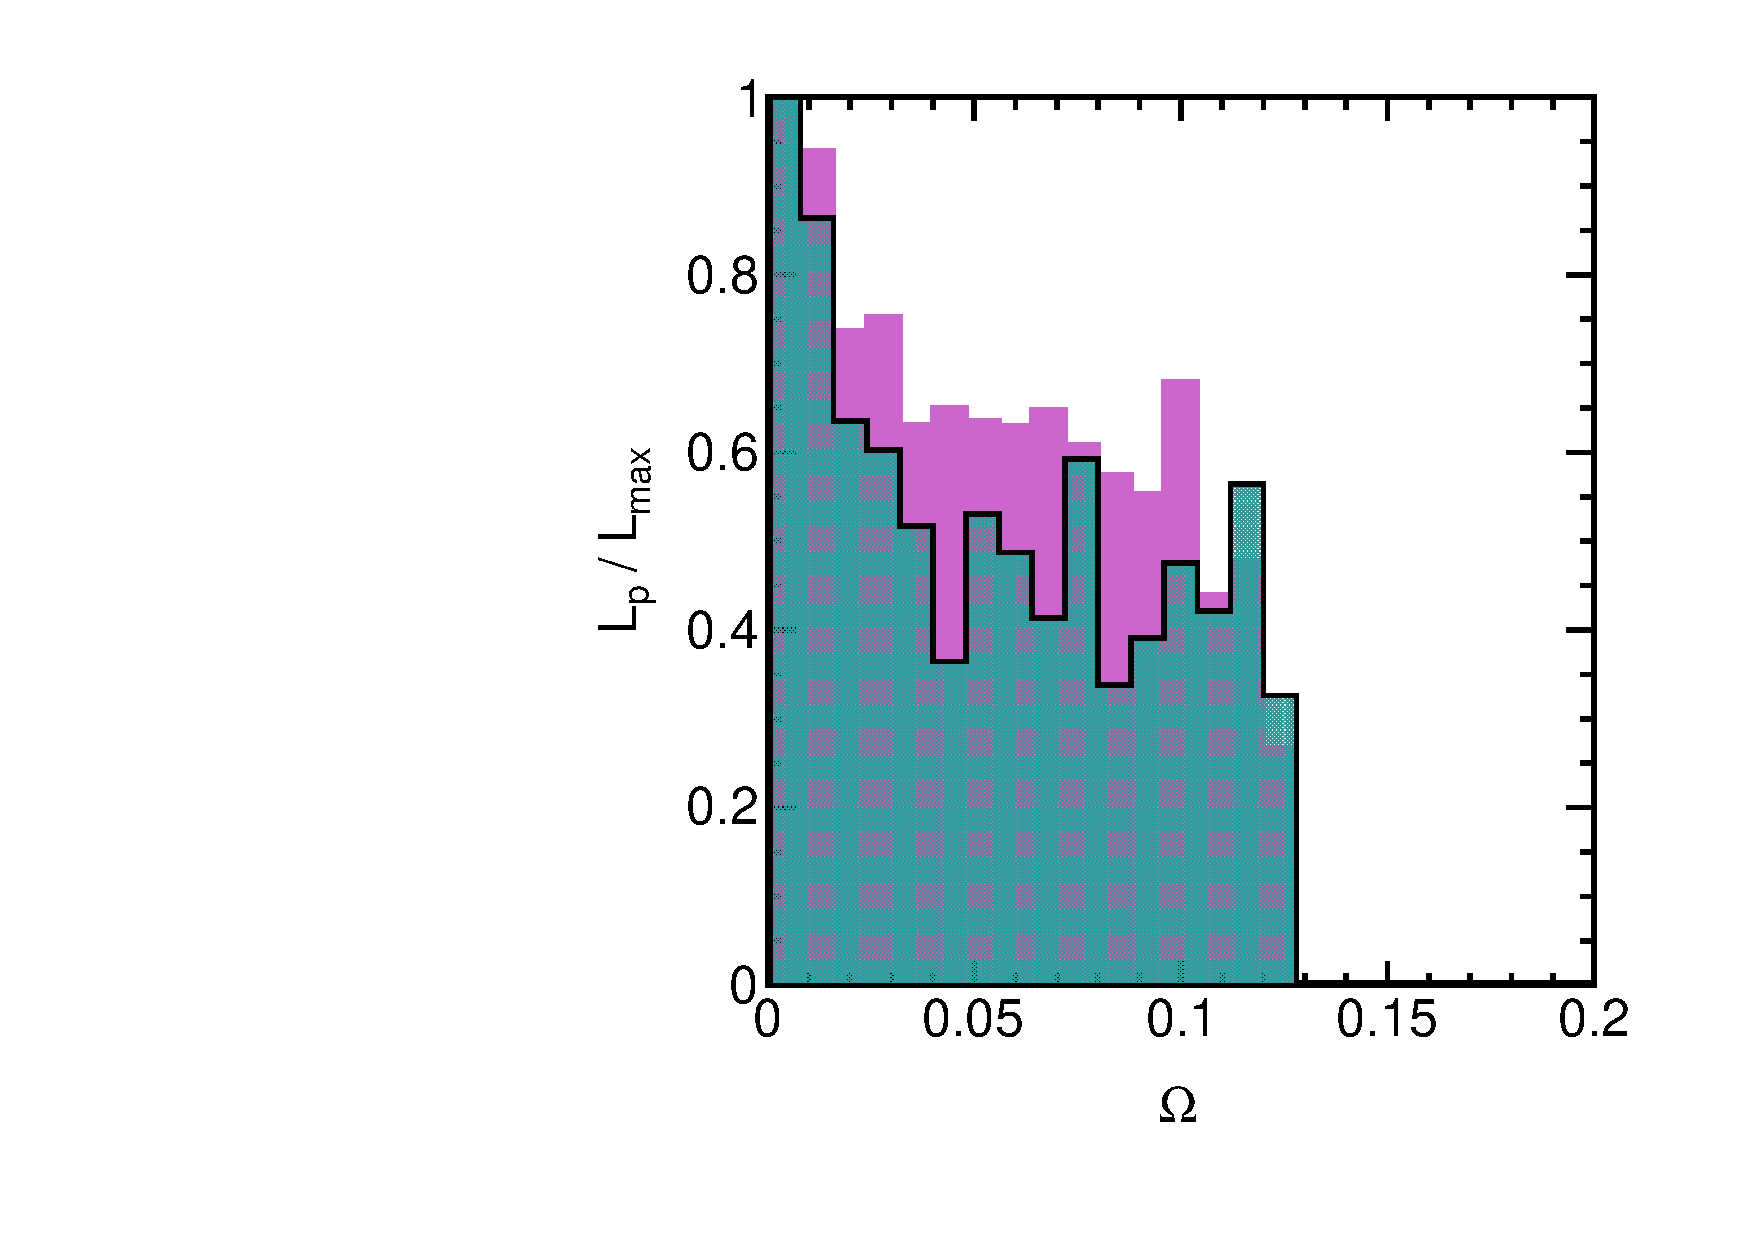
\includegraphics[height=5.5cm]{figs/fig_omega_m.pdf} 
\caption{Ratio of profile likelihood $L_p$ to maximum likelihood $L_{max}$ shown for lightest neutralino dark matter relic density.  The colored and shaded histograms show the distributions before and after the inclusion of the CMS results.}
\label{fig:LRwcms_omg}
\end{center}
\end{figure}


%\begin{figure}[htbp]
%\begin{center}
%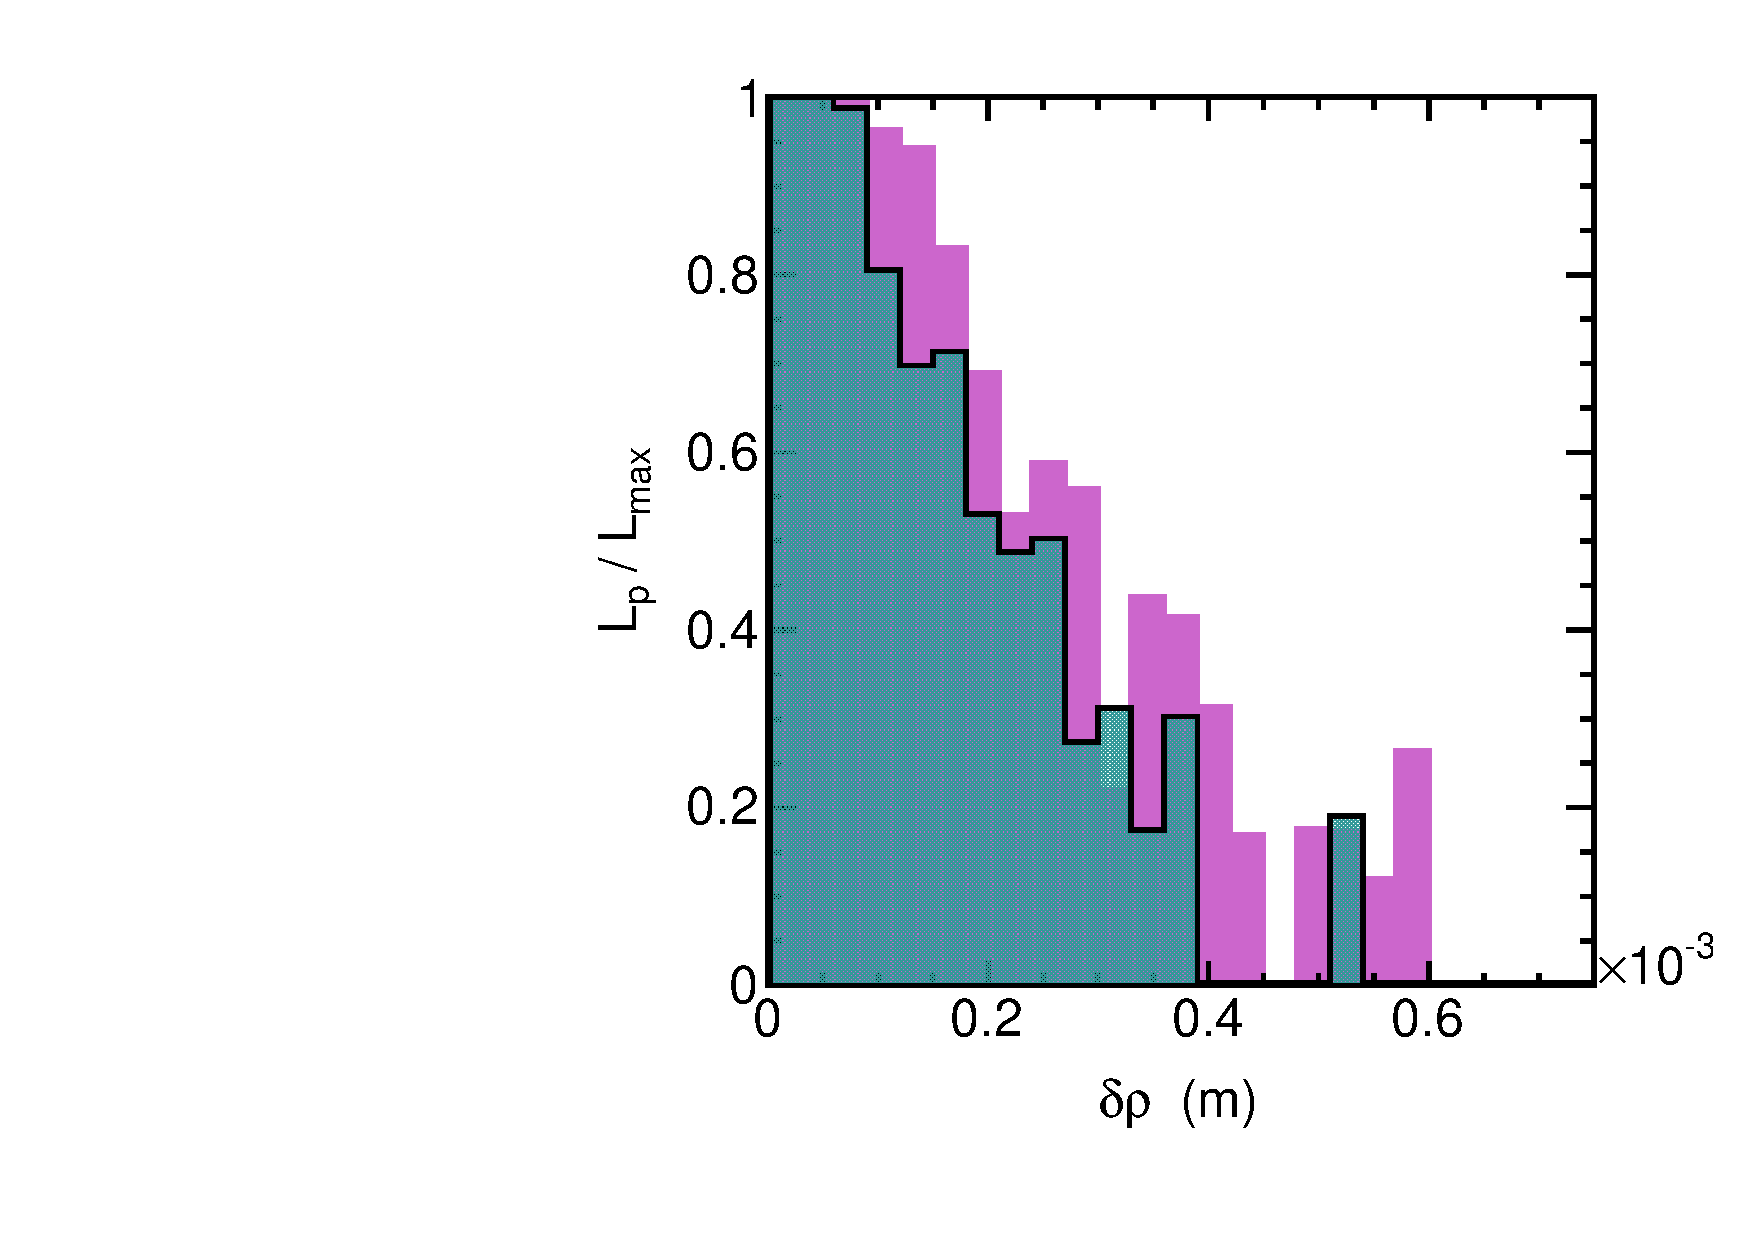
\includegraphics[height=5.5cm]{figs/fig_drho_m.pdf} 
%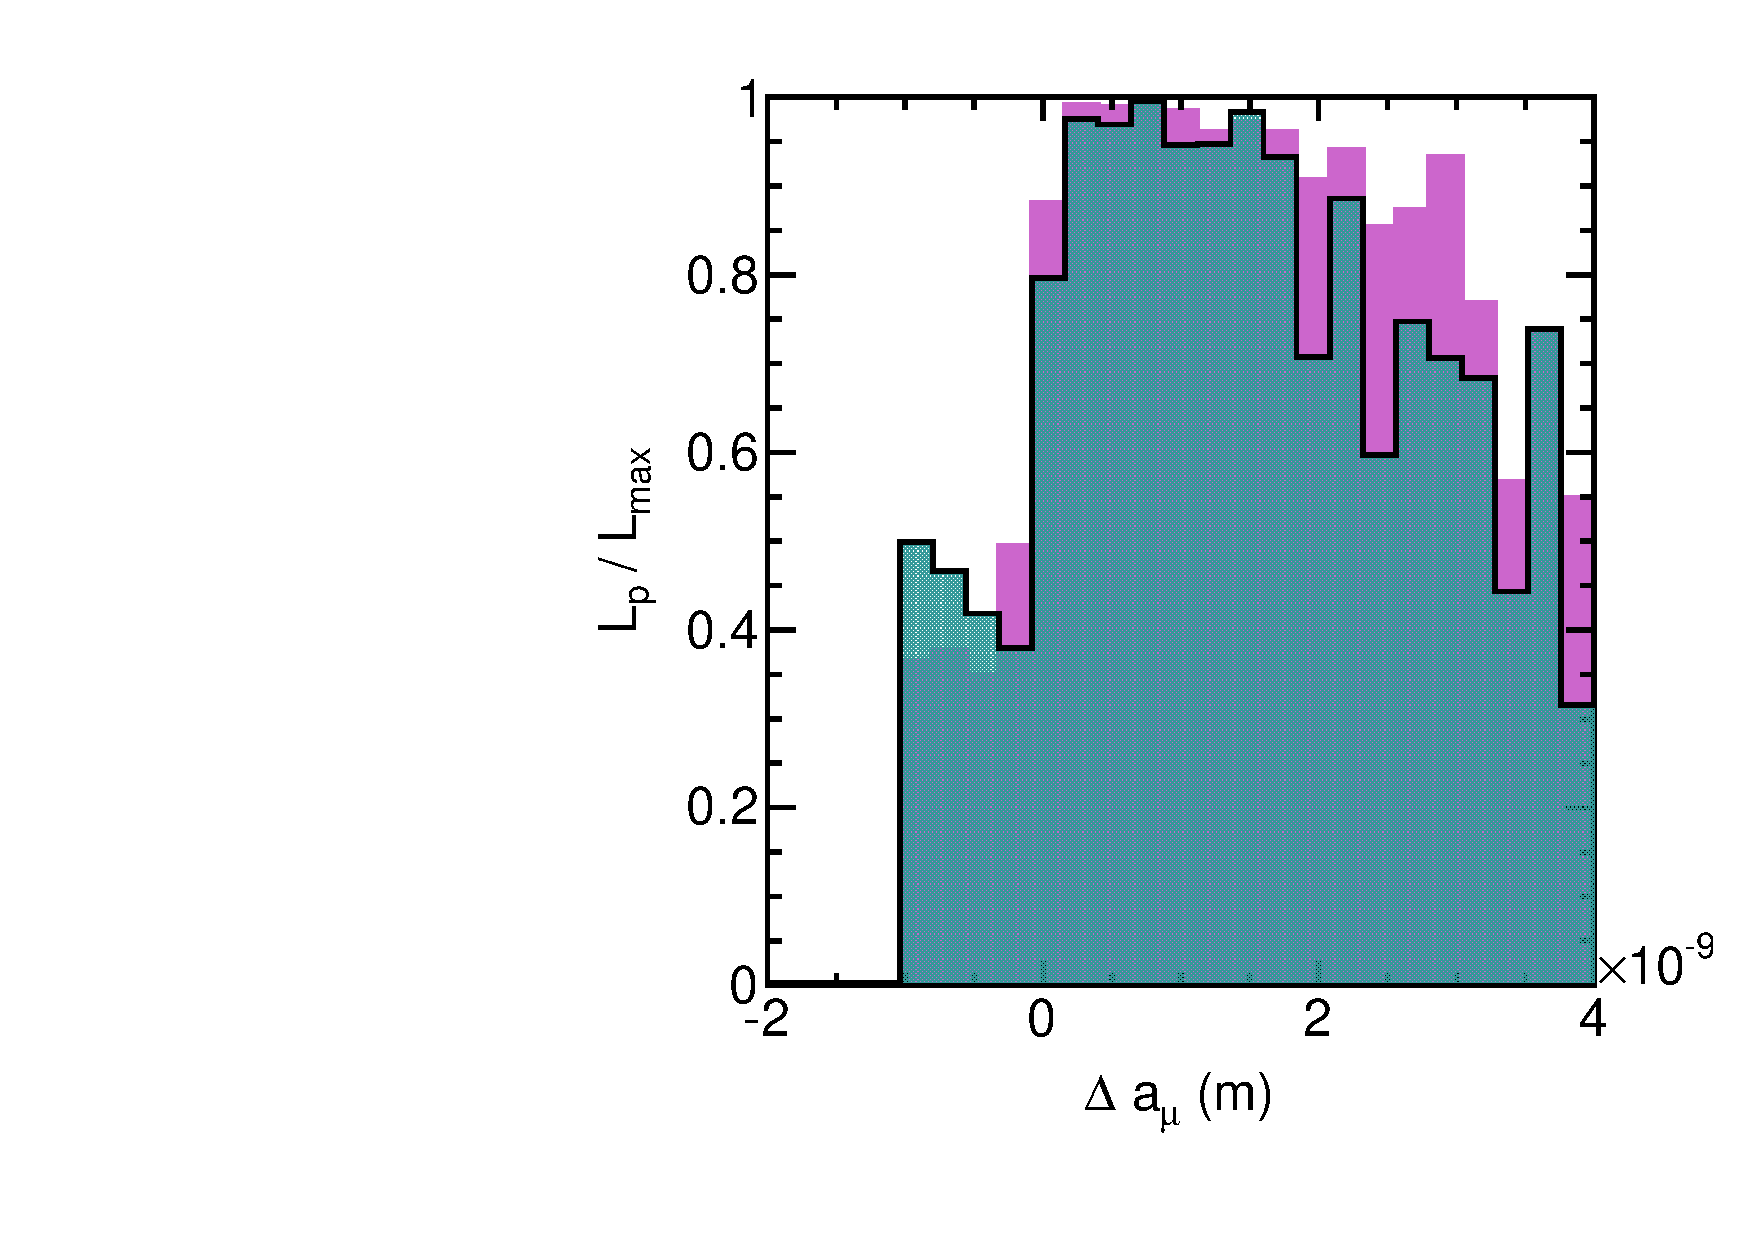
\includegraphics[height=5.5cm]{figs/fig_gmu_m.pdf} \\
%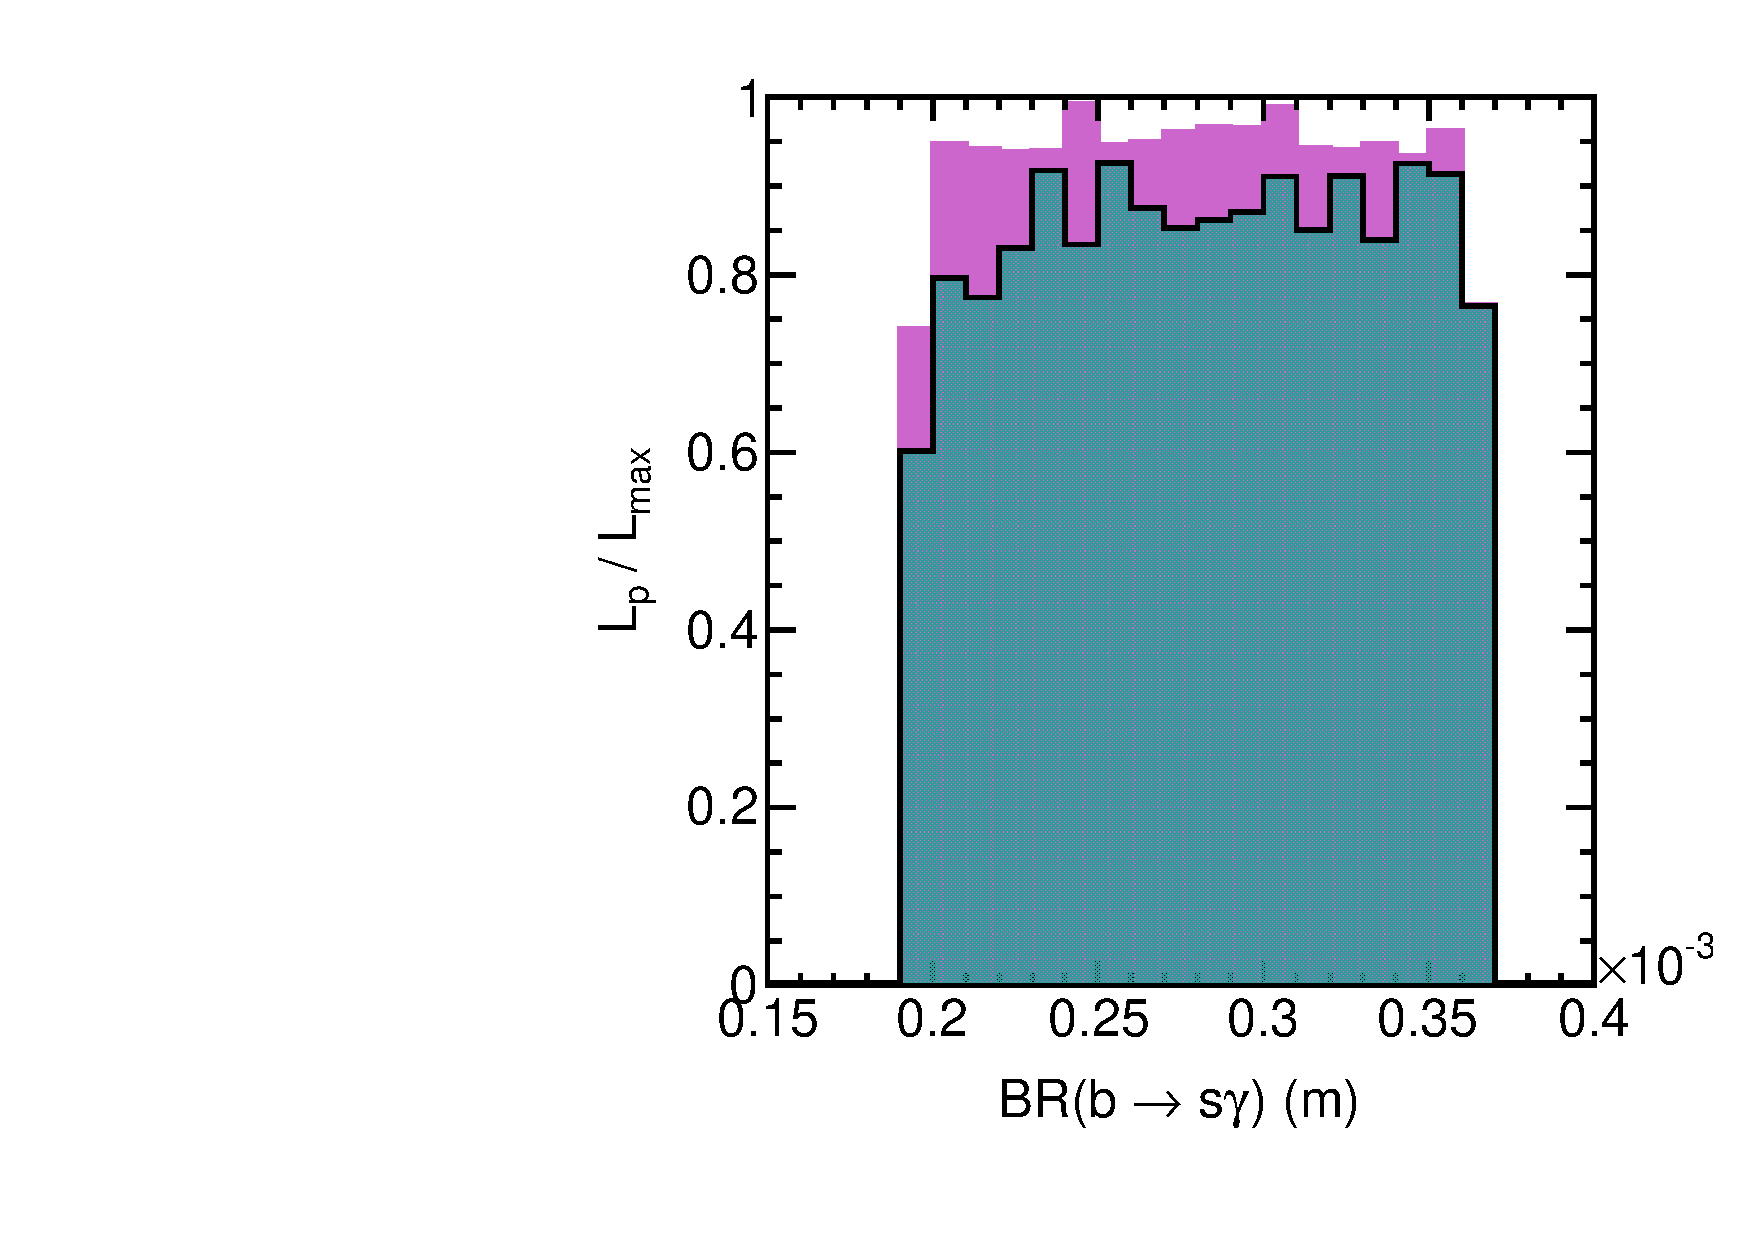
\includegraphics[height=5.5cm]{figs/fig_bsgamma_m.pdf} 
%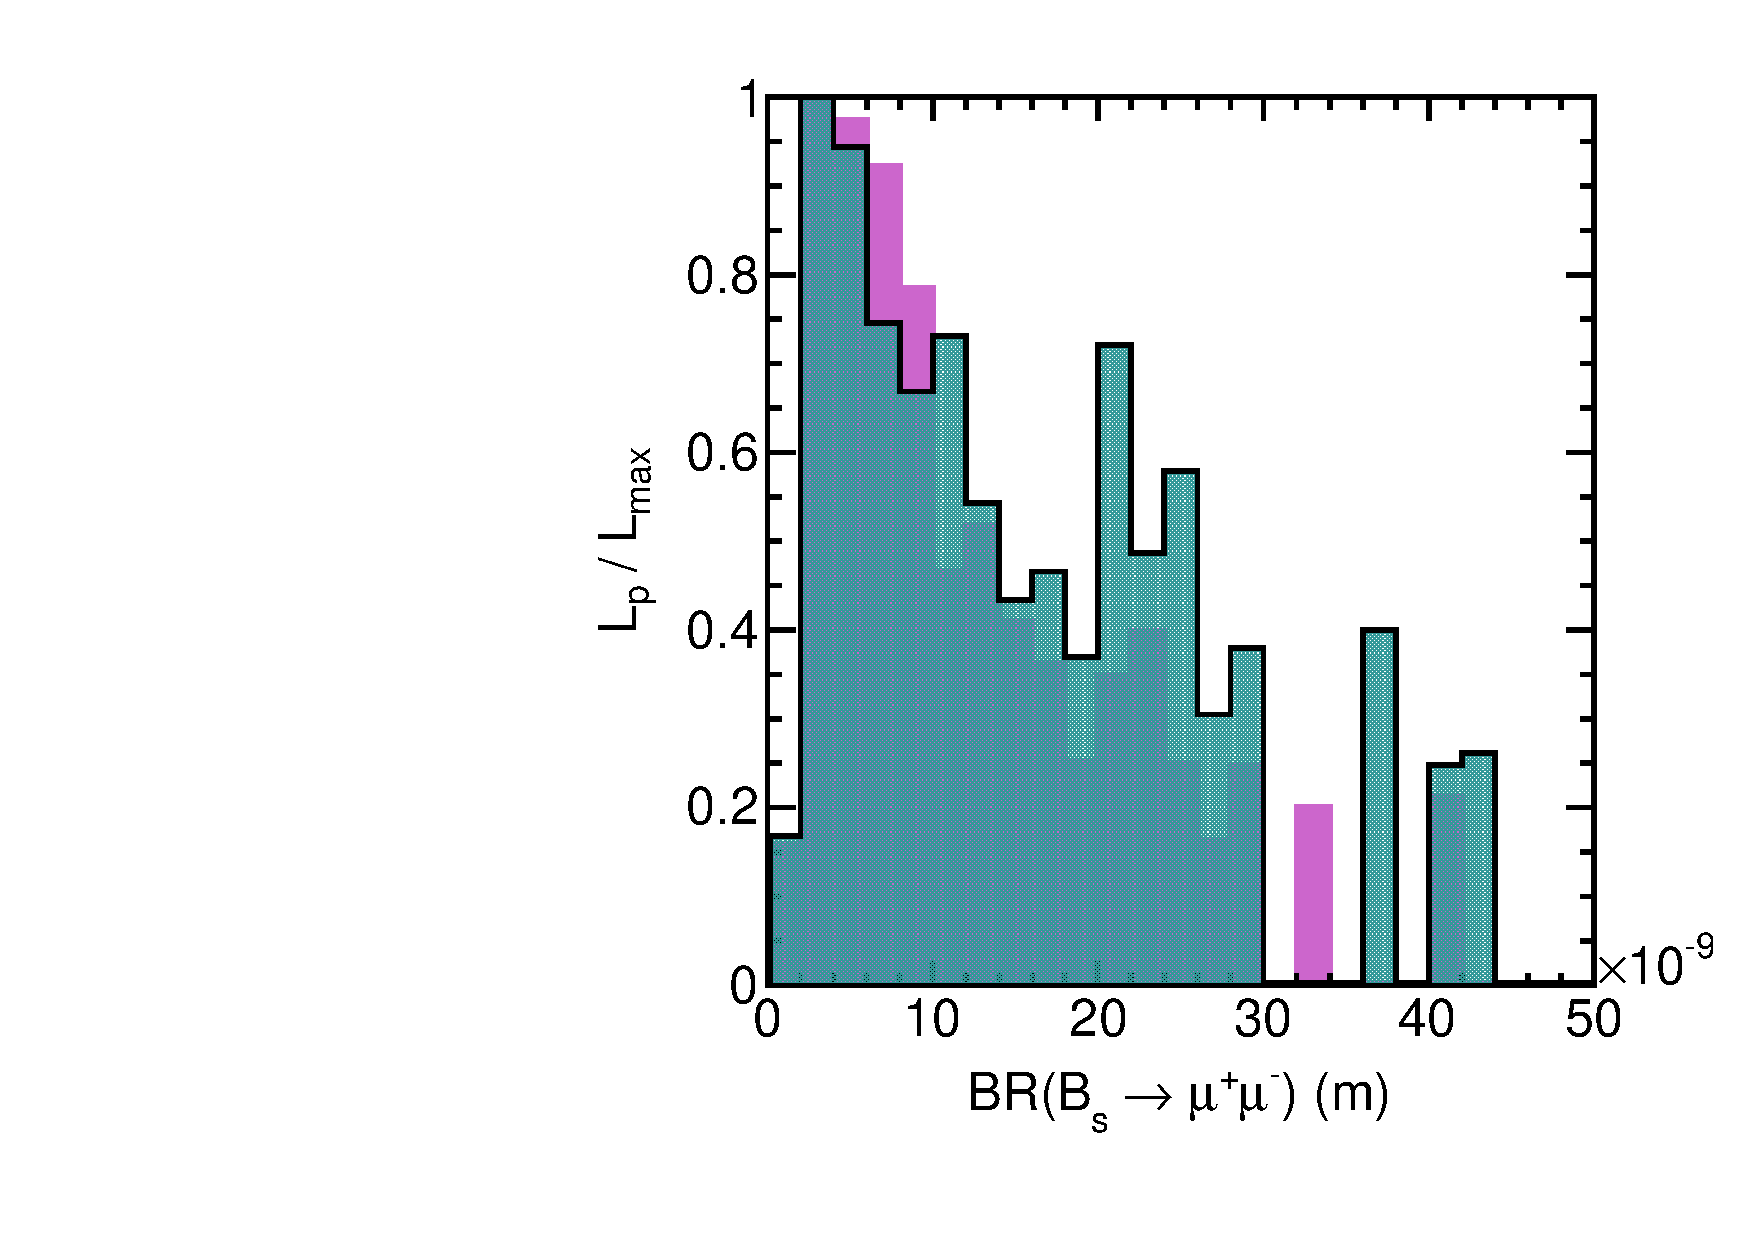
\includegraphics[height=5.5cm]{figs/fig_bsmumu_m.pdf} \\
%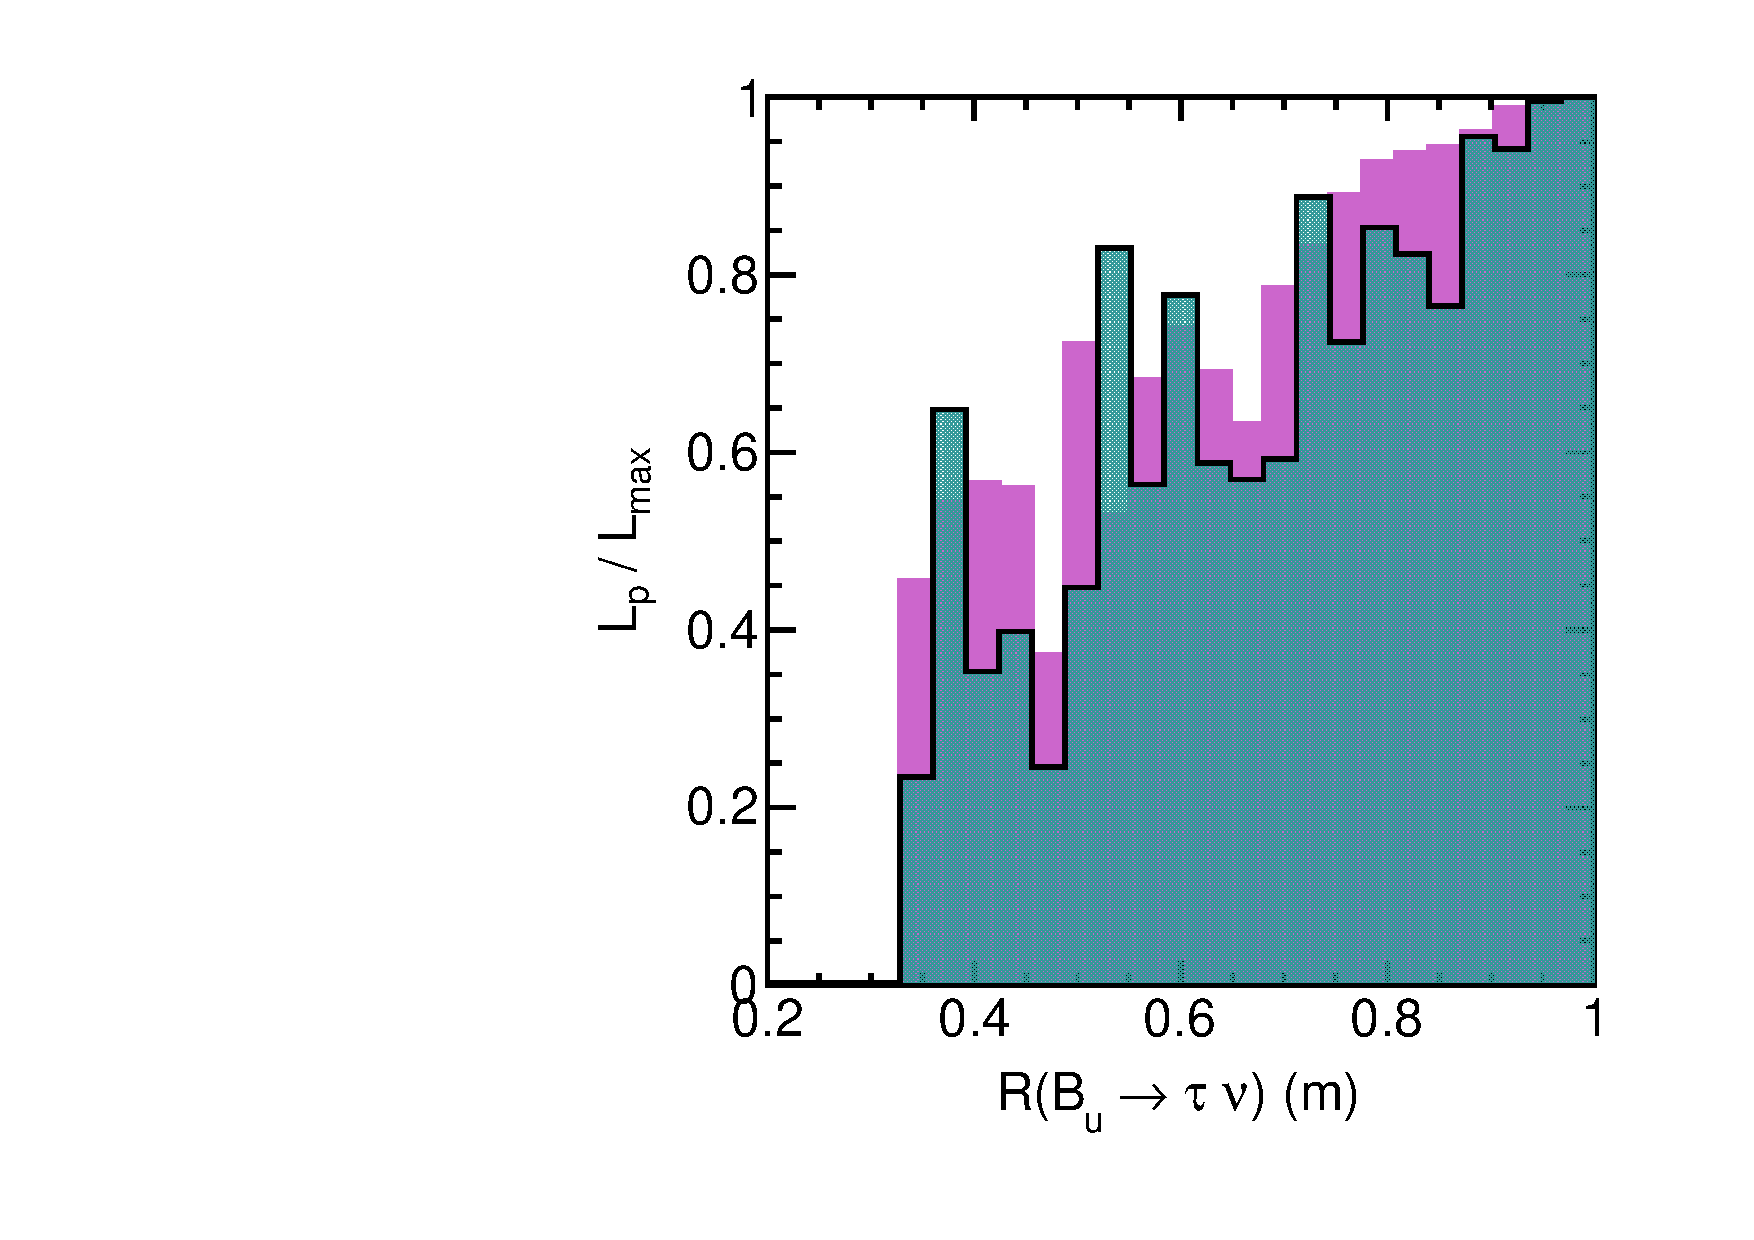
\includegraphics[height=5.5cm]{figs/fig_rbtaunu_m.pdf} 
%\caption{Ratios of profile likelihood $L_p$ to maximum likelihood $L_{max}$ shown for predictions for weak scale observables as calculated by micromegas.  The colored and shaded histograms show the distributions before and after the inclusion of the CMS results.}
%\label{fig:LRwcms_EWobs_m}
%\end{center}
%\end{figure}


\begin{figure}[htbp]
\begin{center}
%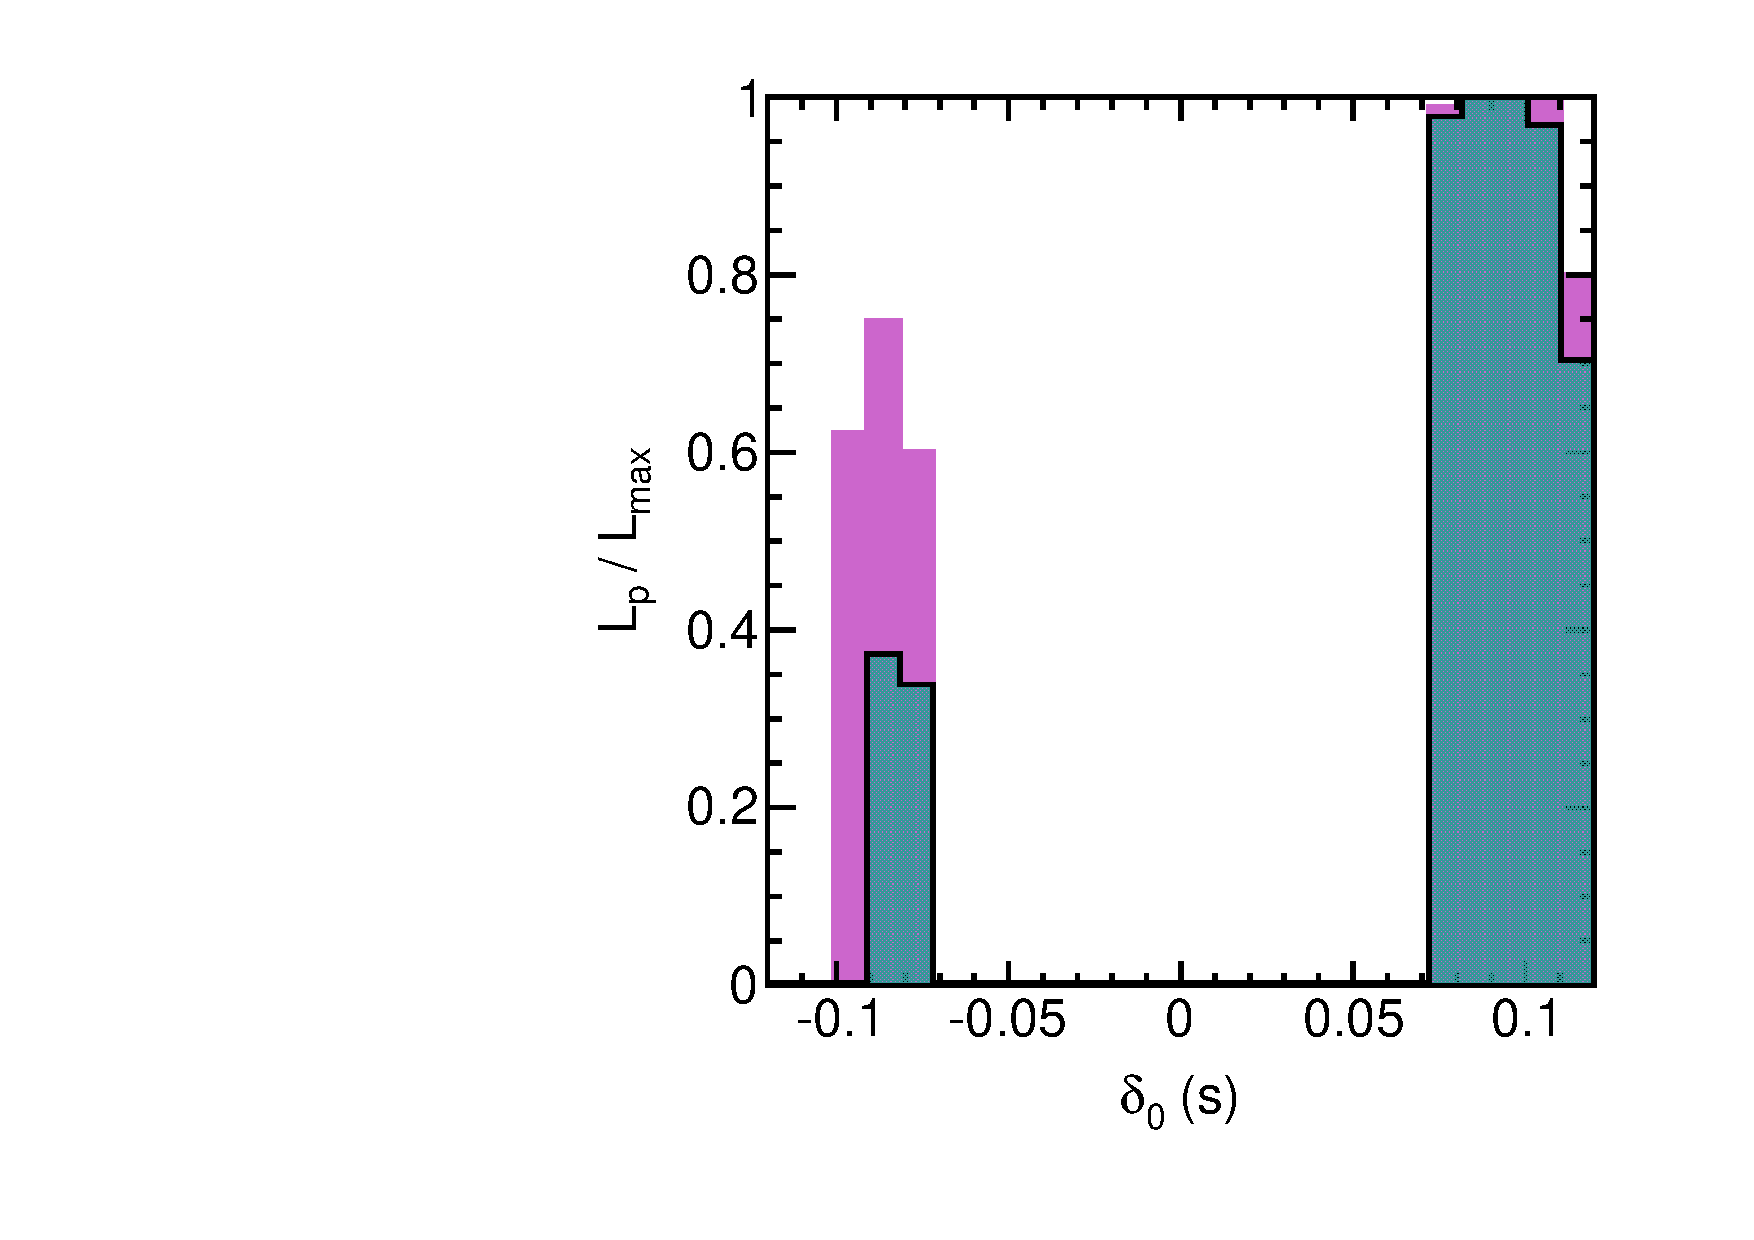
\includegraphics[height=5.5cm]{figs/fig_delta0_s.pdf} 
\includegraphics[height=5.5cm]{figs/fig_drho_m.pdf} 
\includegraphics[height=5.5cm]{figs/fig_muon_gm2_s.pdf} \\
\includegraphics[height=5.5cm]{figs/fig_bsgamma_s.pdf} 
\includegraphics[height=5.5cm]{figs/fig_Bsmumu_s.pdf} \\
\includegraphics[height=5.5cm]{figs/fig_Btaunu_s.pdf} 
\includegraphics[height=5.5cm]{figs/fig_RBtaunu_s.pdf} 
\caption{Ratios of profile likelihood $L_p$ to maximum likelihood $L_{max}$ shown for predictions for weak scale observables.  $\delta\rho$ is calculated using {\tt micrOMEGAs 2.4} and the rest are calculated using {\tt Superiso 2.7}.  The colored and shaded histograms show the distributions before and after the inclusion of the CMS results.}
\label{fig:LRwcms_EWobs_s1}
\end{center}
\end{figure}


\begin{figure}[htbp]
\begin{center}
\includegraphics[height=5.5cm]{figs/fig_BDtaunu_s.pdf} 
\includegraphics[height=5.5cm]{figs/fig_BDtaunu_BDenu_s.pdf} \\
\includegraphics[height=5.5cm]{figs/fig_Dmunu_s.pdf} 
\includegraphics[height=5.5cm]{figs/fig_Dsmunu_s.pdf} \\
\includegraphics[height=5.5cm]{figs/fig_Dstaunu_s.pdf} 
\includegraphics[height=5.5cm]{figs/fig_Kmunu_pimunu_s.pdf} \\
\includegraphics[height=5.5cm]{figs/fig_Rl23_s.pdf} 
\caption{Ratios of profile likelihood $L_p$ to maximum likelihood $L_{max}$ shown for predictions for weak scale observables as calculated by {\tt Superiso 2.7}.  The colored and shaded histograms show the distributions before and after the inclusion of the CMS results.}
\label{fig:LRwcms_EWobs_s2}
\end{center}
\end{figure}





